%  ========================================================================
%  Copyright (c) 1985 The University of Washington
%
%  Licensed under the Apache License, Version 2.0 (the "License");
%  you may not use this file except in compliance with the License.
%  You may obtain a copy of the License at
%
%      http://www.apache.org/licenses/LICENSE-2.0
%
%  Unless required by applicable law or agreed to in writing, software
%  distributed under the License is distributed on an "AS IS" BASIS,
%  WITHOUT WARRANTIES OR CONDITIONS OF ANY KIND, either express or implied.
%  See the License for the specific language governing permissions and
%  limitations under the License.
%  ========================================================================
%

% Documentation for University of Washington thesis LaTeX document class
% by Jim Fox
% fox@washington.edu
%
%    Revised for version 2015/03/03 of uwthesis.cls
%    Revised, 2016/11/22, for cleanup of sample copyright and title pages
%
%    This document is contained in a single file ONLY because
%    I wanted to be able to distribute it easily.  A real thesis ought
%    to be contained on many files (e.g., one for each chapter, at least).
%
%    To help you identify the files and sections in this large file
%    I use the string '==========' to identify new files.
%
%    To help you ignore the unusual things I do with this sample document
%    I try to use the notation
%       
%    % --- sample stuff only -----
%    special stuff for my document, but you don't need it in your thesis
%    % --- end-of-sample-stuff ---


%    Printed in twoside style now that that's allowed
%
 
\documentclass [11pt, proquest] {uwthesis}[2016/11/22]
 
%
% The following line would print the thesis in a postscript font 

% \def\bibpreamble{\protect\addcontentsline{toc}{chapter}{Bibliography}}

\setcounter{tocdepth}{1}  % Print the chapter and sections to the toc


% ==========   Local defs and mods
%

% --- sample stuff only -----
% These format the sample code in this document
\usepackage{hyperref} 
\usepackage{alltt}  % 
\usepackage{fontspec}
\usepackage{xspace}
\usepackage{microtype}
\usepackage{graphicx}
\usepackage{subfigure}
\usepackage{booktabs} % for professional tables
\usepackage{graphicx}
\usepackage{tikz}
\usepackage{amsmath}
\usepackage{amsfonts}
\usepackage[english]{babel}
\usepackage{blindtext}
\usepackage{bbm}
\usepackage{textcomp}
\usepackage{ulem}
\usepackage{tabularx}
\usepackage{enumitem}
\usepackage{xcolor}
\usepackage[font=small,skip=-0pt]{caption}
\usepackage{amsmath}

% \setmainfont[Ligatures=TeX]{DENG.TTF}
\newenvironment{demo}
  {\begin{alltt}\leftskip3em
     \def\\{\ttfamily\char`\\}%
     \def\{{\ttfamily\char`\{}%
     \def\}{\ttfamily\char`\}}}
  {\end{alltt}}
 
\definecolor{azureC}{RGB}{32,117,184}
\definecolor{ec2C}{RGB}{246,133,54}
 \newcommand{\pbox}{Parameter Box\xspace}
 \newcommand{\phub}{Parameter Hub\xspace}
 \newcommand{\plink}{Parameter Link\xspace}
 \newcommand{\pseries}{Parameter\xspace}
 \newcommand{\azure}{\textcolor{azureC}{Azure}\xspace}
\newcommand{\ectwo}{\textcolor{ec2C}{EC2}\xspace}
%\newcommand{\marcopolo}{Marcopolo\xspace}
\newcommand{\marcopolo}{ProbeEmbed\xspace}
\newcommand{\ha}{AggEngine\xspace}
\newcommand{\mlha}{2LHA\xspace}
\newcommand{\strongrandom}{Balanced Random\xspace}
\newcommand{\autoplink}{Autotune\xspace}
\newcommand{\code}[1]{\texttt{\small{#1}}}
\newcommand{\strongbaseline}{strong baseline\xspace}
\newcommand{\psliteib}{\mxnet IB\xspace}
\newcommand{\pshard}{PShard\xspace}
\newcommand{\pswitch}{PSwitch\xspace}

\newcommand{\cmpilogo}{%
  \begingroup\normalfont
  
\includegraphics[height=\fontcharht\font`\B]{Figures/cloud.png}%
  \endgroup
}

\newcommand{\mpiC}{Collectives\xspace}
\newcommand{\mpi}{collectives\xspace}
\newcommand{\collectives}{\mpi}
\newcommand{\cmpi}{\cmpilogo\xspace{}\mpiC}


% metafont font.  If logo not available, use the second form
%
% \font\mffont=logosl10 scaled\magstep1
\let\mffont=\sf
% --- end-of-sample-stuff ---
 



\begin{document}
 
% ==========   Preliminary pages
%
% ( revised 2012 for electronic submission )
%

\prelimpages
 
%
% ----- copyright and title pages
%
\Title{Towards More Efficient Communication for Distributed Learning Systems}
\Author{Liang Luo}
\Year{2020}
\Program{Computer Science and Engineering}

\Chair{Luis Ceze}{Professor}{Computer Science and Engineering}
\Signature{Arvind Krishnamurthy}
\Signature{Zachary Tatlock}
\Signature{Eric Klavins}
\Signature{Jacob Nelson}


\copyrightpage

\titlepage  

 
%
% ----- signature and quoteslip are gone
%

%
% ----- abstract
%


\setcounter{page}{-1}
\abstract{%
The explosion of data volume and ever-increasing speed of accelerators shift the bottleneck of large-scale distributed training tasks from computation to communication. We observe significant pressure on the communication backends of various mainstream learning systems in multiple environments when running such tasks. Achieving efficient large scale learning relies on more effective communication plane. 

We provide detailed analysis that root-causes the reasons affecting the communication efficiency of these systems in the context of different environments. We pinpoint bottlenecks from the software, hardware and network infrastructure stacks. 
  

We show how these obstacles can be overcome with a systematic codesign of a streamlined communication stack, a balanced hardware and cluster configuration with the distributed training workload, together with awareness of network topology and environment. We show this series of approaches, named \pbox, \phub , \plink along with \cmpi, accelerate distributed training from small clusters to datacenters and all the way to the commercial clouds while providing varying degrees of customization to suit different needs.}
%while allows for variable degree of transparency: the \pseries series enables solutions with no code change required to full customization of hardware.
%}
 
%
% ----- contents & etc.
%

%\listoftables  % I have no tables
 
%
% ----- glossary 
%
%\acknowledgments{% \vskip2pc
  % {\narrower\noindent
%  The author wishes to express sincere appreciation to
%  University of Washington, where he has had the opportunity
%  to work with the \TeX\ formatting system,
%  and to the author of \TeX, Donald Knuth, {\it il miglior fabbro}.
  % \par}
%}

%
% ----- dedication
%
\dedication{\begin{center}Thank you to my parents, Changyi and Yanan, for your endless love and support.

Thank you to my academic advisers, Luis Ceze and Arvind Krishnamurthy, for patiently guiding me through the process.

Thank you to this committee for keeping me on track. 



Thank you to my friends for the joy and laughter in the journey.

\end{center}}
\textpages

\section{Introduction}
Today, learning systems have gained significant attention in the literature for the overwhelming popularity of machine-learning (ML) related workloads. Most of work to date in the systems and architecture community has focused on improving the efficiency of evaluating trained models. This makes sense given that a model is trained only once but can be used many times for inference. However, arriving at a trained model frequently requires experimentation, and thus multiple training runs, each of which may take days. Accelerating the training process lets ML scientists iterate faster and design better model.

Traditionally, training has been viewed as a compute-bound problem, best done in a single large compute node with many accelerators. However, the ever-growing data volume pushes for monster-sized models, a scale even the exponentiation of compute power growth in single device couldn't handle. As ML models get bigger, training time gets prohibitively longer. Timely training requires exploiting parallelism with a distributed system.

\begin{table}
\centering
\begin{tabular}{|c|c|c|c|c|}
  \hline
  Models & Complexity & Size & Time & Configuration \\
  \hline
  Linear Regression~\cite{seber2012linear} & O($D^3+ N^2D$) & Small & Short & CPU \\
  \hline
  SVM~\cite{wang2005support} & O($N^2D^2$) & Small & Short & CPU \\
  \hline
  GBDT~\cite{friedman2001greedy} & O($TLFN$) & Small & Short & A few CPUs \\
  \hline
  \hline 
  AlexNet~\cite{alexnet}   & 0.0058 & 48M & 6 days  & 2x GTX 580\\
  \hline
  ZFNet~\cite{ZFNet}   & 0.0062  &  $\approx$48M  & 12 days  & GTX 580\\
  \hline
  VGGNet~\cite{VGGNet}   & 0.12  & 137M & 15 days & 4x Titan Black\\
  \hline
  GoogleNet~\cite{GoogleNet}   & 0.03  & 9M & 7 days & A few GPUs\\
  \hline
  ResNet~\cite{RESNET}   & 0.117 &  58M & 21 days & 8x GPUs\\
  \hline
  Xception~\cite{Chollet_2017}  & 5.0  & 22M & 30 days & 60x K80\\
  \hline
  \hline
  BERT~\cite{bert}  & 3.8 & 340M & 4 days & 16x TPUs v2 \\
  \hline
  GPT-2~\cite{GPT2}  & 248 & 1.5B & 7+ days~\cite{gpt2Time} & 256x TPUs v3 \\
  \hline
  \hline
%  Device Placement~\cite{mirhoseini2017device} 2017 & - & 27 hours & 80 GPU nodes  \\
%  \hline
  NAS~\cite{zoph2016neural}  & 31 & 86M & 28 days & 800 K40 GPUs\\
  \hline
  AlphaGoZero~\cite{silver2016mastering}  & 1800 & - & 1 day & 5000x TPUs \\
  \hline
\end{tabular}
\caption{A few representative machine learning techniques and models that support increasingly complex tasks (trees, support vector machines, neural networks) and their complexities to train (pfs-day, or days to train computing at 1 PFlop/s. 1PF/s roughly corresponds to 64 Tesla V100 GPUs FP32, or 8 with mixed-precision FP16, running at peak throughput), and their reported training time and the machines they are trained on. We used the same method of estimating complexity as in the original OpenAI blog post~\cite{AIandCom3:online} for the additional models in the table. $D$: features. $N$: samples. $L$: leaves per tree. $T$: number of trees to build.}
\label{table:trend}
\end{table}

Table~\ref{table:trend} gives a taste of the evolution of machines learning models/techniques: they are getting increasingly more demanding in terms of compute resources, such that the use of hundreds or even thousands of machines and accelerators for weeks is commonplace. 




The most common way of exploiting parallelism, ``data'' parallelism, consists of a computation-heavy local computation phase and a communication-heavy parameter exchange phase. Efficient distributed training involves optimizing both stages. Many past work demonstrate the solution of accelerating these processes by building specialized hardware clusters with fast interconnects ~\cite{DBLP:journals/corr/abs-1711-00489, You:2018:ITM:3225058.3225069, DBLP:journals/corr/abs-1711-04325,jia2018highly,DBLP:journals/corr/abs-1811-05233,sun2019optimizing, ImageNetIn1Hour, firecaffe, phubsocc}. While the results are encouraging, as we shall see, faster hardware is not panacea: the unstreamlined software stack and unbalanced compute to communication resource allocation prohibits utilizing full capability of the hardware, and the compute units are more likely than not waiting on the network because the latter simply cannot keep up (Figure~\ref{fig:clusterOverhead}). We expect the problem not going away on its own, because of the observed trend at which the network capability is growing is significantly outpaced by that of the compute resources (Figure~\ref{fig:accthroughput}).  


\begin{figure}
	\centering
	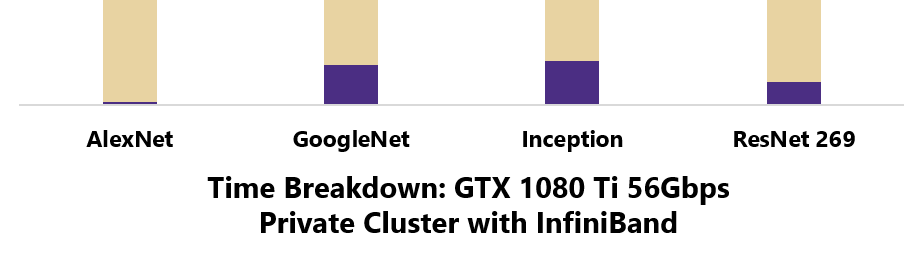
\includegraphics[width=.5\linewidth, trim=6 1 3 3,clip]{Figures/clusteroverhead.png}
	\caption{Even with a fast, small-scale cluster, communication still takes most of the time duration training, wasting compute resources.}
	\label{fig:clusterOverhead}
\end{figure}

\begin{figure}
	\centering
	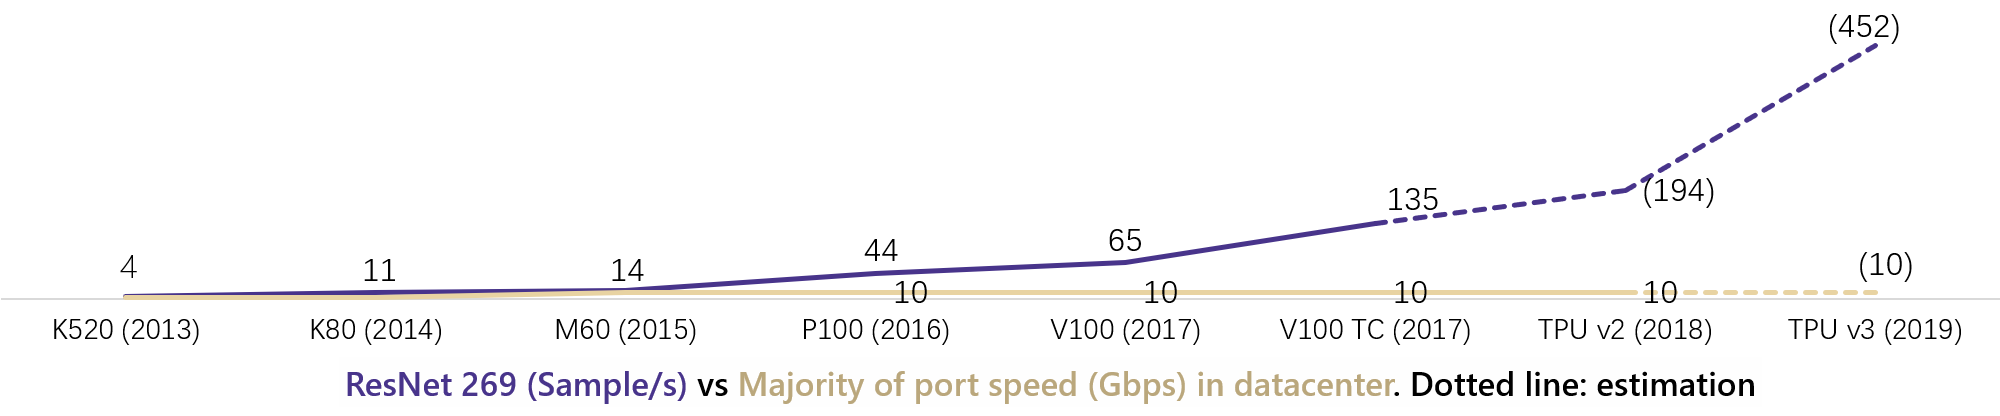
\includegraphics[width=\linewidth, trim=2 3 3 3,clip]{Figures/computevscomm.png}
	\caption{Throughput for an industry standard benchmark (ResNet) has seen an improvement of 35x, and is estimated to increase by 100x with latest accelerators. GPU performance tested with MxNet on EC2. TPU throughput estimated based on TensorCore's measured performance. Estimation for majority of the port speed of datacenters is based on Cisco study~\cite{CISCOMarket}. Only until very recently did the public cloud start offering 100Gbps bandwidth instances on standalone VMs~\cite{Introduc9:online, NewC5nIn6:online}}.
	\label{fig:accthroughput}
\end{figure}

To tackle these problems, a comprehensive codesign of software stack and hardware configuration is required. To that end, we provide a template for speccing an entity called \pbox that provides the near perfect communication to computation balance for acting as a parameter server in a distributed training job, and a companion piece of software, \phub that streamlines handling over gradient  transfer, aggregation and model optimization by carefully extracting locality inside a physical host and latency hiding. 

While \pbox and \phub are effective, it is important to understand accelerating training in these specialized, privately-owned clusters does not complete the story: first, those hardware setups require steep investment and only a few have that luxury; second, since it is much easier to thoroughly optimize the entire stack in private clusters as we have control over the entire system, some optimizations are not always possible to be applied universally.

An alternative to owning a private cluster is renting VMs from the public cloud, which has become a popular, more accessible approach. Currently, all major cloud providers offer racks of nodes with specialized accelerators (such as GPUs, TPUs, and custom FPGAs)~\cite{GoogleCl74:online,MachineL50:online,DeepLear23:online,sagemaker,brainwave,Jouppi:2017:IPA:3079856.3080246,222611} for ML workloads. But at the same time, scalable training in the public cloud isn't just a straightforward application of \pbox and \phub optimizations.

\begin{figure*}[t!]
	\centering
	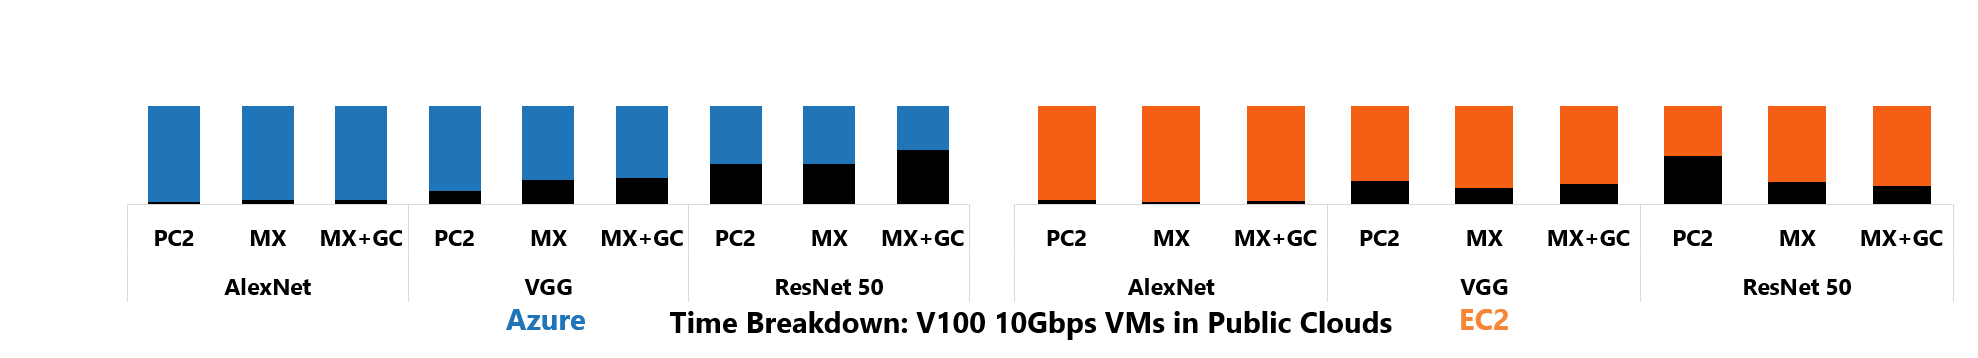
\includegraphics[width=.9\linewidth, trim=6 1 3 3,clip]{Figures/cloudoverhead.png}
	\caption{Even with state of the art training frameworks and recent optimizations, up to 90\% of time during cloud-based training of popular models is wasted explicitly waiting on the network in the public clouds.}
	\label{fig:cloudOverhead}
\end{figure*}


Even with modern frameworks and recent optimizations 
(e.g., gradient compression and quantization~\cite{lin2017deep, cntk1bt, lim20183lc}, latency-hiding~\cite{poseidon, jayarajan2019priority,hashemi2018tictac}, optimized communication libraries~\cite{facebook35:online, Operatio73:online, dmlcpsli50:online} and large batch optimizations~\cite{ImageNetIn1Hour}), distributed training at scale on the public cloud still incurs high overhead: up to 90\% of total training time can be wasted waiting on the network (Figure~\ref{fig:cloudOverhead}). Further, existing solutions so far focus solely on addressing the \textit{bandwidth} bottleneck, and ignores cloud-specific challenges: the hierarchical network structure in datacenter breaks the usual assumption of link speed being uniform; multi-tenancy and the dynamic nature of the cloud traffic cause high variation in performance. All these add to the complexity of scaling up distributed training and can render existing solutions less effective. 

Accelerating cloud-based distributed training thus requires paying attention to a third dimension (apart from software and hardware): the environment. First, we need an aggregation mechanism that is appropriate for network topologies that display bandwidth oversubscription, and that makes appropriate use of underprovisioned links.  Second, we need to be able to identify the underlying network topologies and bandwidth/latency constraints (or collectively, locality) even if the public cloud does not expose such information.  Finally, we need communication schemes that can react to changing network conditions, especially in the presence of interfering traffic generated by other tenants. Our solution is collectively called \plink, an optimized, locality-aware system that uses a fitted hierarchical aggregation scheme to extract locality from the underlying datacenter network, based on end-to-end network probes and dynamic network load.

With \pbox, \phub and \plink, we complete the picture of accelerating machine learning of all kinds, ubiquitously. In the following sections, we start with an overview of the mechanism of distributed training, then we walk through each of the proposed solution in detail. We show how specific optimizations adopted target directly at the bottlenecks in each scenario and lead to end-to-end speedup in real-world learning tasks.
\section{Background}
We now establish conventions used in this paper, and familiarize the reader with basic concepts for distributed training.


\subsection{Training a ML model}
Different types of models may appear to have different ways of training, but sitting at the center of most models is the common notion of parameters and gradients. Parameters are the goals: they define the ultimate models; gradients are the means: they are derived with respect to parameters, and guide how parameters should be adjusted to minimize the errors together with a learning rate, usually in an iterative manner, using the technique (or its variant) gradient descent~\cite{subgradient,DBLP:journals/corr/Ruder16}. 

To illustrate the training process, we use the example of training a deep learning (DL) model, or a deep neural network (DNN), for its popularity. We will continue to explain in the context of DL models throughout this paper for consistency. Modern DL models can have hundreds of \textit{layers} making up multi-megabyte-size \textit{models}. The training process has three phases. In the \textit{forward pass}, a prediction is generated for an input. In the \textit{backward pass}, the prediction is compared with a label to calculate prediction error; then, through \textit{backpropagation}~\cite{backprop}, the gradient for each parameter
is calculated with respect to this error. The model is then \textit{updated} using these gradients, often using a variant of the gradient descent optimization algorithm. Each Computation is often done on GPUs or other accelerators suited to regular data-parallel operations, processing a batch of samples at once (\textit{minibatching}).
%Multiple examples are processed in each GPU simultaneously in a single \emph{minibatch} which typically contains tens to hundreds of samples. 
%Each GPU processes multiple examples simultaneously in a \emph{minibatch} which typically contains tens to hundreds of samples. 

\begin{figure}[t!]
	\centering
	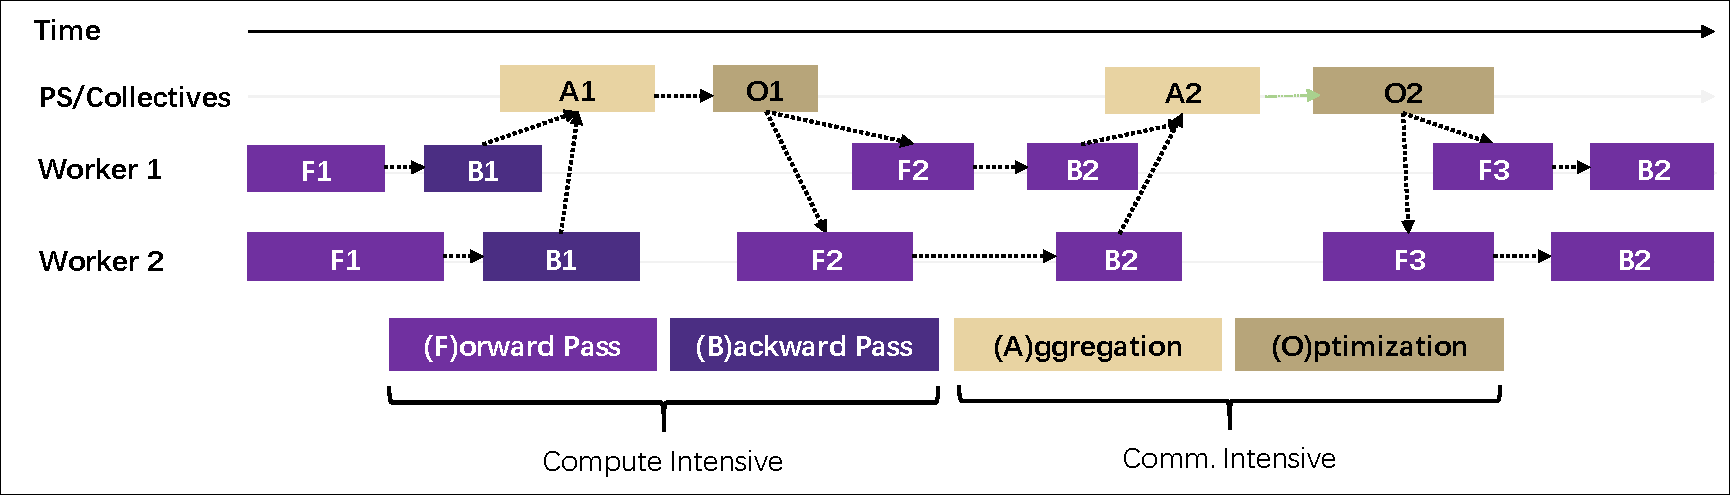
\includegraphics[width=\linewidth, trim=2 3 3 3,clip]{Figures/distributedtraining.pdf}
	\caption{A few iterations of distributed training pipeline of neural networks.}
	\label{fig:distributedtraining}
\end{figure}

\subsection{Distributed Training}
Broadly speaking, there are two extremes in terms of paradigms in distributed training: \textit{data} parallelism and \textit{model} parallelism, and many hybrid systems strike a balance between this two.

In data parallelism, there is the notion of \textit{workers} and \textit{servers}, two non-exclusive roles a node can take. Training data is prepartitioned to each individual workers, and servers store the current model parameters in a sharded manner. In the computation phase of each iteration, no data is exchanged until all workers derive the gradients; gradients are then sent to servers for processing.

In model parallelism, instead of partitioning training data, the model itself is being partitioned. This is handy because the multi-layer of modern DL models and well-defined dependencies make it simple to partition the model to different nodes. A piece of data then follows through the entire system, as if in the single node training case, except that it crosses node boundaries.

This paper mainly focuses on data parallelism, as it is the default choice in many frameworks and practices. The distributed training process (Figure~\ref{fig:distributedtraining}) using data parallelism is different in a few ways from training within a single node.
%First, a mean gradient is calculated for each minibatch in each GPU. %
First, a mean gradient is calculated across all minibatches in each machine. Then, the mean of the gradients from each machine is calculated. Finally, the model is updated based on that mean, new parameters are broadcast to each machine and GPU, and the next batch is trained. This paper focuses on optimizing calculation of both the mean gradient across machines and the subsequent model update (or \textit{parameter exchange}). Note that gradient aggregation and model optimization are both element-wise operations.

%n the second, each worker also stores a shard or replica of the global model; model updates are done through collective communication operations involving all machines.

The process described here is \textit{synchronous training}, where all machines and GPUs execute a new minibatch simultaneously and update the model based on the gradients in the current iteration. It is also possible to train asynchronously~\cite{tensorflow,revisitSGD,GeePS,recht2011hogwild,projectAdam,googleDNN}, sacrificing reproducibility for a potential throughput increase. %updating the model with the gradient from each GPU's minibatch with little or no synchronization among machines; this can improve throughput in some situations but may limit repeatability and debuggability. 
We focus on synchronous training due to its simplicity and commonality in industry, but our techniques can also benefit asynchronous training.

\begin{figure}[t!]
	\centering
	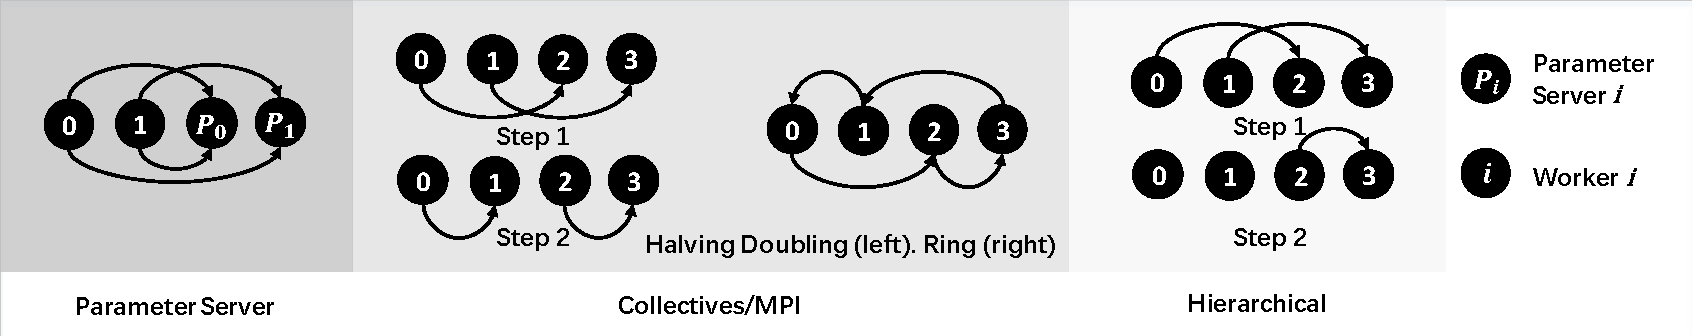
\includegraphics[width=\linewidth, trim=2 3 3 3,clip]{Figures/aggregationapproaches.pdf}
	\caption{Aggregation is commonly done with one of the three prevailing paradigms, parameter server, collectives all-reduce, and hierarchical aggregation in practice.}
	\label{fig:aggregationapproaches}
\end{figure}

\subsection{Distributed Training is Here to Stay}
Faster and more powerful accelerators (most notably TPUs~\cite{Jouppi:2017:IPA:3079856.3080246} and Nvidia DGX~\cite{AIResear61:online}) open up the possibility of training in a single device. It all of sudden seems plausible to build a ``supercomputer'' for training, which completely eliminates the need for costly communication. 

Unfortunately, building a training supercomputer does not avoid the problem of insufficient compute resources, but only delay it, for at least two reasons. From a historic perspective, it never happens that there is a surplus in the compute power when it comes to new models, as shown in Table~\ref{table:trend}: scientists can always find models whose complexities are well beyond reach of a single device, which frequently ended up being trained in a distributed fashion: the use of a single device (e.g. DGX) is not because that single device covers all the need, but rather the lack of additional devices. From an architecture perspective, compute density cannot scale forever as many hard limits are imposed on the number of transistors to fit on a fixed area, including physical effects and cooling constraints. When near these limits, it gets prohibitively difficult to build faster chips within a confined area. 

On the other hand, any training that spans device boundary, not necessarily machine boundary, can be classified as distributed training, and the communication medium need not be limited to conventional network media, but can also include device buses. With this broad view, distributed training is inherent in deep learning. In fact, many have already started looking into optimization of inter-device communication within a single machine~\cite{wang2019blink}. %at each hierarchy (GPU vs PCI-E, Node vs Ethernet), we can observe large gap between the bandwidth of communication and compute. 

\subsection{Gradient Aggregation: Common Practices}
In a loose taxonomy, collecting gradients for aggregation is commonly done with one of the following paradigms (Figure~\ref{fig:aggregationapproaches}).


\begin{figure}[t!]
	\centering
	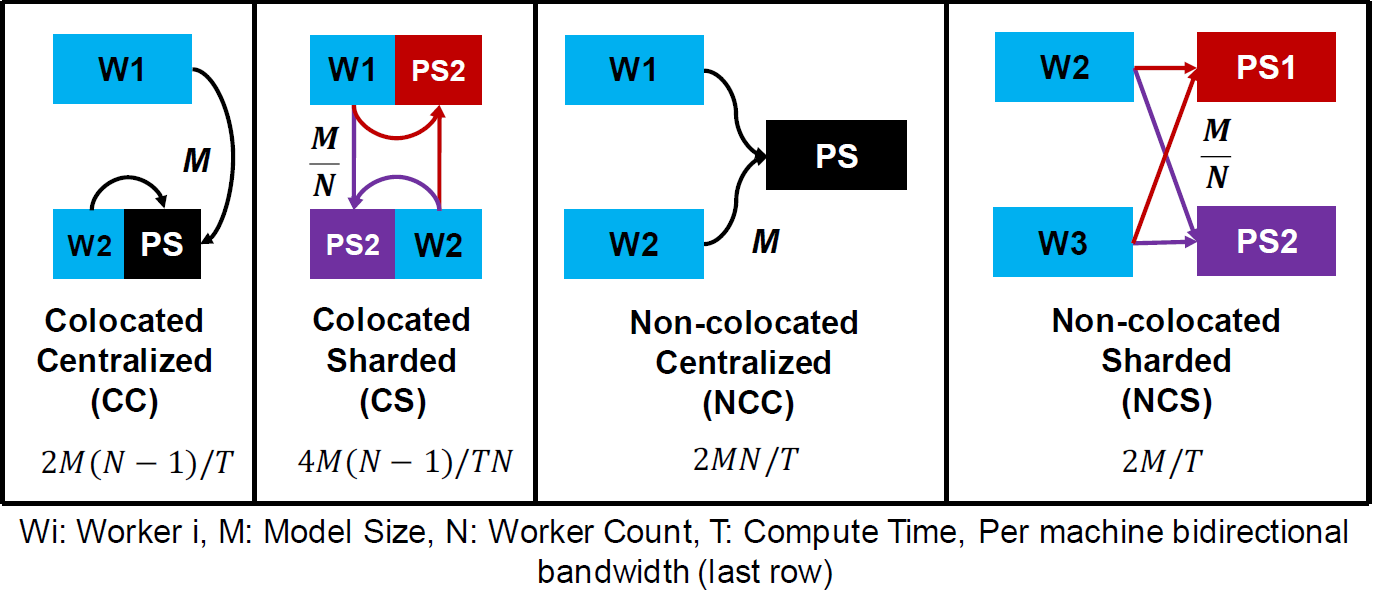
\includegraphics[width=.7\linewidth, trim=2 3 3 3,clip]{Figures/pssetups.PNG}
	\caption{Aggregation is commonly done with one of the three prevailing paradigms, parameter server, collectives all-reduce, and hierarchical aggregation in practice.}
	\label{fig:pssetups}
\end{figure}

\noindent\textbf{Parameter Servers (PS)}~\cite{ps0,ps1,ps2,ps3, phubsocc, phubsysml, poseidon,cui2016geeps}. %Nodes are assigned the role of \textit{workers} or \textit{servers}. 
PSs are key-value stores, where keys and values represent the model's layer IDs and weights. PSs can be centralized or sharded. In each iteration, all workers update the model stored in PSs with their locally-produced gradients. PS configurations primarily differ along two axes: colocated (C) versus non-colocated (NC), and centralized (C) versus sharded (S). %In a colocated setting, a PS process can run with worker processes in the same machine. In a non-colocated setting, a machine is dedicated to a worker or a PS process.  
A PS setup is colocated if a worker and a server process share the same physical machine. A PS setup is centralized if a single PS process handles all keys; and a sharded setup load-balances keys across multiple PS processes.
%A centralized PS stores the entire model, whereas each sharded PS stores only a partition of the keys in the entire key space. The size of each partition is usually balanced by the available hardware resources. 
During synchronization, each worker sends and receives model updates from each PS process. Figure \ref{fig:pssetups} illustrates the four combinations of choices from these two axes: Colocated Centralized (CC), Colocated Sharded (CS), Non-colocated Centralized (NC) and Non-colocated Sharded (NCS).

In general, sharded PSs scale better at higher hardware costs. Colocated PSs reduce total data movement on the network by $\frac{1}{N}$ with $N$ workers participating: the update for the partition of the model assigned to a colocated PS need not go through the network. While many frameworks default to CS configurations~\cite{MXNetont0:online, Distribu25:online}, in a colocated setup the PS process interferes with the training process, because both are contending for network and processing resources. Specifically, compared to NC PSs, \textit{each network interface must process roughly 2x the network traffic, because both the colocated worker and PS processes must send and receive model updates from remote hosts}, creating a major bottleneck in network-bound distributed training. 

\noindent\textbf{Collective AllReduce (CA)}~\cite{Sack:2011:SCM:2522220,Thakur:2005:OCC:2747766.2747771,collectivesOptimization,blum2000architectures,bala1995ccl}. Popular in the context of MPI, all nodes in CA participate in the communication, usually running symmetric tasks. The end goal of CA is that all nodes have a globally-reduced copy of the data. Widely used CA in training deep learning models include halving-doubling~\cite{ImageNetIn1Hour}, ring and double binary tree~\cite{Operatio73:online, Sergeev2018HorovodFA}.

Gradient aggregation can be \textit{flat} (e.g., use of PSes and CAs are generally flat) or \textit{hierarchical} (Hierarchical Aggregation, HA), which refers to the generic technique of aggregating data in multiple steps, from local to global. Exemplar usage of HA in the distributed training context include~\cite{firecaffe,choblueconnect,Geng:2018:HHP:3229543.3229544,sysmlblueconnect}, though in the context of proprietary networks. HA is highly flexible and supports mix and matching of multiple aggregation paradigms~\cite{topoawarempi, cool}.

This paper focuses on the discussion of building efficient PSs, but most of the techniques still apply to accelerating CAs as well. 

\subsection{More Efficient Distributed Training: Prior Arts}
Approaches to accelerating distributed training can be classified into one of the broad categories in the current literature.

\noindent\textbf{Synchronize less often}. One way to achieve a lower synchronization frequency is to oversubscribe GPUs. This can be done by using a very large batch size, fully utilizing GPU memories, making GPU compute the bottleneck~\cite{Nowanyon13:online, ImageNetIn1Hour, sridharan2018scaleout, jia2018highly}. Large batch sizes reduce communication frequency. However, this eliminates the potential of achieving a larger speedup with a fast communication plane. For example, with ResNet-50, ~\cite{Shen2018NexusA} shows only 10 samples are needed to fully utilize a recent GPU. This means the computation of large batches can be further spread to more GPUs, provided that communication overhead is low. Further, large batch optimization is also not universally available (requiring GPUs with large memory) and may be subject to worse generalization~\cite{keskar2016large}.

Orthogonal to large batch optimization, another line of work target at less synchronization tunes the consistency model of distributed training, with relaxed consistency~\cite{DBLP:journals/corr/DaiKWHGX14,SSP,BSP,Wei:2015:MCC:2806777.2806778,Litz,xie2018orpheus,wang2018adaptive}. Generally, these relaxed consistency models do not mandate a strict barrier for synchronization at iteration granularity, and instead, allows for staleness in the model and a potential different view of model from each worker, removing the synchronization overhead from the critical path. However, these methods suffer from difficulty in reproducing the models. 

\noindent\textbf{Send less data}. Sending less data accelerates distributed training in a bandwidth-bound environment, and can be achieved through (1) lossless compression~\cite{burtscher2009fpc}; (2) lossy compression, removing redundancy in the SGD algorithm~\cite{lin2017deep}; (3) quantizing update gradients to low bit representations and locally apply residual errors~\cite{cntk1bt, lim20183lc} and (4) decomposing large update matrices~\cite{projectAdam,poseidon,xie2015distributed} and reconstructing at destination. These methods either trade more computation for less communication, or risk affecting the final convergence accuracy of the model, and both of which may turn out \textit{increasing} the total wall clock time required to reach the target accuracy.

\noindent\textbf{Build faster clusters}. Another series of work involves building specialized hardware clusters for distributed training with quick interconnects to tackle communication bottlenecks~\cite{DBLP:journals/corr/abs-1711-00489, You:2018:ITM:3225058.3225069, DBLP:journals/corr/abs-1711-04325,jia2018highly,DBLP:journals/corr/abs-1811-05233,sun2019optimizing, ImageNetIn1Hour, firecaffe}. While the results have been encouraging, these approaches demand steep investments and are not available to everyone.

\noindent\textbf{Hide communication latency}. Most modern frameworks encode the model being trained as a dataflow graph. An operator is executed as soon as its dependencies are resolved, and this allows overlapping of communication and computation during the backpropagation stage of distributed training. Some work even attempt to reprioritize sending of first layers over later layers to deal with this priority inversion problem. Notable applications of this idea include~\cite{hashemi2018tictac, prioritybased, poseidon, 10.1145/3341301.3359642}. However, communication latency hiding has severe limits: faster computation device leaves smaller room; many model training is in fact bandwidth bound, and hiding latency only has limited impact on the total training time.

\noindent\textbf{Use finer grain parallelism}. This can be done by blending in higher compute hardware utilization of data parallelism and lower communication cost of model parallelism to form pipelined parallelism~\cite{harlap2018pipedream}. This can also be done by allowing a flexible combination of slicing along arbitrary dimensions of S(ample)O(perator)A(ttribute)P(arameter), which enables more execution possibilities, effectively enlarge the action space. More efficient schedule can then be determined by intelligently searching through the enlarged space by taking communication cost into account~\cite{jia2018beyond}. However, these methods have the limit of needing to research as soon as the underlying hardware environment, or the models being trained change.

\noindent\textbf{Accelerate at network level}. The emergence of programmable network devices open up the opportunity to accelerate distributed training at the core of network, allowing gradient aggregation in the network devices, resulting in lower parameter exchange latency and lower bandwidth requirement (e.g. broadcast of aggregated model can be efficiently done with a network switch~\cite{sapio2019scaling,luomotivating}). Current programmable devices are not without limits, enforcing hard constraints on compute and memory.

\noindent\textbf{Codesign software with hardware, cluster, network and environment}. This is the approach where the software stack is codesigned with underlying hardware, cluster, physical network and environment, based on the observation that existing software stack does not take important factors (such as underlying hardware, the topology of the physical network, and the shared environments of the commercial clouds) into consideration. Examples of this approach include \plink{}~\cite{phubsocc, phubsysml}.

\noindent\textbf{Improving cluster-level efficiency}. A series of work ~\cite{222611,Shen2018NexusA} target at an orthogonal goal, and instead of optimizing for each individual task, they aim to achieve an average high utilization of compute resources in a cluster, by time-sharing (preemption) and better placement etc.

\begin{figure}[t!]
	\centering
	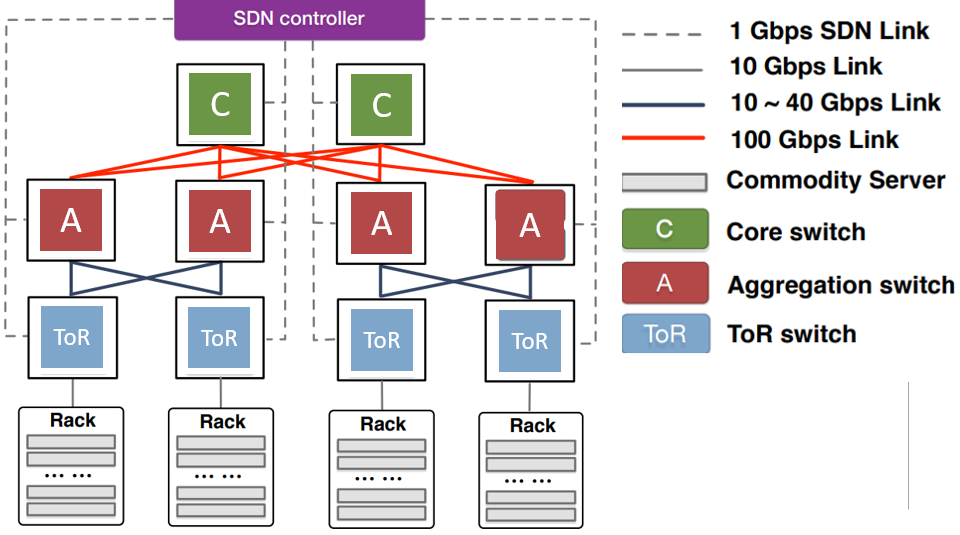
\includegraphics[width=.6\linewidth, trim=2 3 3 3,clip]{Figures/dc.png}
	\caption{Overview of a typical datacenter network topology.}
	\label{fig:dc}
\end{figure}

\subsection{Datacenter Network Toplogy}
\label{sec:datacenternetwork}
A typical datacenter network has a hierarchical, multi-tiered topology~\cite{Mysore2009PortLandAS,VL2,Roy2015InsideTS,incbricks} (Figure~\ref{fig:dc}). Machines are grouped into \textit{racks}, each connecting to a top-of-rack \textit{(ToR)} switch. ToR switches are connected to multiple upper level devices. In this setting, the communication performance of two end-hosts is affected by where they reside: they enjoy full link bisection bandwidth within a rack, because link capacity is not shared at the rack-level, but if they are on different racks, the communication performance depends on link congestion and oversubscription ratio~\cite{Bilal2012ACS}. In this paper, we use \textit{locality} to refer to the cause of variation in communication performance, which includes: (1) physical topology: the location of the nodes and (2) dynamic network load. Efficient communication requires carefully architecting software to tap into both aspects~\cite{eyeQ, 27Octobe15:online}: solutions that ignore physical topology are subject to long-term communication imbalances, and those that ignore dynamic network load suffer from short-term inefficiencies.
\chapter{\pbox: a Balanced Hardware Design for Parameter Servers at Rack-Scale}
\label{sec:phub}
We now describe \pbox, the solution to inefficient distributed training for clusters with a flat network topology (rack-level). \pbox provides a re-design of a PS at the hardware level, and mostly applies to situations where the user assumes full control over the cluster. We start with the current problem with the PS software and hardware that runs it. When deployed, \pbox serves as a centeralized parameter server in the cluster.

\begin{table}
        \centering
        \footnotesize
	\begin{tabular}{|c|c|c|c|c|}
		\hline
		Network   & CC & CS & NCC & NCS\\
		\hline
		ResNet 269    & 122   & 31   & 140    &  17   \\
		\hline
		Inception & 44   &  11  &  50   &  6  \\
		\hline
		GoogleNet & 40   &  10  &  46   &  6  \\
	
		\hline 
		AlexNet   & 1232  &  308  & 1408    &  176  \\
		\hline
	\end{tabular}
	\caption{Estimated bisection bandwidth (Gbps) lower bound on the PS side for hiding communication latency in a small cluster of 8 nodes with GTX 1080 Ti.}
	\label{table:bwReqDC}
\end{table}

\section{Insufficient Bandwidth and Overprovisioned Compute Resources in Rack-Scale Clusters}
Centralized PSs have lower cost than NCS PSs, and half of the bandwidth stress compared to CS PSs on each interface card. Thus it is desirable to have a centralized reduction entity at rack level. However, scaling a centralized PS to rack scale is challenging~\cite{firecaffe}.
%Because they dedicate their full bandwidth to the PS process, centralized PSs are bandwidth efficient without the extra hardware cost for non-colocated sharded PSs. They are also compute efficient when not overwhelmed~\cite{firecaffe}. However, while optimizations in \mysection\ref{sec:commonOptimizations} benefit sharded servers, they have only limited effect on the throughput of a centralized PS. 
%The root cause is hardware imbalance in resource allocation of the host machine.
The root cause is hardware imbalance in the allocation of computation and communication resources in the host: centralized PSs usually run on the same hardware configuration as a worker, which have only one or two network interfaces. This implies incast congestion from their high bandwidth usage when serving multiple workers, starving the compute units. We profiled the training of multiple DNNs of different model sizes and computation-to-communication ratios. Our setup used 8 workers and 8 CS PSs. We observed \textit{it was nearly impossible to eliminate communication latency in cloud-based training due to limited network bandwidth.} We estimated the minimum bandwidth requirement to fully hide communication latency in the network as follows: given a model size of $M$, and $T$ time for each iteration, with $N$ workers participating, the network should at least be able to send and receive model updates within the computation time (assuming infinitely fast PSs and that sending/receiving could fully overlap). Figure \ref{fig:pssetups} gives an analytical lower bound of \textit{per host bandwidth}, and Table \ref{table:bwReqDC} shows the required bandwidth for various DNNs: DNNs demand more bandwidth than mainstream offers (typically 10 Gbps). 

%Hardware imbalances result from vastly different computation and communication resources in a machine, which is in turn related to how centralized PSs are deployed. Centralized PSs usually run on the same hardware as a worker and have only one or two network interfaces. This implies incast congestion from their high bandwidth usage (Table \ref{table:bwReqDC}) when serving multiple workers, starving the compute units. 

%Existing frameworks also cannot efficiently use full hardware, even if multiple interfaces are present (for example, TensorfFlow and \mxnet can only use multiple interfaces by spawning multiple PS processes), let alone understanding the topology of the underlying hardware to balance workload in each interface, processor core and NUMA domain.

One trivial solution would be to simply use interfaces with higher bandwidth. However, even in the best case, a single network interface is not capable of saturating memory or PCIe bandwidth. A single network interface also causes serialization delay and further imbalance across NUMA domains in a typical server. %It is not possible to fully utilize the entire server without balancing these resources.

%The solution may seem trivial: just add more interfaces, or use interfaces with higher capacity. These, however, are not enough. First, most parameter server implementations (TensorFlow, \mxnet and etc) do not allow use of multiple interfaces in a single parameter server process instance. To support that, the software stack must understand the topology of the underlying system and produce a balanced scheme across multiple interfaces with minimum polling overhead; second, existing single interface is unlikely able to match the memory bandwidth nor the PCIe bandwidth, and they can still cause serialization delay, further causing imbalance across NUMA domains on typical server systems.

%Software changes alone is not enough to scale training throughput on a typical centralized parameter server, because the hardware offered is inbalanced itself: the provisioned network bandwidth is vastly smaller than available memory bandwidth.
%Therefore, a hardware design that optimizes balance is needed to fully scale a centralized PS. 

\section{\pbox Architecture}
This section describes \pbox, our \textit{balanced parameter exchange system}. We maintain that a centralized system, when architected properly, can provide high throughput, low latency, sufficient scalability for a rack, and low cost. We focus on the hardware side of \pbox, and in the next section, we detail the software side.

We prototyped \pbox using an off-the-shelf server platform that was configured to our requirements. Our goal was to balance IO and memory bandwidth; our prototype system had memory bandwidth of 120 GB/s and theoretical overall bidirectional IO bandwidth of 140 GB/s. To fully utilize resources, \pbox needed a matching network capability, which we provided by using multiple network interfaces. Figure \ref{fig:phub} shows the resulting \pbox design. The system includes 10 network interfaces, each of 56 Gbps link speed, connected to a switch. This uses all PCIe bandwidth on our dual socket prototype and provides roughly 136 GB/s bandwidth once IB and PCIe framing overheads are taken into account, balancing IO and memory bandwidth.

\begin{figure}[t!]
	\centering
	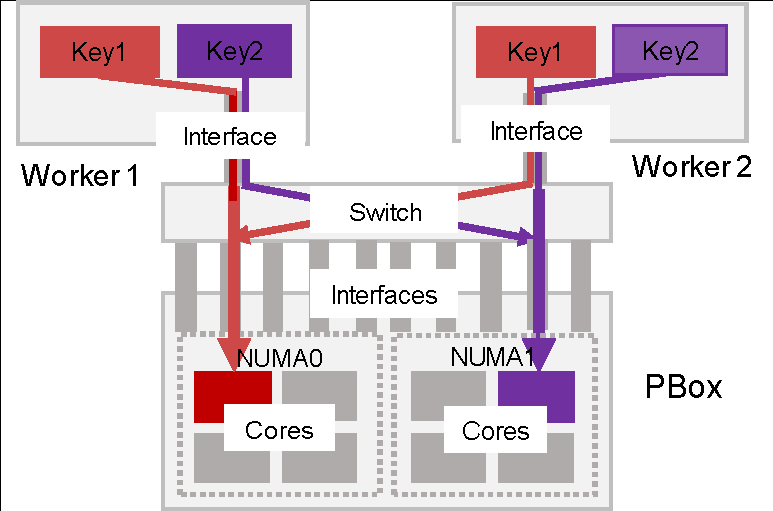
\includegraphics[width=.6\linewidth,trim=2 1 1 1,clip]{Figures/PHubOverview.pdf}
	\caption{The \pbox architecture}
	\label{fig:phub}
\end{figure}



\begin{figure}[t!]
	\centering
	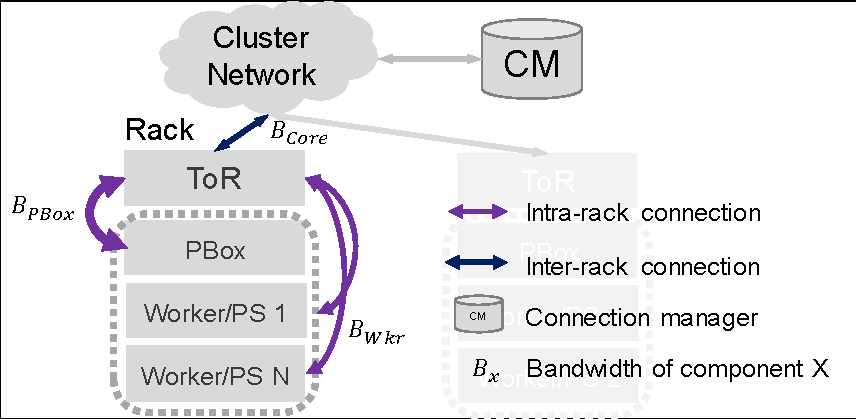
\includegraphics[width=.6\linewidth,trim=3 1 1 2,clip]{Figures/PBoxDeployment.pdf}
	\caption{\pbox deployment scheme}
	\label{fig:pBoxDeployment}
\end{figure}


\section{Multi-Rack Deployment and Topology-Aware Reduction}
\label{sec:hierarchicalReduction}
When needed, \pbox can be used to upscale distributed training to datacenter levels. To extend service coverage of a single \pbox device, we associate a \pbox with a ToR during deployment, for two reasons. First, full bisection bandwidth is achievable for machines in the same rack, making it ideal for a central reduction entity as \pbox, while oversubscription occurs between the ToR and the cluster network. Second, as we show later, a single \pbox has enough scalability for a typical rack of worker machines.

When provisioned in each rack (Figure \ref{fig:pBoxDeployment}), \pbox{}es can form an array of sharded PSs, or run a \textit{hierarchical reduction} algorithm for a training task that spans multiple racks through the coordination of a connection manager. Hierarchical reduction works in three steps: first, each \pbox centrally aggregates gradient updates from workers in the same rack; then, the \pbox{} nodes start cross-rack aggregation and compute globally aggregated gradients; finally, each per-rack \pbox runs an optimizer on this gradient and broadcasts the new weights back to local workers.

Hierarchical reduction trades off more rounds of communication for lower cross-rack traffic ($1/N$ with N-worker racks). We can determine when hierarchical reduction is potentially beneficial with the simple model below:
%\[	max(\frac{N-1}{B_{bn}}, \frac{1}{B_{Wkr}})  > max(\frac{1}{B_{Wkr}}, \frac{N}{B_{PBox}}) + C\]

\begin{align*}
	 \frac{N(R-1)}{RB_{Core}} >  max(\frac{N}{B_{PBox}}, \frac{1}{B_{Wkr}}) + C
\end{align*}
%\[\]

where $B_{PBox}, B_{Core}$ and $B_{Wkr}$ are the bandwidths of a \pbox, the network core, and a worker, and $R$ is the number of racks. When the condition is true, this means the time to perform cross-rack transfer is larger than the added latency of a two-level reduction, which consists of a per-rack local aggregation that happens in parallel and an inter-rack communication (with cost $C$) done with either sharded PSs ($C=\frac{r-1}{rB_{bn}}$, where $B_{bn} = min(B_{PBox}, B_{Core})$) or a collectives operation (e.g., $C\approx\frac{r-1}{rB_{bn}}$ with racks forming a ring). $C$ can be directly measured, and $B_{Core}$ can be effectively probed by using~\cite{hu2002estimating,hu2003evaluation}.

\chapter{\phub: Streamlined Software Stack for Rack-Scale PSs}

\begin{table}[tb!]
        \centering
        \footnotesize
	\begin{tabular}{|c|c|c|c|c|}
		\hline
		   & Local & 2 nodes & 4 nodes & 8 nodes\\
		\hline 
		TensorFlow   & 152  &  213  & 410    &  634 \\
		\hline
		Caffe2 & 195   &  266  &  343   &   513  \\
		\hline
		TF+Poseidon\cite{poseidon} & 209 & 229  & 364 & $<$648 \\
		\hline
		MxNet & 190  &  187  &  375   &  \textbf{688}  \\
		\hline
	\end{tabular}
	\caption{Throughput (samples/s) of training ResNet 50 on  major DNN training frameworks with a 56 Gbps network.}
	\label{table:frameworkPerf}
\end{table}

\begin{figure*}
    \centering
	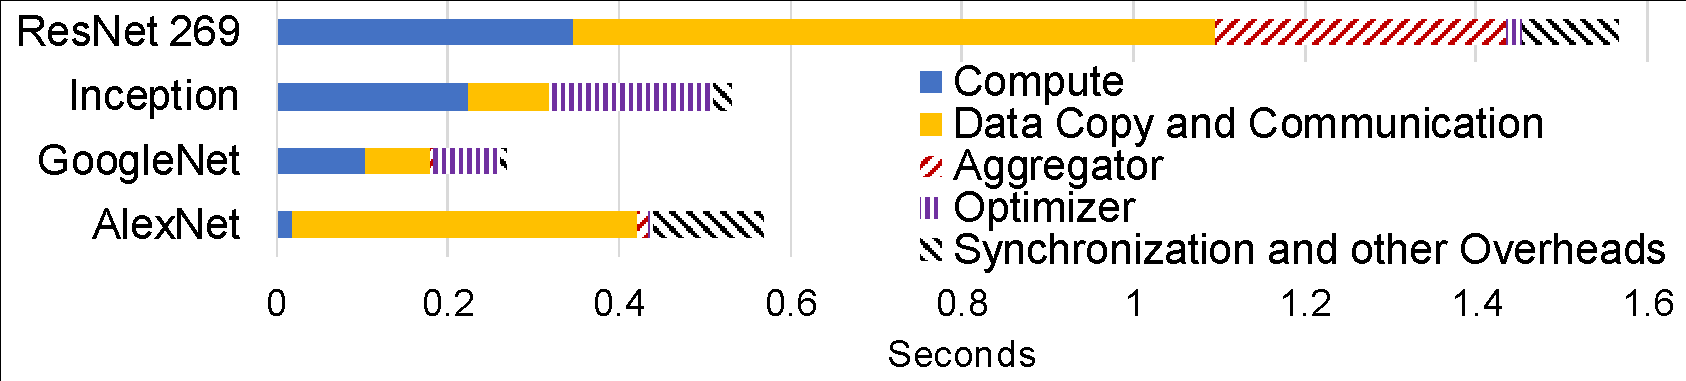
\includegraphics[width=.7\linewidth,trim=3 2 2 4,clip]{Figures/OverheadBreakdown.pdf}
	\caption{Progressive overhead breakdown of different stages during the distributed training pipeline for MxNet distributed training on a 56Gbps network. Link capacity accounts for a small fraction of the copy and communication overhead in this setting.}
	\label{fig:overheadBreakdown}
\end{figure*}

Hardware alone solves only part of the problem. Existing frameworks cannot efficiently use the full hardware capability of \pbox (for example, TensorFlow and MxNet support multiple interfaces only by spawning multiple PS processes). The result is, even with ample communication resources, existing PSs failed to hide communication latency and struggled to scale. Table \ref{table:frameworkPerf} shows that all major DNN training frameworks %failed to achieve 50\% scaling on a 56Gbps IPoIB network (112Gbps bidirectional) in our cluster with 8 workers and PSs. 
do not scale well with a 56 Gbps IPoIB network.

\section{Inefficient Software Stack}

We investigated the cause for MxNet by breaking down the overhead for each major component of a training iteration (legends of Figure \ref{fig:overheadBreakdown}). Since all stages overlap one another, and since ideally we would like early stages to fully hide the latency of later stages, we show \textit{progressive overhead} in Figure \ref{fig:overheadBreakdown}: we gradually turned on different components in the MxNet distributed training pipeline, and each segment shows the \textit{additional overhead that previous stages could not hide}. Specifically, the compute segment shows how long the GPU is active; the data copy segment shows the additional overhead of turning on distributed training without aggregation and optimization; the aggregation and optimization segments show additional overheads of enabling them in that order; and the ``other'' overheads segment includes synchronization and overheads that are not specific to a single component. We explain the overhead for some components:

%\begin{CompactItemize}
	\noindent\textbf{Data copy:} each layer's parameters were copied to and from OS buffers 4 times during parameter exchange.
\vspace{-0.1ex}	

	\noindent \textbf{Aggregation and optimization:} MxNet's approach to achieving parallelism in these operations did not achieve high throughput in our measurements.
\vspace{-0.1ex}	
	
	\noindent \textbf{Synchronization:} MxNet's dispatcher thread needs to synchronize access with ZMQ threads, aggregation threads and an optimization thread via shared queues, leading to bad locality and increased synchronization overhead. 
	
	
\section{\phub Software}
Based on above findings, we propose \phub, an optimized PS implementation that reduces framework overhead with software optimizations. With \phub, we aim to:

% we rearchitected the PS to optimize the network stack, provide efficient gradient aggregation and optimization, and streamline the approach to sending and receiving gradients and model parameters. We also designed \phub to be a rack-scale parameter service, which allows job sharing and topology-aware reduction algorithms.

\begin{enumerate}[noitemsep,topsep=0pt,parsep=0pt,partopsep=0pt]
\item Minimize gradient/model communication overhead.
%\item Gradient data should be laid out to exploit locality and enable overlap.
%\item Preserve locality and enable overlap of gradient processing and receiving.
\item Enable efficient gradient processing and overlap with communication.
\end{enumerate}

We now software optimizations that benefit different stages in distributed training across all common PS configurations. % the network stack optimization, gradient aggregation and optimization, fine-grained key chunking, and chunk-to-core mapping. These software optimizations benefit common PS setups.

\subsection{Network Stack Optimizations}
\label{sec:IBOptimization}
%We sought a solution that enabled zero-copy and kernel bypass for minimal latency and overhead when moving data. 
We sought to mitigate data movement latency with zero-copy and kernel bypass. We chose InfiniBand (IB) since we were already familiar with the Verbs API, and it is available in major cloud providers~\cite{AzureWin5:online}. Note that similar results could be achieved over Ethernet using RoCE, DPDK or other frameworks. We followed the guidelines from~\cite{rdma}; we tried two and one-sided RDMA, and two-sided send/receive operations and found similar performance in our workload. We briefly highlight some implementation details:

\noindent \textbf{Minimal Copy:} Leveraging InfiniBand's zero-copy capability, the only required data copy is between the GPU and main memory. When one GPU is used, this can be eliminated with GPU-Direct RDMA on supported devices.

\noindent \textbf{NUMA-Aware, One-shot Memory Region Registration:} Since a worker can operate on only one model update at a time, it is sufficient to allocate one read buffer (for the current model) and one write buffer (for update reception) for the model. To minimize InfiniBand cache misses, \phub preallocates all buffers in the NUMA domain where the card resides as a contiguous block.

\noindent \textbf{Minimal Metadata:} To maximize bandwidth utilization and minimize parsing overhead, \phub encodes metadata (such as callback ID and message opcode) into InfiniBand's queue pair number and immediate field. This saves \phub an additional PCIe round trip (from IB send scatter/gather) to gather metadata when sending messages.

%\phub leverages InfiniBand's zero-copy ability to reduce copies from the network to  GPU memory by re a per-key aggregation buffer set up during \code{Initialize}; the buffer aggregates gradients from multiple devices before pushing them out to the network. Thus, the only remaining copy to the buffer is from the GPU. For a single GPU, this copy can be eliminated using  GPU-Direct RDMA on supported devices. Before \phub uses InfiniBand as its data plane, it must register all memory used for communication. A worker can have only one model update executing concurrently. Thus, it is sufficient to allocate and register a buffer per worker for gradient reception, and a single buffer for the model. To minimize InfiniBand card memory registration cache misses, \phub pre-allocates all buffers to a single contiguous memory region that it registers. \phub memory registration is NUMA-aware. Memory is allocated on the same NUMA domain where the card resides to reduce QPI traffic between sockets. To keep track of pending operations, some metadata is required, such as current message meaning, sender and receiver information, opcode, and a timestamp used to execute the proper callback. To maximize bandwidth utilization, we encode all metadata into InfiniBand's queue pair number or immediate field. We also designed timestamps to be logical and deterministic, so they can be calculated by combining a global batch number with  message's key. This saves us an additional PCIe round trip (from IB send scatter/gather) to gather metadata when sending messages. 

\subsection{Gradient Aggregation and Optimization}
\label{sec:tallvswide}


% for 2690v4: AVX max speed is 2.1 GHz, 1 256-bit add per cycle (2 if FMA multiplying by 1, but that's annoying)
% so 2.1 GHz * 8-float vectors (32 bits) * (2 reads + 1 write) * 28 cores
% so 470 billion ops/second, 5645 GB/s bidir for 2 read 1 write, 1882 GB/s if aggregation buffers (1read, 1write) are in cache
%% Gradient aggregation could be performed on the CPU or GPU. Here, we posit that the CPU is sufficient for this job.
%% Aggregation is simply vector addition: we read two floats and write one back.
%% For modern CPUs, this is fast: if we keep the processors' AVX ALUs fed, we can perform 470 single-precision giga-adds per second, requiring 5.6TB/s of load/store bandwidth.
%% A typical dual socket server can sustain up to 140GB/s memory bandwidth. 5.6TB/s is impractical for the large vectors involved in DNN training workloads, making aggregation inherently memory bound. There is thus little point in copying gradients to GPU to perform aggregation.
Gradient aggregation could occur in the CPU or GPU~\cite{GeePS}. Here, we posit that the CPU is sufficient for this job.
Aggregation is simply vector addition: we read two floats and write one back.
%Our evaluation hardware is typical of modern dual socket servers. 
With our typical modern dual socket server, if we keep our processors' AVX ALUs fed, we can perform 470 single-precision giga-adds per second, requiring 5.6 TB/s of load/store bandwidth.
But the processors can sustain only 120 GB/s of DRAM bandwidth, making aggregation inherently memory bound. Thus, copying gradients to a GPU for aggregation is not helpful.

\begin{figure}[t!]
    \centering
	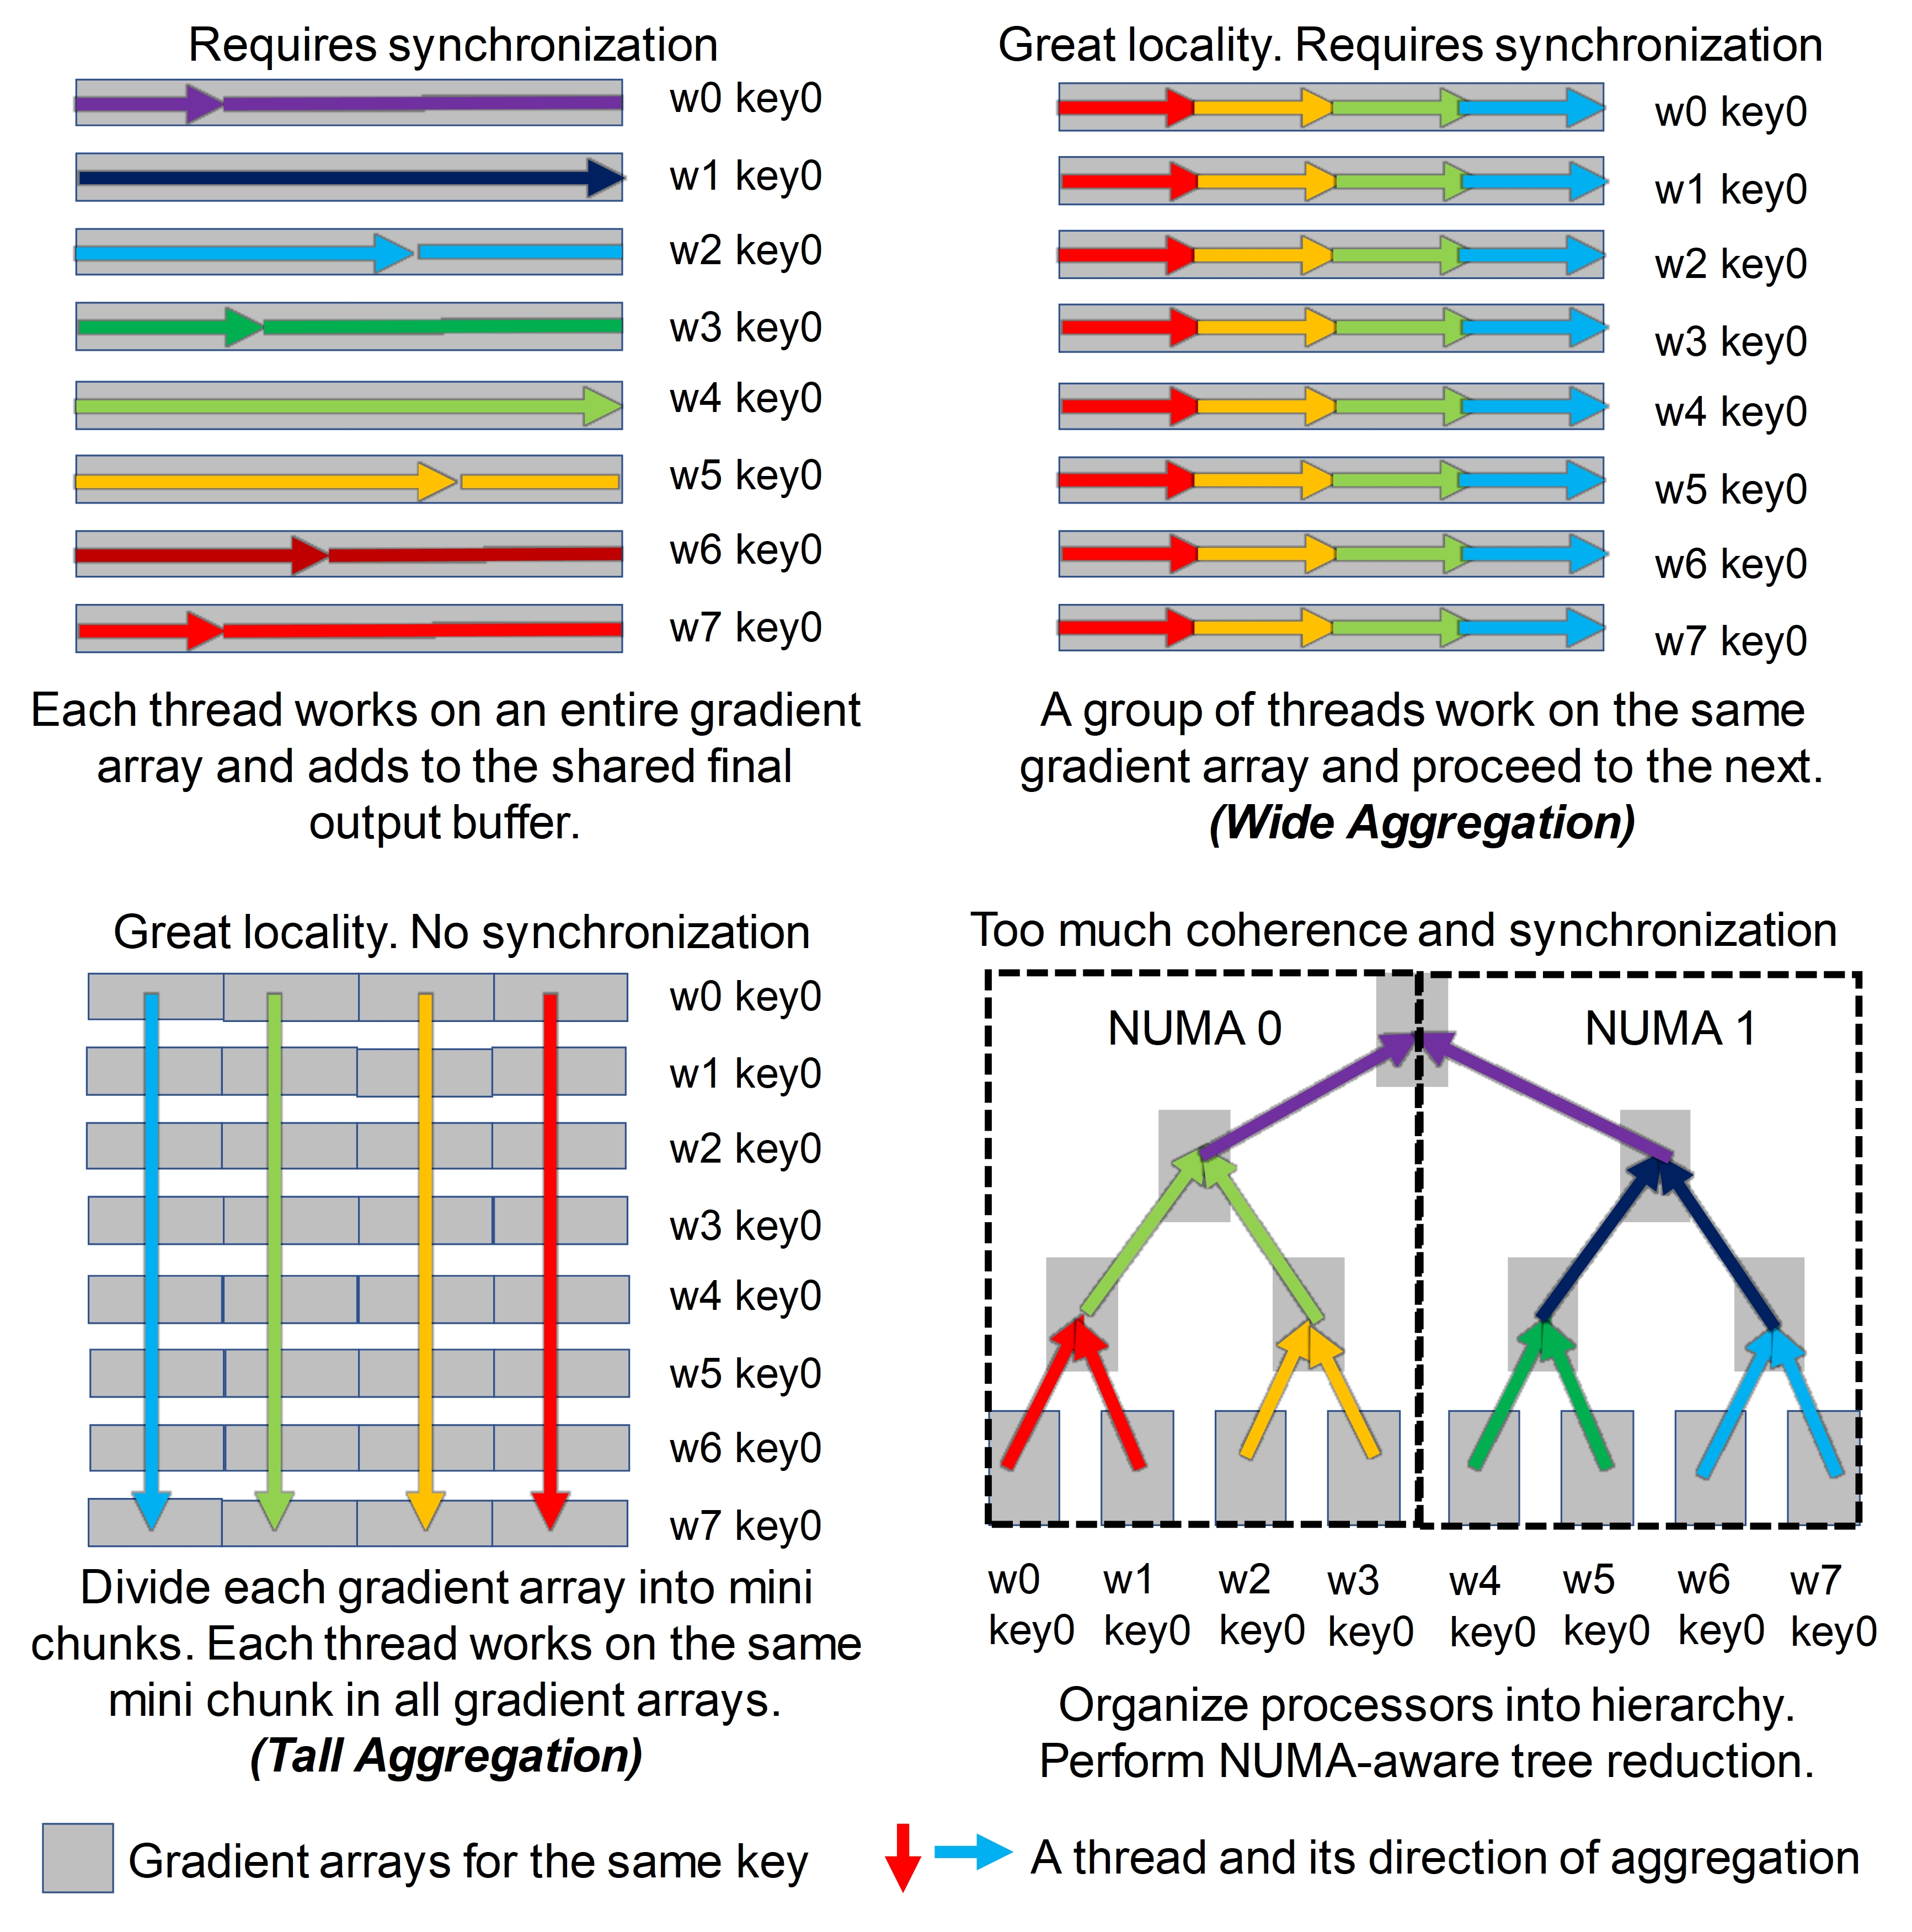
\includegraphics[width=.7\linewidth,trim=5 5 15 5,clip]{Figures/AggregationExperiments.jpg}
	\caption{Ways of gradient aggregation. A thread (arrow) aggregates over the array (gray rectangle) of gradients from a worker. }
	\label{fig:gradientAggregation}
\end{figure}


There are many ways to organize threads to perform aggregation.
%We start with the case where all workers' gradient arrays for a given key are received. 
Figure \ref{fig:gradientAggregation} shows four options we prototyped, assuming gradient arrays are available at once. We found that the best performance was achieved using the two discussed below; other schemes suffered from too much synchronization overhead, poor locality and/or high latency.

\textit{Wide aggregation} is typical to systems like MxNet that call BLAS routines for linear algebra. In these systems, a group of aggregation threads process one gradient array at a time; each thread works on a partition of that array. 
%When the current array is done, the group moves to the next.

A variation of wide aggregation is \textit{tall aggregation}, which chunks a gradient array into mini-chunks of predefined sizes; each thread works independently to process the same chunk across all gradient arrays for a given key. This is the preferable way to organize threads for many reasons.
First, gradient arrays do not arrive instantly. For a large key (e.g., a fully connected layer), aggregation and optimization cannot start for wide aggregation until the key is fully received; for tall aggregation, the process can start as soon as the first chunk is received.
Second, in wide aggregation, it is challenging to balance the number of threads dedicated to aggregation and to optimization, let alone partitioning threads to work on different keys since they can arrive at the same time; %, as the optimal assignment can be DNN dependent; 
thread assignment for tall aggregation is natural.
Third, wide aggregation induces queuing delays: it effectively processes one key at a time versus tall aggregation's many ``mini-queues.''
Fourth, wide aggregation puts many threads to work in lock-step on pieces of data, which incurs non-trivial synchronization overhead; tall aggregation requires no coordination of threads as aggregation is an element-wise operation.

%and tall aggregation allows aggregation to start as soon as a chunk is received, without waiting for the entire gradient array to arrive (some networks have large fully connected layers of size up to tens of megabytes), overlapping communication and computation. More importantly, it is challenging to balance the number of threads that are dedicated to aggregation and optimization if they overlap. 

%Tall aggregation essentially creates many mini queues, alleviating queueing delays. Wide aggregation approach on the other hand, can incur high overhead from repeated thread coordination, and working on only one gradient (which belongs to the same key) at a time effectively forms a queue causing delays. Furthermore, the optimal value for number of threads is workload dependent in wide aggregation. Figure \ref{fig:tallVSWide} compares these two approaches. We chose tall aggregation in \phub.

\phub tracks the number of currently aggregated mini-chunks for a given key. When a chunk is received from all workers, it can be optimized. This step is natural in \phub: the thread that aggregates a particular chunk also optimizes that chunk. As a result, \phub{}'s aggregation and optimization scheme effectively maps a particular chunk to a single core (since \phub pins threads to cores). On the other hand, MxNet uses wide optimization: when a key is fully aggregated, another set of threads is launched to perform aggregation. No overlap occurs between key aggregation and optimization. 
%% \phub tracks the number of currently aggregated chunks for a given key.
%% \phub counts the number of workers for which it has aggregated a chunk.
%% When a chunk has been received from all workers, it can be optimized.
%% This step is natural in \phub: the thread that aggregates a particular chunk also performs optimization for that chunk.
%% As a result, \phub{}'s aggregation and optimization scheme effectively maps a particular chunk to a single core.
%% Conversely, MxNet uses wide optimization: when a key is fully aggregated, a new set of parallel tasks is launched to perform optimization.
%% No overlap occurs between the two steps. Figure \ref{fig:tallVSWide} compares throughput of tall and wide aggregation in \phub and MxNet: tall aggregation/optimization outperforms their wide counterparts.


%Similar to gradient aggregation, optimizer is another element-wise step. \phub naturally assign optimization task of each mini chunk of a key to the core that is responsible for its aggregation (tall optimization). This allows optimization and aggregation of a same key to overlap\footnote{As a side note, MxNet uses wide optimization as well. When a key is fully aggregated, it moves to the optimization stage and potentially another group of threads is launched. There is no overlapping between key aggregation and optimization.}.

%% We implemented two variants of each optimizer: one that uses normal cached loads and stores, and one that bypasses the caches with non-temporal prefetches and stores. This allowed us to test whether caching only the model or gradients wold provide a benefit. We found the temporal version to be more effective. \phub{}'s aggregators and optimizers are fully extensible: implementations that comply with \phub{}'s API can be used during runtime.

We explored the benefits of caching by implementing two variants of each aggregator and optimizer: one using normal cached loads and stores, and one with non-temporal prefetches and stores. We found it beneficial to cache both the model and gradients. \phub{}'s aggregators and optimizers are fully extensible: implementations that comply with \phub{}'s API can be used during runtime.

\subsection{Fine-grained Key Chunking}
%\phub chunks key for two purposes. First, fine-grained key chunking lets \phub balance server and processor core load. This is important because different neural network layers can have significantly different total weight sizes, from a few bytes to tens of MBs. Second, fine-grained key chunking supports tall aggregation and optimization, so processor cores can be fully utilized.

%This makes balancing server and processor core load challenging. By chunking the weight size into a series of virtual layers (a set of virtual keys) of small, fixed size, \phub can balance load of processor cores optimally.These virtual keys are then treated independently in model update; \phub relies on fined grained key chunking to support tall aggregation and optimization, usually at the size of a few to tens of kilobytes.

Chunking in \phub differs from other systems in key ways. Initially, our goal is to balance load at a fine-grained level across cores and interfaces rather than across server shards: chunking is turned on even when a centralized PS is used. Next, we would expect our optimal chunk size to be the smallest message size that can saturate network bandwidth, whereas systems like MxNet prefer larger key chunk sizes to avoid excessive thread synchronization overhead.
%In fact, \phub defaults to 32KB of chunk, while MxNet defaults to a 4MB chunk size.
In fact, \phub's default is 32KB, while MxNet's is 4MB.
Finally, key chunking enables another important optimization: the overlapping of gradient transmission with aggregation and optimization. Aggregation starts only after a key's entire gradient array is received; and for large layers, this adds significant delay. With small key chunks, \phub enables ``streaming'' aggregation and optimization.

\begin{figure}[t!]
	\centering
	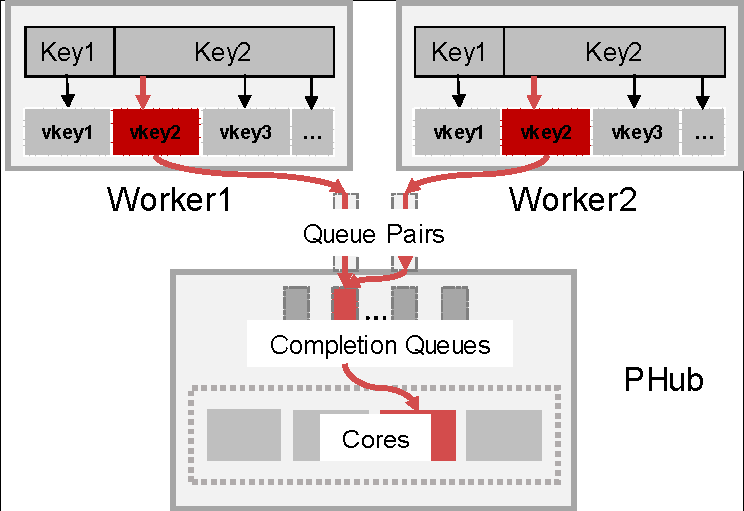
\includegraphics[width=.5\linewidth,trim=1 1 1 1,clip]{Figures/MappingChunkToCore.pdf}
	\caption{The process of mapping a chunk to a core in \phub using fine grained key chunking. Keys are chunked into virtual keys. The highlighted key is delivered to a highlighted (fixed) core through a highlighted (fixed) queue pair and completion queue. }
	\label{fig:mappingChunkToCore}
\end{figure}


\subsection{Mapping a Chunk to a Core}
\label{sec:chunk2core}
\phub's assignment of chunks to cores is computed during initialization. At that time, the set of all keys is sharded across the cores and interfaces available on PS nodes.
A specific chunk is always directed to a particular queue pair,
which is associated with a shared completion queue on the chunk's core.
%the responsible core has a single completion queue for all its associated queue paris.
%which is associated with a completion queue and is eventually processed by that single core.
All message transmission, reception, and processing for that chunk is done on that core. Cores do not synchronize with each other. Once processed, a chunk is transmitted back to the workers on its originating path. The worker side of \phub assembles and disassembles a key, a process that is transparent to the framework.

\phub{}'s chunk assignment scheme provides significant locality benefits. The same key likely arrives around the same time from multiple workers; the associated aggregation buffer is reused during this period. The scheme also encourages locality in the InfiniBand interface in the queue pair and memory registration caches. %, which can further benefit performance.

This scheme imposes challenges in balancing load across cores, queue pairs and completion queues. \phub uses a 4/3 approximation set partition algorithm to balance each component's workload at each level, which produces practically balanced assignments in our experiments. \phub{}'s chunk mapping mechanism is summarized in Figure \ref{fig:mappingChunkToCore}.

\section{The \phub Service API and Interoperability with other Frameworks}
\phub{}'s API is designed for compatibility with multiple DNN training frameworks. Workers use \phub by first calling \code{PHub::CreateService} on the connection manager. This sets up access control and a namespace for the training job and returns a handle. The client side uses the handle to finish setup. \phub uses the namespace and an associated nonce for isolation and access control. 

Jobs call \code{PHub::ConnectService} to rendezvous servers and workers, exchanging addresses for communication. This call replaces \code{Van::Connect} in MxNet, \code{Context::connectFullMesh} in Caffe2 and \code{GrpcServer::Init} in TensorFlow. \code{PHub::InitService} causes the current \phub instance to allocate and register receive and merge buffers. \phub also authenticates each worker's identity using the nonce. Authentication is a one-time overhead and once a connection is established, \phub assumes the remote identity associated with that address/port/queue number does not change during training.

\phub{}'s functional APIs include standard synchronous or asynchronous \code{PHub::Push/Pull} operations that are used in TensorFlow (\code{GraphMgr::SendInputs/RecvOutputs}) and MxNet (\code{KVStoreDist::PushImpl/PullImpl}). \phub also includes a fused \code{PHub::PushPull} operation that perform a push, waits until all pushes are complete, and pulls the latest model. The fused operation often saves a network round-trip as push and pulls are frequently issued consecutively. This operator can serve as a drop-in replacement for Caffe2's \code{Algorithm::Run}.


\section{Interaction of \pbox and \phub}
\phub takes full advantage of \pbox by extending the chunk-to-core mapping scheme%It ensures balance across queue pairs, completion queues, interfaces, cores, and NUMA domains. 
, ensuring balance across interfaces and NUMA domains. \phub further guarantees no inter-processor traffic on \pbox, and completion queues and queue pairs in an interface card are used by only one core in the same NUMA domain to promote locality and avoid coherence traffic. In essence, \pbox forms micro-shards inside a box.


\section{\plink: Discovering and Exploiting Datacenter Network Locality for Efficient Cloud-based Distributed Training}

So far we have focused on accelerating distributed learning at a rack scale, by customizing hardware configuration, software stack, and network interconnect. While highly effective, not all of the optimizations are universally applicable, for example, in a public cloud environment. Further, even if all optimizations are applied, they do little to address cloud specific bottlenecks.

\subsection{Specific Challenges in Public Clouds}
Two major challenges exist in cloud-based training.

\noindent\textbf{Non-uniform link bandwidth}. Host-to-host bandwidth in the cloud is non-uniform due to the hierarchical structure of the datacenter~(\textsection \ref{sec:datacenternetwork}). %, as VM nodes can be spread across different physical hosts, racks, rows or even clusters. %Practically, VMs can spread in multiple physical machines, racks, rows, or even clusters. If the network core utilization is high, or the oversubscription ratio is large, available bandwidth for a pair of VM flow will be smaller when compared to intra-rack traffic (section \ref{sec:datacenternetwork}). Achieving consistent high performance requires minimized cross rack traffic. 
Figure \ref{fig:dcnetworkcondition} shows a pairwise bandwidth probe of 32 VM nodes in \ectwo and \azure, in the same availability zone/datacenter. In both cases, faster pairs can deliver more than 2x the throughput of slower pairs. % during \code{iperf} probes.%, when running point to point iperf probe. 

%The nodes appear to form two clusters with intra-cluster communication delivers almost 2x the performance of inter-cluster communication. 

\noindent\textbf{Volatile traffic}. The performance variability in the public cloud is well known~\cite{cloudVariance1, Iosup:2011:PVP:2007336.2007402,perfVariance}. Although mechanisms for performance isolation have been proposed~\cite{Shieh:2010:SPI:1863103.1863104,Shieh:2011:SDC:1972457.1972489}, we still observe interference from other workloads, leading to volatile latency and aggregation performance (Figure~\ref{fig:perfFluctuation}).
%\arvind{we don't provide experimental evidence; so reword to make it clear.  maybe say something like "we observed ...".}

%Although multiple previous work~\cite{Shieh:2010:SPI:1863103.1863104,Shieh:2011:SDC:1972457.1972489} has purposed mechanisms for performance isolation, empirically we can still observe interference by other workloads. Figure \ref{fig:dcnetworkcondition} (Right) traces the 10-second bandwidth average of two VMs for 90 minutes on Azure US-West region. The bandwidth can vary from 10 to 20Gbps. As a result, the significant changes in link condition infers that the best aggregation route is not static. 

\begin{figure}[t!]
	\centering
	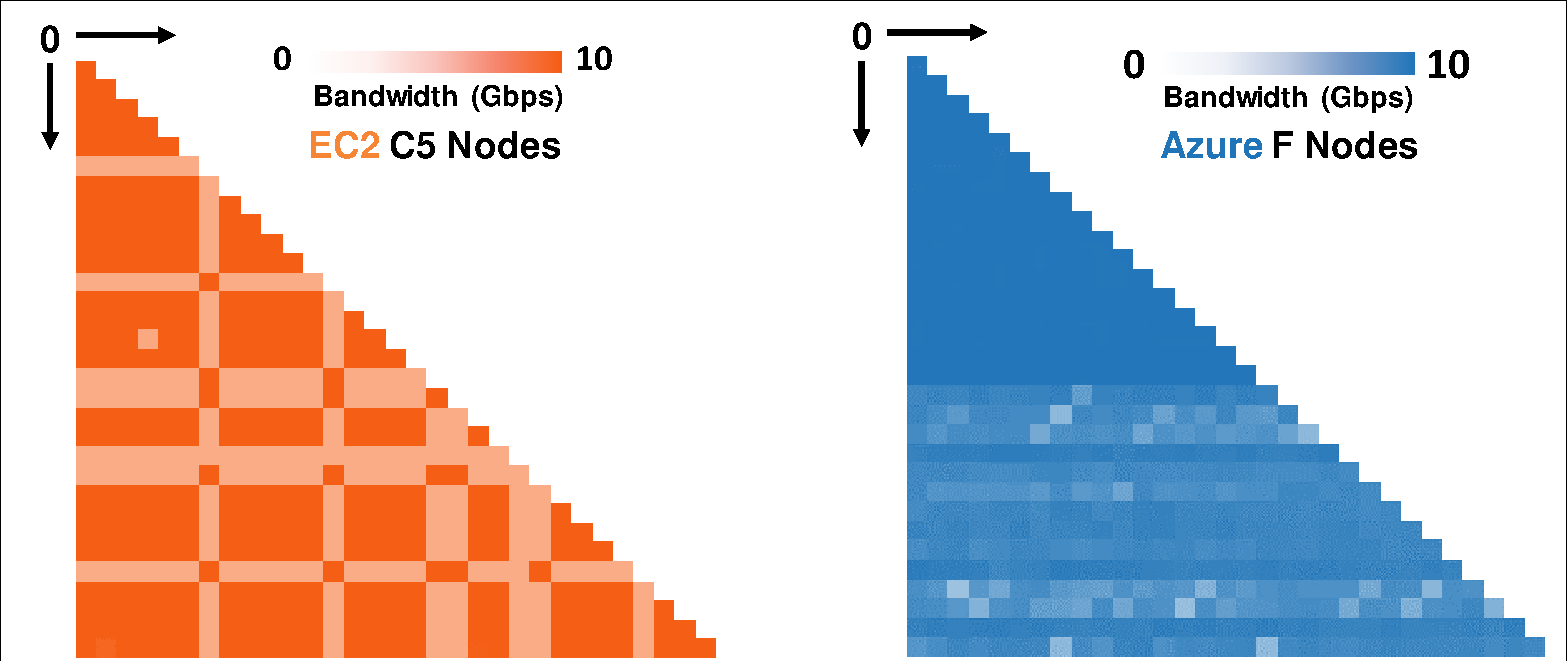
\includegraphics[width=.7\linewidth, trim=3 3 3 3,clip]{Figures/dcnetworkcondition.pdf}
	\caption{Pairwise bandwidth probes with 32 \ectwo C5 and \azure F instances show non-uniform link bandwidth.}
	\label{fig:dcnetworkcondition}
\end{figure}

\begin{figure}[t!]
	\centering
	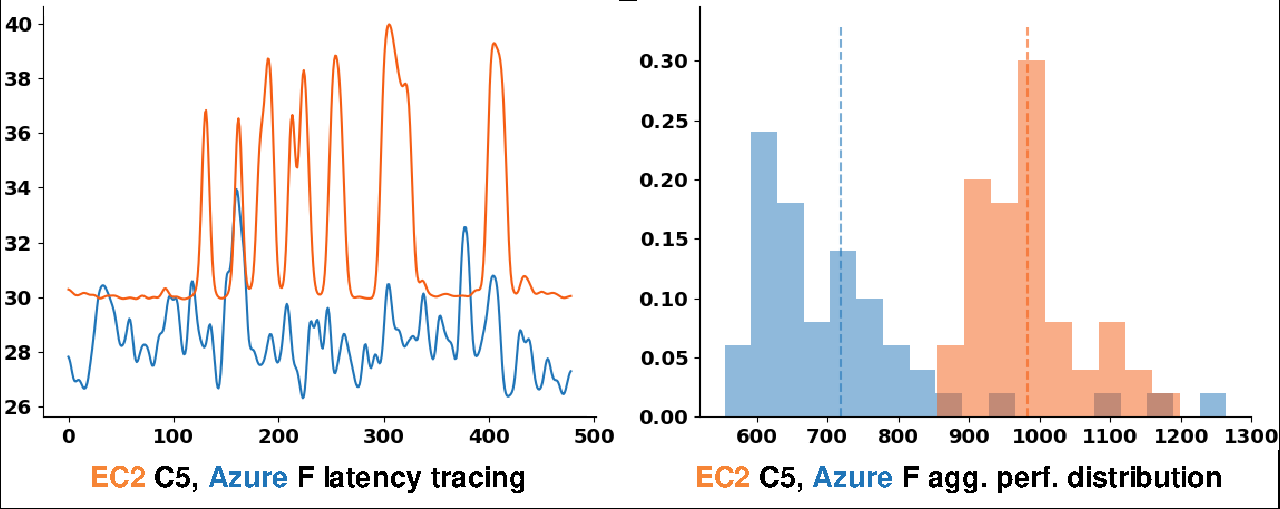
\includegraphics[width=.7\linewidth, trim=3 3 3 3,clip]{Figures/perfFluctuation.pdf}
	\caption{Left: 8 hour latency (us) tracing (1 minute average) between two VMs on both clouds show steep latency fluctuations due to volatile cloud traffic. Right: Wide performance distribution of the same, periodically launched Gloo aggregation task on both clouds.}
	\label{fig:perfFluctuation}
\end{figure}

%\noindent\textbf{One route does not fit all}. The size of model of different layer in a neural network can vary significantly (e.g., the size of the largest layers in the popular ResNet-50 model is multi-megabytes in Caffe2 versus a small layer's model size of hundreds of bytes). This means the transmission time of some layers is latency-bound while some are bandwidth bound. Since the forward and backward passes process layers in a fixed order, a delay in the update of layer L will cause process stall of layer L+1 in forward pass or L-1 in backward pass. Therefore, optimally hiding communication latency requires different aggregation routes for different layers.

\subsubsection{Inefficiencies in Existing Approaches}
\label{sec:differentReductionAlgorithms}
We motivate our design by analyzing why some existing approaches do not perform optimally, as they rely on assumptions that aren't typically valid in the datacenter setting. 

%We first define good locality as localizing communication within a single rack. Thus, the more cross rack communication, the worse locality.

\begin{figure}[t!]
	\centering
	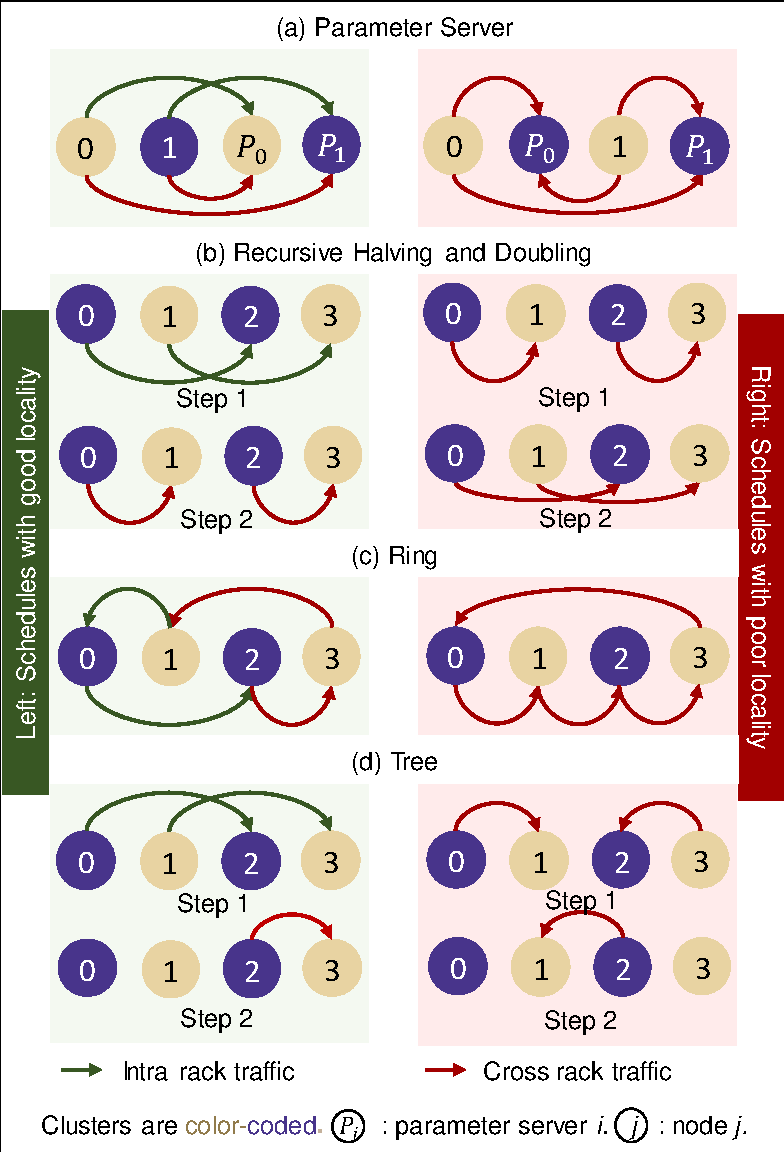
\includegraphics[width=.5\linewidth, trim=3 3 3 3,clip]{Figures/poorlocalitywithexistingapproach.pdf}
	\caption{Existing aggregation approaches can suffer from poor locality if not taking physical network topology into account.} %Some steps omitted for clarity.}
	\label{fig:poorlocalitywithexistingapproach}
\end{figure}

Figure \ref{fig:poorlocalitywithexistingapproach} shows a theoretical analysis of widely used communication patterns. PS (a) and popular choices of CA such as halving-doubling (b) and ring (c) are shown in a setup where nodes (0-3, enclosed in a circle) are spread equally among two clusters (purple and gold).  The left side of the figure shows patterns that achieve optimal locality in the setting by exchanging data among nodes with high locality (high-performance links in green) while minimizing transfers over the bottleneck links (slow links in red). The right side shows alternative reduction routes with poor locality. All patterns achieve the same result, but with different efficiency.

The problem with poor locality happens when the communication pattern in the algorithm is not optimally aligned with physical topology. Mapping logical ranks to physical hosts in a locality-preserving way is contingent on awareness of the physical network structure. Hence, \textit{topology-awareness} is crucial for efficient aggregation in a datacenter network. %For example, in the case of the bad recursive halving-doubling communication highlighted in Figure \ref{fig:poorlocalitywithexistingapproach}(b-right), it would be much better if the IDs of node 1 and 2 are swapped, creating the pattern on the left. %
%Being able to do so 

Even with careful mapping, not all algorithms work optimally in the datacenter environment. Table \ref{table:algoCharacterization} summarizes network characteristics of these algorithms, with a simplified, flattened datacenter network topology model where nodes are simply placed in different racks. Centralized PSs are known to suffer from \textit{incast} congestion and do not scale to a large number of workers~\cite{firecaffe,Geng:2018:HHP:3229543.3229544}. Sharded PSs incur high cross rack traffic. CAs usually trade off lower per-link traffic on the wire with more rounds of communication, which is not suitable when the latency is high. Tree reduction inherits the problems of both PS and CA: high fan-out causes incast problems; a low fan-out adds more rounds. Ultimately, we need an algorithm that bounds communication steps, takes advantage of fast links, and localizes traffic to avoid interference from competing traffic.

\begin{table}[ht]
	\centering
	\begin{tabular}{|c|c|c|c|}
		\hline 
		Name & Rounds/Hops & Bytes on Wire & XR Bytes \\
		\hline
		PS (fully sharded)  & $2$ & $2(NC-1)S$ & $2N(C-1)S$  \\
		\hline
		Halving doubling & $2log_2NC$ & $2NCS$ & $2C\frac{N-1}{N}S$ \\ 
		\hline 
		Ring-Chunked & $2NC-1$ & $(2NC-1)S$ & $(2C-1)S$ \\
		\hline
        Tree (fan out = C) & $2(log_CN + 1)$ & $\approx2C\frac{CN-1}{C-1}S $ & $\approx2C\frac{(N-1)}{C-1}S$ \\ %n is a power of k. each k link starting from the 2nd layer, at least k-1/k links are cross machine link
        \hline
        \hline
        2-level hierarchical & $4$ & $2S(NC-1)$ & $2(C-1)S$ \\
		\hline
	\end{tabular}
	\caption{Network characteristics of various algorithms featuring rounds of communication (Rounds), minimum total traffic (Bytes on Wire), and minimum cross rack traffic (Min XR Bytes, corresponding to red arrows in Figure~\ref{fig:poorlocalitywithexistingapproach}) to allreduce with $NC$ nodes on $C$ racks, each with $N$ nodes. Each node has a buffer of size $S$ bytes. PS and aggregators in HA are colocated and sharded.}
	\label{table:algoCharacterization}
\end{table}

\subsubsection{2-level Hierarchical Aggregation (2LHA)}
HA is not new, but most applications of \mlha are in contexts where the network topology is known. HA does not reduce the total amount of data transferred on the wire, but it can create more \textit{localized} traffic and avoid slow links.

%trades more \textit{localized} traffic with higher \textit{latency}, because a piece of data needs to traverse multiple hops.

%The potential benefit comes from traffic localization, which is related to the tree-like topology: with each hop the message takes, exponentially more machines can generate adversarial traffic that affects this message.
One important parameter in HA is the number of levels. Similar to~\cite{cool}, we used a 2-level HA based on our domain knowledge of datacenter networks, that oversubscription mostly hurts at the rack level. Thus, by separating inter- and intra-rack aggregation, we can best capture the static aspect of locality and minimize latency. The use of more levels ($>2$) suffers from higher latency and volatile performance, as messages need to traverse multiple links with unpredictable latency, but provides no benefit compared to PS if links don't have enough non-uniformity (e.g., in the same cluster). %Therefore, we focus on a 2-level hierarchical (2LHA) aggregation scheme because it strikes a balance between smaller latency (requiring fewer rounds) and more aggressive localization (requiring more rounds).

%, and empirically can capture the network locality well~(\textsection\ref{sec:eval}).

\label{sec:2lhaOverview}
\mlha partitions nodes into different groups (clusters) based on their affinity. \mlha starts by chunking the buffer across members in the same group. For each chunk, a node is designated as the local master (LM) for that group for aggregating locally. One of the LMs across all groups is chosen as the global master (GM) for global aggregation. Visually, the reduction trees of all chunks form a 2-level forest. Communication for \mlha is done in the following steps: 

\begin{enumerate}[noitemsep,topsep=0pt,parsep=0pt,partopsep=0pt]
  \item Each group member sends all chunks to their respective LMs (intra-group traffic only).
  \item LMs in all groups send per-group aggregated chunk to the GM for global aggregation (inter-group traffic only).
  \item The GM aggregates the chunk, then uses the reversed routes for propagating the globally-aggregated chunk back to the LMs.
  \item The LMs fan out the globally aggregated chunk to all group members.
\end{enumerate}

%\arvind{say something about sharding and load balancing of chunks?}

%\begin{figure}
%	\centering
%	\includegraphics[width=.9\linewidth, trim=1 3 3 3,clip]{Figures/2LHA.pdf}
%	\caption{The first two steps in performing a \mlha for chunk 1 labelled. Gradients are aggregated locally before synchronized globally, reducing data transferred on inter-group links.}
%	\label{fig:2lha}
%\end{figure}

\mlha is described here as a two-phase process for simplicity, but the intra- and inter-group aggregation can overlap. Effective \mlha also requires load-balanced LM and GM assignments within and across groups. Later we provide an implementation that satisfies these. Table \ref{table:algoCharacterization} shows the desirable properties of \mlha. Compared to CAs, the number of rounds in \mlha does not increase with the number of nodes and, compared to PSs, it requires significantly less cross-rack bandwidth.

\subsection{Design and Implementation of \plink}

We now describe \plink, an optimized, topology-aware, and dynamic system that leverages HA for efficient cloud-based training. To optimally utilize datacenter networks, \plink must address the major challenges highlighted previously. \plink uses three components to achieve this.
\begin{itemize}[noitemsep,topsep=0pt,parsep=0pt,partopsep=0pt,leftmargin=1em]
    \item \marcopolo: a network probing and clustering approach to capture physical locality in the datacenter network. \marcopolo groups nodes based on their physical affinity, so intra-group links have better communication performance than inter-group links. %\arvind{say "better communication performance" rather than "lower latency"?}
    \item \ha: a high-performance implementation of \mlha that is codesigned to take advantage of deep learning properties. %\arvind{what do you mean by training workload?}
    \ha uses clustering information to  distribute the aggregation workload efficiently and execute the aggregation schedule.
    \item \autoplink: a mechanism that tracks training performance and adjusts the current GM and LM assignments to adapt to changes in the network conditions.
\end{itemize}

\subsubsection{Capturing Network Locality with \marcopolo}
\label{sec:marcopolo}
For accurate network topology discovery, \marcopolo must probe quickly and should not rely on knowledge of a particular datacenter. \marcopolo: (1) probes communication links between nodes to measure pairwise node distances, (2) denoises probed distances, and (3) clusters nodes.

\paragraph{Running \marcopolo probes}

\marcopolo starts by issuing measurements to identify communication locality and determine pairwise node distances. Distance is defined using universal networking concepts, like latency or inverse bandwidth. \marcopolo uses two different probes: an inhouse DPDK-based~\cite{HomeDPDK74:online} probe to provide near bare-metal latency measurements for supported VMs on \azure and \ectwo, and iPerf~\cite{iPerfThe0:online}. \marcopolo runs these networking probes one-to-one. $O(N^2)$ time would be required to probe $N$ nodes if run sequentially. To accelerate this process, \marcopolo picks as many pairs (up to $\frac{N}{2}$) as possible in each round without having a node appear twice, to avoid interference from concurrent tests. This allows \marcopolo to probe in $O(N)$ rounds.

%\noindent\textbf{All-to-all probes} are one-shot tests that all nodes participate in. \marcopolo use these tests to assess distances of nodes in a more dynamic fashion under loaded conditions. %, as all to all probe resembles the communication pattern of distributed training. 

\marcopolo derives pairwise distances with probe results (in case of bandwidth measurements, bandwidth are converted to distance by taking the inverse~\cite{affinity2Distance}). \marcopolo then proceeds to \textit{denoise} the collected data. %, before clustering nodes into different groups based on their physical affinity. %\arvind{be consistent with terminology.  Earlier it is "augment/denoising", now it is "augment", and next it is "refining".  I think "denoising" is better.}

\paragraph{Denoising probe data with embedding}
\label{sec:embedding}
 \marcopolo embeds nodes in a Euclidean coordinate space, obtaining a set of coordinates whose distances agree with the probed distances. This works to:
\begin{enumerate}[noitemsep,topsep=0pt,parsep=0pt,partopsep=0pt]
    \item Denoise measurements by leveraging Euclidean space to approximate the physical location of nodes. %\arvind{I think we can say "which we use to approximate the physical location of nodes inside a datacenter" rather than "resembles a network topology".}
    %Distances in the Euclidean space end up being more reflective of network topology, likely due to denoising effects.
    \item Obtain a set of ``virtual coordinates'' for a clustering algorithm to identify groups.
\end{enumerate}
To embed nodes, we identify node coordinates ($\mathbf{v_i}$ and optional $h_i$) that minimize the following objective:
\begin{equation}
    \sum_{i=1}^n \sum_{j=1}^{i-1} \left( (d_{i,j})^\alpha + \mathbbm{1}_h\left[h_i + h_j \right]  - p_{i,j}\right)^2 
\end{equation}
where $n$ is the number of nodes, $d_{i,j} = \left\lVert \mathbf{v_i} - \mathbf{v_j} \right\rVert_2$ is the Euclidean distance between embedded node coordinates for nodes $i$ and $j$, $p_{i,j}$ is their probed distance, parameter $\alpha$ takes a value between 1 and 2, $h_i$ is a non-negative startup cost parameter for node i, and $\mathbbm{1}_h$ is a switch for $h_i$. We use the Adam algorithm~\cite{kingma2014adam} to optimize this.
%$x$ is a tunable parameter between 1 and 2 that intuitively governs how much emphasis is put on long probed distances in the embedding process. %is an indicator denoting whether or not we are using these latency parameters. % We will describe the use of $h_i$ later in this section, but first consider the case when $\mathbbm{1}_h = 0$.

\marcopolo embeds VM nodes in a coordinate space that preserves the probed distances between VM nodes. The denoising effect of the embedding process stems from its tendency to keep mutually close nodes together, which enforces our domain knowledge that VM nodes that are close to one particular reference VM node are probably close to each other as well in the datacenter. Thus, this effect has a correcting influence when the mutual-closeness property is violated by a particular observation but is observed in a majority of nodes. A lower number of embedding dimensions strengthens this effect.
%Considering only the left size of equation 1 (ignoring $h$), there are 2 cases, one when $x=1$ and one when $x=2$ (the two allowed values). These share a common intuition for why topology might be well captured. In both, we are embedding our nodes in a coordinate space where larger Euclidean distance should correspond to larger probe distance. In such a space, we have the property that, for nodes A, B, and C, if A and B are both close to C by Euclidean distance, they must also be relatively close to each other. This fits our domain knowledge, that if two nodes are close to a mutual third in a datacenter, they should also be relatively close to one another. 
%We have observed noise in the probe distance data that violates this mutual-closeness property, and we believe this is part of why our method is successful. Fitting Euclidean distance enforces this concept of closeness, working to remove that noise, and giving us refined distance with an improved agreement with true topology.

$\alpha$ tunes how longer distances are treated in the Euclidean space: $\alpha=1$ fits the embedded distances to probe distances exactly. For $\alpha>1$, we can achieve increased compaction of distance while maintaining relative distance order. This effect is desired because small physical distances can be magnified disproportionately in the probe due to competing traffic. Setting $\alpha=2$ causes the long probed values to be ``compacted'' more than the smaller ones (but it never changes the relative order of distances). Figure~\ref{fig:legacy_why} suggests empirically, a larger $\alpha$ pushes VM nodes with short distances even closer on the embedded plane, leading to more consistent clusters with higher adjusted mutual information~\cite{vinh2010information} (0.59 vs 0.76) across 100 runs.

% with a larger probe distance being represented by a moderately larger embedding distance, allowing \marcopolo to generate more consistent clusters empirically (higher Adjusted Mutual Information~\cite{vinh2010information} score across many runs).

%It is important to capture long distances as accurately as possible because they are the bottleneck in \mlha. Setting $\alpha > 1$ lets \marcopolo{} focus more on the representation of long distances in the embedding process. Figure~\ref{fig:legacy_why} (right) shows that in the $\alpha=1$ case, the error for deviating from the optimal value of embedding distance ($d$) is independent of probe value $p$, but with $\alpha > 1$, the same deviation for a longer probed distance results in a larger error in the optimization objective, forcing the optimizer to focus on it. %Setting $\alpha > 1$ does exactly this for longer probe distances, which we expect to be more important.


% we're effectively discounting long probe distance in the embedding: only 2X euclidean distance is required to represent a 4X probe distance. Preventing long distances in the embedded space enforces the reality in the datacenter that no distances should be significantly larger than the average distance, so disallowing long distances to be embedded exceedingly far from other nodes in face of a long probed distance (likely due to interference) tends to better capture physical affinity.

%$x$ also controls whether additional focus is given to long distances when minimizing the embedding error: a larger $x$ forces the embedding space to reflect long distances most precisely, which is desirable because \mlha{}'s performance is bottlenecked by the longest distance in each hierarchy. Capturing this is crucial in later generation of the actual clusters. Figure~\ref{fig:legacy_why} gives a visual summary of the effect of $x$: long probed distances are more ''compressed``, and more ''carefully treated`` than short probe distances, resulting in tighter-packed embedded space that resembles datacenter, especially bottlenecks.

Inspired by~\cite{Dabek:2004:VDN:1030194.1015471}, \marcopolo includes an optional parameter $h_i$, the node-specific, network-agnostic, fixed latency of sending a packet (e.g. traversing the operating system network stack). 

Multiple clusters are generated at once, and \marcopolo favors clusters with smaller diversity in the sizes of groups. If there is a tie, \marcopolo makes a random choice.

%\arvind{more comments on the above text: (1) need to state up front what is being solved by the optimization problem; I believe it is both vi as well as hi. (2) $1_h$ seems to be a function of the type of measurement probe that is used (i.e., latency as opposed to bandwidth); if so, say it at the beginning.  (3) even then, it seems like you want to have the hi factors along with the coords (i.e., $v + h - d$) as opposed to being outside. (4) what happens if you have multiple types of measurements?}




%A standard approach to such a problem would just set $x=1$, fitting Euclidean distance to probe distance directly by a sum-of-squares error. In testing a variety of optimization objectives, we found the standard approach ($x=1$) often performed well, but in many cases squaring the Euclidean distance term ($x=2$) gave superior performance. This is the setting we typically use in our experiments on \marcopolo. We will attempt to gives some intuition about why this might be more effective. 

%First, we have useful domain knowledge, that no distances should be significantly larger than the average distance. Nodes are tightly packed in the datacenter, and so we expect their topology to be described by coordinates with no distant outliers. We do however observe such outliers in the data. Using $x=2$ allows nodes with very large probe distances to not be embedded exceedingly far from all other nodes. This is because, for instance, only 2X euclidean distance is required to represent a 4X probe distance.

\begin{figure}
	\centering
	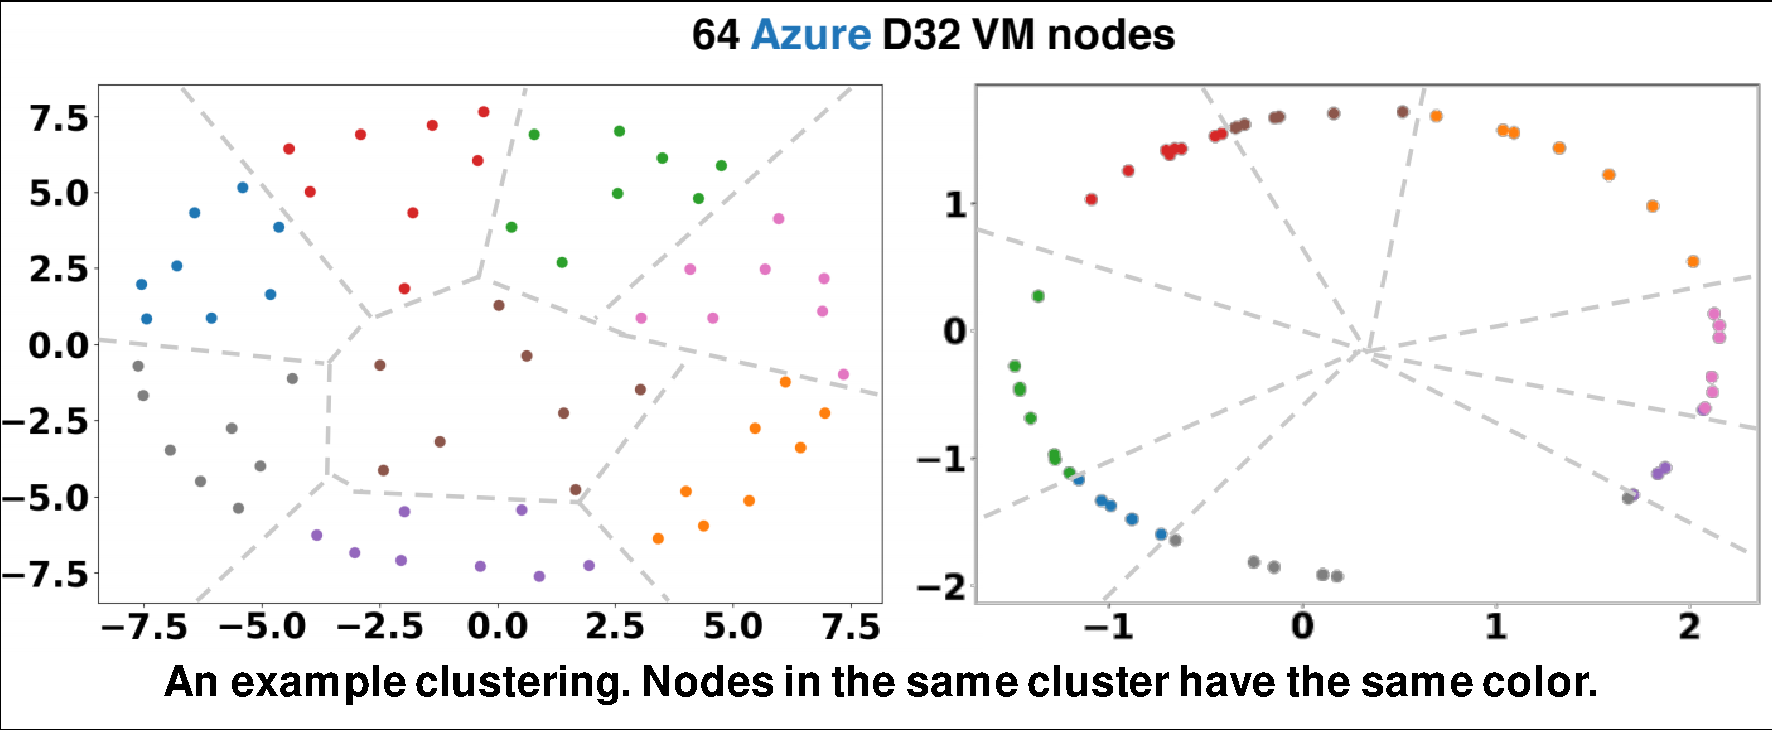
\includegraphics[width=.7\linewidth, trim= 4 4 4 4,clip]{Figures/clusters.pdf}
	\caption{Effect of $\alpha$: $\alpha = 2$ (right) generates more consistent clusters (higher AMI across 100 generated clusters) compared to $\alpha=1$ (left)} % This effectively means the resulting embedding space is more sensitive  long distances than short ones, where it is equally sensitive when $x=1$}
	\label{fig:legacy_why}
\end{figure}


%Second, consider the fact that bottlenecks will likely come from longer distances. For this reason, it can be more important to capture long distances precisely. Figure 4 demonstrates why the $x=2$ case achieves this. If we consider an error margin in capturing probe distance (which is the error we optimize here, by sum-of-squares) we can notice a key difference between $x=1$ and $x=2$. In the $x=1$ case, the error margin in euclidean space required satisfy the probe distance margin does not depend on probe distance. In the $x=2$ case however, a larger probe distance gives us a tighter error margin in Euclidean space, effectively forcing the coordinates to capture larger probe distances more precisely.

%Inspired by the Vivaldi system of \cite{dabek2004vivaldi}, we allow for "height" parameters $h_i$ for each node i. When this feature is enabled ($\mathbbm{1}_h = 1$), $h_i$ corresponds to an added, node-specific distance applied to any distance the node is involved in. We found this useful for improving the system's ability to capture ground-truth topology for some nodes (e.g. ping) but not others, which is why we allow this to be disabled.



\paragraph{Grouping Nodes for \mlha}
We now outline how \marcopolo partitions VM nodes into groups for \mlha. The goal is to generate groups that are (1) balanced, so no single group becomes a bottleneck and (2) cohesive, so VMs in the same group have good locality. We first compute the number of groups to generate, then determine the members of each group.

GMs are more likely to be the bottleneck during \mlha, as they must receive and aggregate messages at both levels. For a uniform key distribution, the following term approximates the bytes-on-wire sent or received by a GM:
\begin{equation}
   b = O\left(\frac{n}{k} + k\right)
\end{equation}
with $n$ total VMs, and $k$ groups. The GM sends and receives a message from each node within its group ($\frac{n}{k} -1$) for local aggregation, and from every other group ($k-1$) for global aggregation. This expression achieves a minimum at $k = \sqrt{n}$, giving a natural choice for group count. %., and it is empirically effective with and without them.

Once group count is selected, we use a constrained k-means clustering algorithm with k-means++ initialization~\cite{bradley2000constrained, arthur2007k} to generate balanced, locality-preserving groups. This accepts a minimum cluster size and the number of groups to generate as input. %\arvind{and number of groups also as input?} 
For perfect balance, both parameters are set to $\sqrt{n}$. %, where $k = \sqrt{n}$ in general. %, we use $k = \sqrt{n}$ (as justified in \strongrandom).

Enforcing perfect balance is not optimal in cases where VMs are naturally clustered in almost balanced but distant clusters, because in those cases some group can contain a distant member which could be assigned to a much more cohesive group with a slight imbalance, forcing an onerous bottleneck on the local aggregation step. Thus, we include a parameter, \textit{balance elasticity}, which enables a slight imbalance among clusters. We empirically found best results with values between 1.0 (perfectly balanced) and 2.0 (each group has at least $\sqrt{N}/2$ nodes). %\arvind{define the parameter -- largest/average or largest/smallest?}

%We include optional parameter $h_i$ from equation 1 which can improve the quality of embedding, but will not affect the clustering objective and can be safely ignored.

In order to evaluate the performance of \marcopolo, we also define \strongrandom, a grouping method for \mlha that operates without considering probe distances and simply produces $\sqrt{n}$ groups of size $\sqrt{n}$ uniformly at random. This is used later as a baseline.

\subsubsection{Efficient HA with \ha}
\label{sec:haimpl}
\ha transforms grouping information from \marcopolo into a hierarchical reduction plan and efficiently executes it. \ha takes the crux of \phub and applies them to a TCP context to accommodate for the cloud environment where InfiniBand is not available.
\ha supports various communication backends, including TCP, RoCE~\cite{softroce}, iWarp~\cite{softiwarp}, and InfiniBand.

%, to maintain compatibility with all environments. We now briefly describe \ha in the context of TCP. %On clouds with Ethernet-only support such as EC2, \ha can still support RDMA with SoftiWarp~\cite{softiwarp} and SoftRoCE~\cite{softroce}, although we didn't find any performance benefit of doing so compared to using a native TCP backend.

\paragraph{Generating an Aggregation Plan}
\label{sec:generatingAggregationPlan}
\ha chunks buffers into 64KB segments for better load-balancing across processor cores and overlapping of the transmission of gradients with aggregation. % but at the cost of potentially more packets. \ha uses chunk size of 64KB. % for TCP and 8KB for RDMA.

%identifying the buffers and their sizes to aggregate. \ha first creates chunks of buffers. Chunks are important if the supplied buffers have various sizes and are hard to balance the load. \ha prefers smaller buffer chunks because they allow for more fine-grained overlapping of data transmission and aggregation, as each chunk can be aggregated independently to take advantage of the fact that aggregation is an element-wise operation. However, a chunk size too small is harmful as they may not saturate the network and requires excessive computation overhead: generally, we find chunk size between the network MTU size (generally 1.5-9KB) and a few hundreds of KBs to be optimal depending on the workload and environment.

%Generally, once \ha has a list of chunks with roughly the same size, it finds each chunk a \textit{local master (LM)} for each clustered group of nodes. LMs take care of leaf-level aggregation of a chunk using central aggregation. \ha then assign one of the LMs as \textit{global master (GM)}, so that LMs only send per-group aggregated chunk to GM, by going through the four steps described in \ref{sec:2lhaOverview}. %Small buffers are treated differently, however: if buffers are small, the time to traverse an additional two hops (with \mlha) may not be compensated by the reduced cross rack traffic. It is better to ignore the cluster topology and treats the network as flat. \ha uses a flat topology for buffer $b$ if $lat(GM(b),LM(b)) \approx \frac{SIZE(b)}{bw(GM(b), LM(b))}$, which means the propagation latency is comparable to transmission delay. Note we use the full bandwidth as an overestimation for this purpose, because in reality the bandwidth is shared by multiple flows. This rule is usually applied to buffers of sizes of tens or hundreds of bytes. 


Since \ha is bottlenecked by the slowest inter-group transfer, which in turn is bottlenecked by the slowest intra-group transfer, \ha assigns chunk GMs and LMs such that each group (or node) has a number of GMs (or LMs) proportional to its cardinality. \ha uses an approximation set partition algorithm to achieve this. %Assignment of LM placements in each group follows a similar fashion. 
%as the aggregate available bandwidth scales with the size of a group. % Now consider the min-cut of the bandwidth for each cross rack link in the inferred cluster. The value of the bandwidth min-cut is proportional to the cardinality of the cluster.%., until it reaches the bandwidth of a physical uplink ($B_{upward}$) from ToR to the network core. % This value is currently a changeable parameter ($B_{upward}$) in \ha. 
%Since aggregation latency is determined by the slowest group, \ha need to balance GM assignments cross racks: more GMs should be placed in larger groups.
%but up to a point. 
 %assign GLMs to different clusters based on the min-cut value. The bandwidth min-cut for each group is estimated as the less of $B_{upward}$ and $|C| * B_{vm}$.


%The same argument goes for RLM placements in each rack. \ha uses a similar mechanism to assign RLMs. This is simpler than assigning GLMs because the min-cut bandwidth of each node is equal to the bandwidth provisioned by the cloud, usually 10Gbps. Since a single TCP connection may not be able to saturate a 10Gbps link (as some cloud limits the bandwidth of a single flow~\cite{Placemen48:online}), during communication, \ha establishes multiple connections to each peer and the total transferred data is load-balanced across all connections.

\ha then generates a schedule that executes the steps in \textsection \ref{sec:2lhaOverview} for each chunk. A schedule consists of a set of chunk-action pairs, where action is one of the following\footnote{With these action primitives, \ha can support arbitrary reduction graphs.}:
\begin{itemize}[noitemsep,topsep=0pt,parsep=0pt,partopsep=0pt]
    \item \textbf{SendTo(nids)}: send the content in the current \textit{merge buffer} to the list of nodes specified in \textit{nids}. SendTo is a non-blocking operation, and its status is inferred by whether subsequently anticipated data is received.
    %\item \textbf{ReceiveFrom(nids)}: receive the content in the merge buffer of \textit{nids}. ReceiveFrom is a blocking operation, and it finishes when all updates are received.
    \item \textbf{ReceiveFrom(nids)}: block until the chunks from \textit{nids} are received and aggregated into the merge buffer.
    \item \textbf{Fetch}: notifies \ha that a framework-supplied buffer is ready to be processed.%a fetch action is taken when the calling framework notifies \ha that a buffer can be read. %Depending on the framework, \ha may create a copy of this buffer in case it is modified during aggregation.
    \item \textbf{Deliver}: writes the content in the merge buffer back to the framework-supplied buffer. %\arvind{Deliver instead of Delivery?}
\end{itemize}

A schedule is represented as a DAG where dependencies are edges and nodes are primitives, avoiding false dependencies between local and global aggregation.

\paragraph{Executing an Aggregation Schedule}
\label{sec:2lhae}

%When a job starts, \ha creates two merge buffers for each chunk (details below) and one receive buffer for each peer. %Merge buffers are padded to the nearest cache-line size for efficient reduction using SSE or AVX. 
\ha first performs rendezvous with an out-of-band mechanism (e.g., Redis), establishing multiple connections per pair of VM as cloud providers can restrict per-stream bandwidth~\cite{Placemen48:online}. \ha preserves intra-node locality by maintaining a load-balanced map from a chunk to a connection, and then by further associating the connection to a particular processor core~\cite{Pesterev:2012:INC:2168836.2168870}.

%\ha then connects the mesh prescribed by the schedule. For TCP connections, \ha maintains two flows per network device per remote node to saturate bandwidth; for RDMA-based backends, \ha maintains one connection per network device per remote node (\ha can always materialize additional virtual interfaces as needed). The rendezvous of addresses (IP ports and QP numbers) and memory regions are performed using a central redis server. 

%\begin{figure}
%	\centering
%	\includegraphics[width=\linewidth, trim=0.5 0 0 3,clip]{Figures/2lhae.pdf}
%	\caption{\ha preserves locality by associating a chunk with a particular core and a connection.} % This effectively means the resulting embedding space is more sensitive  long distances than short ones, where it is equally sensitive when $x=1$}
%	\label{fig:2lhae}
%\end{figure}

 %(Figure~\ref{fig:2lhae}).

%\ha groups connections by underlying network device. Each device is then associated with one poll descriptor. Each poll descriptor is further tied to a particular processor core, promoting locality~\cite{Pesterev:2012:INC:2168836.2168870}. The buffers that need communication are load-balanced across network devices first, then load-balanced again across connections.

%\ha spawns worker threads to execute a routine event loop. The event loop pulls data in/pushes data out from/to connection, and polls data from \textit{ready queue}, and \textit{defer queue}.

We now focus on how \ha efficiently supports the four actions, hiding communication latency and avoiding excessive synchronization.

When a framework calls \code{reduce(chunk)}, \ha retrieves the thread ID, suspends it, and enqueues \code{chunk} to the ready queue. Its worker threads poll the ready queue to retrieve \code{chunk} and transition the buffer into the Fetch state, copying gradients from the supplied address, then set the state of buffer to SendTo. %If multiple buffers are available, \ha prioritizes the buffer that corresponds to the later layers of the neural network, because they are required first during backward propagation. When fetch of a buffer is done, \ha transfers the buffer state to the next step specified by the schedule, SendTo. 

SendTo is an asynchronous operation that simply enqueues data to a send FIFO queue. A cursor is used for each TCP connection if a send operation cannot finish. \ha enforces that the order of bytes on the wire corresponds exactly to the order in which SendTos are issued. This saves metadata overhead as only a 4B integer per flow that encodes the chunk ID is required.
% Avoiding mixed transfers of different chunks for a single network flow lets \ha minimize metadata overhead, as only a 4B integer that encodes the chunk ID is required. %For RDMA connections, we use immediate field of a \code{ibv\_wr} to encode metadata and choose \code{IBV\_WR\_RDMA\_WRITE\_WITH\_IMM}.


SendTo is followed by ReceiveFrom. \ha allows streaming aggregation for each buffer in ReceiveFrom state to a \textit{merge buffer}. A counter is incremented when a chunk is fully received from a peer, and when the counter reaches the target, this step concludes. \ha transitions current buffer state to SendTo or Deliver based on schedule. 
%the \ha worker thread aggregates that chunk to the current merge buffer (aggregation can start at a single floating point granularity, but \ha uses SSE or AVX to aggregate whenever possible). A counter associated with a merge buffer is then incremented. 
%When the counter reaches the expected number, ReceiveFrom for that buffer is finished, and the schedule transitions into the next step, which can be another SendTo, or Delivery.


The last step of a schedule is Deliver, where \ha copies the final value to the framework-supplied address. \ha then wakes up the thread that called \code{reduce}. \ha alternates between two merge buffers per chunk for synchronous training to overlap local computation on a chunk with transfers of that chunk to peer nodes.
%Since \ha cannot immediately reuse the merge buffer from last iteration, as the transfer to peer nodes may not finish. \ha alternates two merge buffers per chunk for synchronous training because the peers lag behind at most one iteration. %The flipping step is required because SendTo is asynchronous and can finish before data is on the wire. 
%If the training framework calls \code{reduce} again, the newly-fetched data will overwrite the original merge buffer. 


%Note that the framework does not call another \code{reduce} with the same \code{bufferID} when one is active. Since it is certain when iteration $i+1$ finishes, all merge buffers for all keys of iteration $i$ would have already been sent out (otherwise if remote peers did not receive buffers for iteration $i$, they would not participate in finishing iteration $i+1$ in the first place!). By taking advantage of training is synchronous, we can use two merge buffers to avoid waiting for a SendTo completion signal.

%Not all nodes proceed at the same speed as slower nodes may see incoming data from faster nodes without having the buffer state in ReceiveFrom. In this case, \ha eagerly accepts the data in the receive buffer, without touching the merge buffer because it may be overwritten by a late \code{reduce} call. \ha bookmarks the incoming chunk ID to a deferred queue, which is polled frequently to check if any progress can be made. 
%Saving data to the receive buffer when not in ReceiveFrom state is safe, because each peer only sends one copy of data for each chunk. 

%because \ha is sure that a buffer is sent exactly once per iteration. For bookkeeping, \ha maintains a deferred queue, which is queried later. 



%\subsubsection{Changing an Aggregation Schedule}
%\label{sec:changingPlan}
%\ha dynamically swaps in new aggregation plans to react to network changes by reassigning LMs and GMs. This can be implemented efficiently as coherence is optional in DL~\cite{recht2011hogwild, Wei:2015:MCC:2806777.2806778,BSP,SSP,Litz,orpheus}.% shows it is not required to achieve high accuracy. %\ha can get away by taking advantage that learning itself is a stochastic process: by maintaining a keeping a strongly coherent view of model during normal operation and a bounded-staled, relaxed view of model during change of aggregation schedule, which is known to not affect accuracy

%Schedule changes start by blocking subsequent calls to \code{reduce}. \ha then attempts to bring its polling threads to a safe point, %so that aggregation schedule for all buffers can be reset to Fetch stage. A safe point is 
%which is reached by first draining the send queue then transitioning the buffer state to Fetch. %, avoiding transferring old data when a new schedule is installed.\
%Each buffer is then given a 5s timeout to do so, and after which \ha signals its peers that it is ready to switch to a new schedule for that chunk. \ha recovers chunks that are affected by requeueing them to the ready queue. 

%\ha supports a transparent process for switching to a new aggregation schedule, with the end result being that chunks whose reductions are interrupted by schedule changes may hold values from the previous iteration, while chunks whose reductions are uninterrupted reflect the new values of the current iteration.

\begin{table}[t]
	\centering
	\small
	%\footnotesize
	\begin{tabular}{|c|c|}
		\hline 
		Property & \ha Optimization \\
		%\hline
		%Wide range of buffer sizes & Size-based agg. route selection. \\
		\hline
		Fixed comm. pattern & No explicit acknowledgement \\
		\hline
		Fixed buffer size & Minimal metadata \\
		%\hline
		%Later layer depended on first & Prioritize later layers \\
		\hline
		One reduction per layer & Only 2 merge buffers per layer; \\
		       per iteration    & Eagerly accepts chunks \\
		\hline
		Training is stochastic & Switching plans quickly and cheaply \\ 
		\hline
		
	\end{tabular}
	\caption{Codesigning \ha with training workload.}
	\label{table:codesign2lha}
\end{table}

Table \ref{table:codesign2lha} summarizes how \ha is designed to take advantage of properties in the distributed training workload to lower its overhead.

\subsubsection{Reacting to Network Changes with \autoplink}
\label{sec:autoplinkimpl}
\autoplink collects performance information from \ha and watches for sudden changes in link conditions, reflected by the current training speed. %Instead of running \marcopolo in the background, which itself is resource intensive, \plink needs to take a lightweight approach that directly pinpoints the link bottleneck of training. 
The goal of \autoplink is to dynamically compensate for link changes by redistributing LMs and GMs to VMs, so the time to finish an iteration is similar at both local and global levels.  %that slower VM nodes are serving less as GM or LM of chunks. %, so that nodes with less bandwidth are assigned fewer chunks. 

A perfect initial LM and GM assignment is hard, even if we have bandwidth probe measurements. Consider an aggregation plan $S$, where the \textit{effective bandwidth} of node $i$ to $j$ while running aggregation $S$ is $BW(i,j)$.  Clearly, finding the best $S$ analytically relies on $BW(i,j)$ to be precisely measured or modeled, but $BW(i,j)$ has a circular dependency on $S$ itself. \autoplink thus makes approximations when optimizing the assignments. %, because it depends on the actual transfers dictated by $S$. %Meanwhile, $BW(i,j)$ might change due to competing traffic. To counteract this effect, the number of bytes transferred from $i$ to $j$ according to $S$, denoted by $D(i,j)$, should also reflect the change. Moreover, the time to compute model updates in different VM nodes may also differ, creating the straggler effect and adding to the complexity. 

%\autoplink cannot simply minimizes each link's individual transfer time, because they all share the bandwidth of a given node, nor can it minimize the maximum transfer time, because $D(i,j)$ constitutes the total transfers for all different stages $p$ in 2LHA, and thus may not overlap with other transfers. 
At a high level, \autoplink works in two phases: (1) a \textit{Quicktune} phase where a one-shot, global adjustment of GM and LM assignments is done to adapt to the network change immediately; and (2) a \textit{Finetune} phase where \autoplink uses a performance model to find the current performance bottleneck in the system, and moves GMs and LMs away from it in a stepwise, increasingly aggressive manner.

\paragraph{Quicktune}
Quicktune aims to minimize the maximum transfer time of each node. Quicktune can be best summarized formally as follows: let $GM(i,c) \in \{0,1\}$ and $LM(i,c) \in \{0,1\}$ be the boolean variables to be solved, which indicate whether node $i$ is the GM or LM of chunk $c$. Let $G(i)$ be the group of node $i$, $|G|$ the number of groups and $S(c)$ the size of $c$ in bytes. Our goal is to:

minimize
\begin{align*}
\small
\label{eq:quicktuneobj}
   \quad max(t_i = \frac{\sum_{c}S(c)(LM(i,c)|G(i)| + GM(i,c)|G|)}{\sum_{n}BW(i,n)})
\end{align*}

subject to
\begin{align*}
\small
    \forall_{i,c} \quad GM(i,c) = 1 \implies LM(i,c) = 1 \\
    \forall_{c} \quad \sum_{i}GM(i, c) = 1 \\
    \forall_{c,g \in G} \quad \sum_{i \in G(g)}LM(i,c) = 1
\end{align*}

Quicktune solves this with an approximation: it first distributes GMs to different groups, with the number of GMs assigned to each group proportional to the group aggregate bandwidth $\sum_{m \in G(i)}\sum_{n \notin G(g)}BW(m,n)$, then distributes LMs inside each group to different members in a similar fashion, using aggregate per node bandwidth.

%This is effective because groups are balanced in \plink \mlha schedules, and there are many more chunks than there are nodes, practically making every node a GM of a certain chunk, so the effect of being a GM in each group can be ignored. 

%To retrieve $BW(i,j)$, \autoplink queries per connection stats directly from the OS~\cite{NetlinkW13:online, mathis2003web100}.% Since this bandwidth is an average reading, \autoplink filters by the \code{app\_limited} field: bandwidth measured only when the outbound throughput is not throttled by the sending application is recorded. To further reduce averaging effects, \autoplink queries this after each successful \code{write} call.

\paragraph{Finetune}
Quicktune is limited as it assumes constant effective bandwidth across different schedules and ignores node balance. Finetune, however, amends this by gradually \textit{evolving the current schedule}, using both the currently measured $D(i,j)$ and $B(i,j)$ to pinpoint the current bottleneck node in the system, and then moves away its load while maintaining balance based on \textit{blame}. Blame for node $i$ ($B(i)$) has two major weighted parts: \textit{time} $t(i)$ and \textit{imbalance} $l(i)$. \autoplink collects per connection stats including link $RTT(i,j)$, bandwidth $BW(i,j)$ through the OS~\cite{NetlinkW13:online, mathis2003web100}, and computes $t(i)=max_{j}RTT(i,j) + \frac{\sum_{j}D(i,j)}{\sum_jBW(i,j)}$ and normalized $\hat{t(i)} = \frac{t(i)}{mean_n t(n)}$. %Note that we use a first order model to predict reduction time, instead of measuring it directly, because actual reduction time includes overheads from other nodes and we shouldn't blame those on node $i$.%
Further, we let $l(i) = \sum_j{D(i,j)}$ and weighted $\hat{l(i)} = \frac{l(i) -  min_nl(n)}{max_nl(n) - min_nl(n)}$. Finally, blame is defined as $\beta \hat{l(i)} + \gamma \hat{t(i)}$.%(empirically, $\beta=1,\gamma=5$).  %Note how $D(i,j)$ is simply read from the previous schedule in Finetune, a core difference to Quicktune.

With blame for each node available, Finetune attempts a move of a single GM (or if not available, an LM) from the node with highest blame to the lowest, if $\frac{max_iB(i)}{min_iB(i)} >\epsilon$ (a configuration parameter). If Finetune repeatedly identifies the same bottleneck node, it moves exponentially more LMs and GMs in each step. %The number to move is reset to 1 if the bottleneck changes.


%Finetune's metrics are directly inspired by those used in profiling concurrent systems, notably~\cite{Anderson:1990:QTT:98460.98518,AUDIT}, which distributes blames to active tasks (root cause) sharing the resource, and focuses on first order effects~\cite{80132,211299} (most blamed nodes first). 

\autoplink uses a central daemon to collect performance metrics and generate new schedules, and is triggered by a sudden change (e.g., larger than 20\%) in training performance. \autoplink signals \ha to install the new schedule. %, which then proceeds with the steps in \textsection\ref{sec:changingPlan}. % to start using the new schedule.

%\arvind{some comments: (1) this overall sounds very heuristicy and will likely make the reviewers complain - the less heuristicy it is, it would be better; (2) not clear we need to describe both quicktune and finetune - might be simpler to just describe finetune; that might help it sound less heuristicy; (3) try to be as precise as possible about the algo.}

\subsubsection{Integration with Training Frameworks}
\label{sec:integration}
Integrating \plink with a training framework is straightforward. \plink{}'s initialization requires only a list of nodes and buffer sizes/addresses from the training framework. %Reduction is done by calling \code{reduce} in appropriate places.
Here we demonstrate how \plink can be integrated with systems with training frameworks that have different design decisions.

Caffe2/Pytorch uses blocking reduction. \plink integration is done by extending Gloo~\cite{facebook35:online}'s \code{algorithm} object. Caffe2/Pytorch, by default, uses a concurrency limit to control the number of established connections per peer and simultaneous \code{allreduce} calls. \plink instead uses a single \ha instance to multiplex all requests.

MxNet uses an asynchronous callback pattern, but \plink{}'s \code{reduce} is blocking. A separate thread is launched for invoking callbacks through \code{kv\_apps}'s infrastructure when a chunk has finished. Support for MxNet is enabled by extending PSLite~\cite{dmlcpsli50:online}'s \code{van} object. %Initialization of \plink is done by hooking into the \code{init} call of \code{kv\_dist\_server}.


\chapter{PLink Collectives: Towards Cloud-aware Collectives with Rank Reordering}
\label{sec:cc}
We now shift our focus from building efficient parameter servers to another popular paradigm: collectives, used in popular training frameworks such as Caffe2 and Pytorch, where there is no longer role of servers and workers. We also address the need for specialization on alternative interconnects other than a fat tree topology in the datacenter, e.g., with a torus ring in Google TPU pods, because in these highly specialized environments, our optimizations highlighted earlier may not be sufficient. 

%Our experimental application of \cmpi on \textit{allreduce} operations in public clouds results in a speedup of up to 3.7x in multiple microbenchmarks and 1.3x in real-world workloads of distributed training of deep neural networks and gradient boosted decision trees using state-of-the-art frameworks.

\section{Unoptimal use of Collectives Today}
Unfortunately, achieving good \mpi performance in a cloud environment is fundamentally more challenging than in an HPC world, because the user has no control over node placement, topology and has to share the infrastructure with other tenants. These constraints have a strong implication on the performance of \mpi. As a result, the bottleneck of running these workloads with \mpi on the cloud has shifted from computation to communication~\cite{7092922}.

%

\begin{figure}[ht]
    \centering
    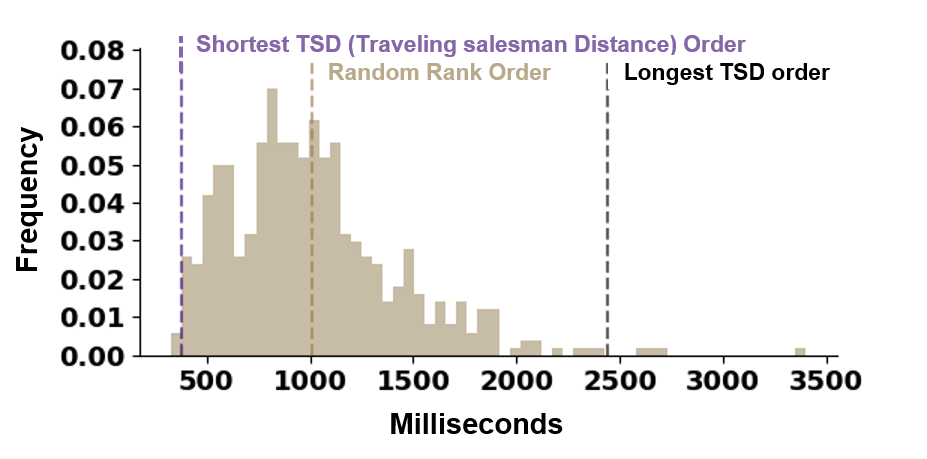
\includegraphics[width=.5\linewidth, trim=8 3 14 10,clip]{Figures/azringperformance.png}
    \caption{Performance distribution of \textit{allreduce} task of 100MB data with ring algorithm varies widely with 500 random rank orders on \azure.}
    \label{fig:azringperformance}
\end{figure}


Consider a common practice of applying \textit{allreduce} ring \mpi, a popular algorithm, in the cloud context, where a randomly-ordered IP list (obtained through the provider) of VMs is used to form a virtual ring on which data is passed along, with $i$-th VM sending data to $i+1$-th VM. But do different ways of forming ring (through permutation of VMs in the list) exhibit the same performance? The answer is most likely no, as the ring that corresponds to shorter total hop cost will likely perform better~(Figure~\ref{fig:azringperformance}). On the other hand, not all ways of forming rings achieve the same cost, because the \textit{point to point communication cost (bandwidth, latency, or collectively referred to as locality in this work) is different across VMs}~(Figure~\ref{fig:dcnetworkcondition}), due to the hierarchical structure of the datacenter network, and the dynamic nature of traffic from other tenants. Consequently, running \mpi with a randomly-ordered list of VMs results in unpredictable and subpar performance. 

Our work focuses on discovering a permutation of the IP list that exploits the network locality for efficient communication, in a completely transparent way, by minimizing the cost model of a given \mpi parameterized with the actual hop cost. To do so, we need to (1) efficiently identify the underlying network bandwidth/latency constraints (or collectively, locality); (2) accurately build cost model for the \mpi at hand; (3) effectively approximate the minimum of these complex cost functions.

This paper proposes \cmpi, a tool that uses accurate network probes to discover locality within the underlying datacenter network, and uses it to solve a communication cost minimization problem with constraints, with the rank of each VM as the unknowns. We use reordered ranks as input to unmodified communication backends in  microbenchmarks including OMB ~\cite{10.1007/978-3-642-33518-1_16}, Nvidia NCCL, Facebook Gloo and
real-world workloads of training deep neural networks with Pytorch/Caffe2 and gradient boosted decision trees using LightGBM~\cite{NIPS2016_6381,Ke2017LightGBMAH} and found a speedup of up to 3.7x in various \textit{allreduce} operations and 1.3x in end-to-end performance across \ectwo and \azure.

\section{Design and Implementation}
\label{sec:designandimpl}
We now describe \cmpi, a tool that takes in a list of VM nodes and a target algorithm, accurately and efficiently probes their pairwise distance, and uses that information to construct a rank order of VMs that attempts to minimize the total cost of communication.

\subsection{Cost Models for Collective Algorithms}
\cmpi builds a cost model $\mathbb{C}_\mathbb{O}$ for each popular algorithm used in \mpi $\mathbb{O}$, parameterized with the number of participating nodes $N$ and size $S$. This section details the cost models for popular algorithms. We use $c_{i,j}(S)$ to refer to the cost for transferring $S$ amount of data from node $i$ to $j$. We further define $MAX_{i=0}^{j}(f(i)) = MAX(f(0),...,f(j))$. We assume $N$ a power of 2 to simplify explanation, and allow arbitrary rank $r$ to alias to canonical rank $(r + N) \text{ mod } N$.
 
\noindent\textbf{Ring}. The cost model of the ring algorithm is the sum of the cost of each hop when traversing the ring: 

$$\mathbb{C}_{r}(N, c, S) = \sum_{i=0}^{N-1} c_{i,i-1}(S)$$

\noindent\textbf{Having Doubling}. The cost of halving doubling is the sum of costs for each round of communication, which in turn is the max cost of all communications in that round. 

$$\mathbb{C}_{hd}(N, c, S) = \sum_{i=0}^{log_2N-1}MAX_{j=0}^{\frac{N}{2}-1}c_{j,j+2^i}(\frac{S}{2^{i+1}}) $$

\noindent\textbf{Tree}. The cost of running tree algorithms depends on the number of trees and how trees are constructed. The total cost is the maximum cost of all trees, which is in turn determined by the maximum cost of each subtree. We provide a cost model for a popular variant of tree algorithm: double binary tree as used in~\cite{nccl}.
$$\mathbb{C}_{dbt}(N, c, S) = T(0,N-1,S)$$
where $T(i,j,S)$ is expressed recursively: 
\begin{align*}
 T(i,j,S) = 
 \left\lbrace
\begin{array}{l@{}l}
0 \textbf{ if $i \ge j$}\\
MAX(c_{\frac{i+j}{2}, \frac{3i+j}{2}-1}(\frac{S}{2}) + T(i, \frac{i+j}{2}-1), \\
c_{\frac{i+j}{2}, \frac{i+3j}{2}+1}(\frac{S}{2}) + T(\frac{i+j}{2}+1, j)) \textbf{ otherwise}
\end{array}
\right.
\end{align*}
Similarly a mirrored tree is built by decrementing each node's rank in the tree without changing the tree structure.

\noindent\textbf{BCube}. The cost of running the BCube algorithm is similar to halving doubling, except in each round, each node communicates with $B-1$ peers, instead of 1.

{\small
$$\mathbb{C}_{b}(N, c, S, B) = \sum_{i=0}^{log_BN-1}MAX_{j=0}^{\frac{N}{B}-1}MAX_{k=1}^{B}c_{j,j+kB^i}(\frac{S}{B^{i+1}}) $$
}

\subsection{Probing for Pairwise Distance}
\label{sec:probinglatency}
We need to determine values for $c_{i,j}(S)$ with end-to-end measurements. We first consider commonly used, simple linear model: $c_{i,j} = LAT_{i,j} + \frac{S}{BW_{i,j,S}}$ where $LAT_{i,j}$ being the one-direction latency from $i$ to $j$, and $BW_{i,j,S}$ the bandwidth achieved with data size of $S$. There are immediate challenges of deriving $BW_{i,j}$ correctly: first, $BW_{i,j,S}$ varies depending on the size of packet size $S$ being transferred: e.g., on a 10Gbps link it is unlikely to saturate full bandwidth while sending small packets. Figure~\ref{fig:tcpchartacteristics} (left) shows the how bandwidth varies with the size of the buffer in a point to point \textit{iperf} (TCP, using DCTCP~\cite{10.1145/1851182.1851192}) test on two 30Gbps D64 nodes on \azure. It is cumbersome to create such profile for each pair of VMs; second, even if a profile like this is constructed, it may still fall short when multiple streams are competing for bandwidth: the streams do not share the bandwidth equally, but rather, one stream can consistently outperform the other in a long time trace, as shown in Figure~\ref{fig:tcpchartacteristics} (right) with 3 D64 nodes on \azure, when both of them can achieve similar throughput when run individually. It seems intractable to derive an accurate $BW$ given $S$ and a set of competing streams. Third, many algorithms operate in chunked mode, allowing overlapping of sending (of processed elements) and receiving (of unprocessed elements), and the simple model does not capture this in the first place. 

It is both beneficial and interesting to accurately model throughput behavior in a multi-stream environment~\cite{data-center-tcp-dctcp,tcphsfairness,10.1007/978-3-540-72606-7_86,ha2008cubic}, but that subject is worthy of its own topic. Instead, we compromise by dropping the bandwidth component in the model, leaving only the latency component. The rationale behind this stems from the well-known theoretical TCP bandwidth model of $BW=O(\frac{MSS}{RTT\sqrt{p}})$ ~\cite{mathis1997macroscopic} given constant drop rate $p$ and window $MSS$. The fact that higher latency induces lower bandwidth in TCP streams lets us approximate costs by only probing for latency.

To accurately and efficiently probe for pairwise latency, we built an in-house DPDK based echo tool, leveraging network enhancement provided by the clouds~\cite{Createan37:online, Enablean80:online}. Probing of $N$ nodes can finish in $N$ rounds, with each round probing for $N/2$ pairs of VMs. At round $r$, node $i$ sends $10k$ probes to $(i + r + 1) \text{ mod } N$ and responds to $10k$ probes from $(i - r - 1 + N) \text{ mod } N$ sequentially. To derive an accurate reading, we take the RTT of 10th percentile. Each probe is a UDP packet with a 32-bit payload that encodes sequence number and round id for fault tolerance. When DPDK cannot be used, we use \textit{fping}, a ICMP Echo-based latency probing tool. For each entry in $c$, we update $c_{i,j} \leftarrow MAX(c_{i,j}, c_{j,i})$ to make it symmetric.


\begin{figure}[t!]
    \centering
    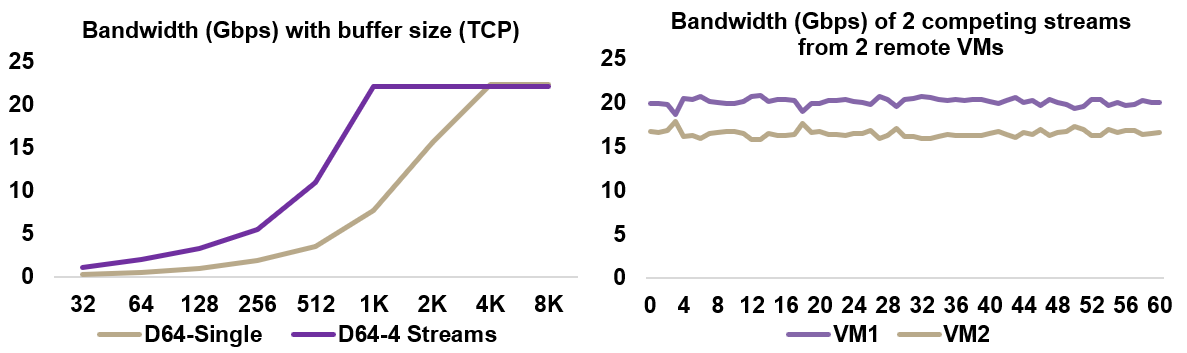
\includegraphics[width=.7\linewidth]{Figures/tcpchartacteristics.png}
    \caption{Left: TCP throughput depends on the buffer size and the number of concurrent streams. Right: while TCP is designed to be fair, an empirical 60s trace in the cloud shows the two streams connecting to the same VM from two other remote VMs do not share the bandwidth equally.}
    \label{fig:tcpchartacteristics}
\end{figure}



\subsection{Minimizing the Cost Model}
We parameterize the cost model with values of probed $c$. To derive a rank ordering that minimizes $\mathbb{C_O}$, we perform the following transformation: let set of variables $\mathbb{R}$ defined as $r_i, i \in [0,N-1]$ be a permutation of $[0,N-1]$ to be solved, and we replace each $c_{i,j}$ with $c_{r_i,r_j}$. We can then establish a bijection from the original rank ordering to the desired order $r_i \leftrightarrow i$ once $r_i$s are solved. We flatten $c_{i,j} \leftrightarrow c'_{iN + j}$ to use theory of arrays to allow direct solving with conventional optimizing SMT solvers such as Z3~\cite{de2008z3,ORToolsG24:online}. 

Unfortunately, we find solvers inefficient, perhaps due to the non-convex, non-linear nature of the objective function and a large search space ($N!$). Instead, we take a two-stage process. The first step employs a range of stochastic search techniques such as simulated annealing~\cite{simanneal}, with a few standard heuristics (e.g., permuting a random sub-array, permuting random pairs) for obtaining neighboring states and a timeout. When the search returns with an initial result $C_0$, we generate an additional SMT constraint $\mathbb{C_O} < C_0$ to better guide pruning for solvers. We let the solver continue to run for a few minutes, and we either find a better solution or will use $C_0$ as the final value. The end-product of this process is a rearranged list of VMs.
\chapter {Evaluation}
We now evaluate the effectiveness of \pbox, \phub and \plink in their perspective environments in accelerating distributed training workloads.

\section{Effectiveness of \phub and \pbox}
We added support for \phub{}'s API to MxNet, replacing its PS. We evaluated \phub by comparing it to MxNet's unmodified PS. We had five goals in our evaluation: (1) to assess the impact of \phub software and the \pbox hardware on training throughput, (2) to identify the importance of each optimization, (3) to determine the limits of \pbox, (4) to evaluate effectiveness of \pbox as a rack-scale service. and (5) to demonstrate the cost-effectiveness of the \phub.


\subsection{Experimental Setup}
We evaluated our system with 8 worker nodes and one specially configured \pbox node. The workers were dual socket Broadwell Xeon E5-2680 v4 systems 
% with 28 cores at 2.4 GHz -- we can omit details as product model implies clockspeed etc to save some space.
and 64 GB of memory using 8 dual-rank DDR-2400 DIMMs. Each worker had a GTX 1080 Ti GPU % with 11 GBs of memory 
and one Mellanox ConnectX-3 InfiniBand card with 56 Gbps bandwidth in the same NUMA domain. The \pbox machine was a dual socket Broadwell Xeon E5-2690 v4 system with 28 cores % running at 2.6 GHz 
and 128 GBs of memory using 8 dual-rank DDR-2400 DIMMs. \pbox had 10 Mellanox ConnectX-3 InfiniBand cards, with 5 connected to each socket. Hyperthreading was disabled. Machines were connected with a Mellanox SX6025 56 Gbps 36-port switch.

The machines ran CentOS 7.3 with CUDA 8 and CuDNN 7 installed. Our modifications to MxNet and its PS (PS-Lite) were based on commit 2ce8b9a of the master branch in the PS-Lite repo. We built MxNet with GCC 4.8 and configured it to use OpenBLAS and enable SSE, the Distributed Key Value Store, the MxNet Profiler, and OpenMP. We used Jemalloc, as suggested by MxNet.

\subsection{DNNs Used in the Evaluation}
We evaluated \phub{}'s performance by training state-of-the-art deep neural networks using reference code provided with MxNet. %While we did not modify the code, 
%We adjusted layer count, per worker batch size, and the number of workers and servers to launch. 
We implemented a cache-enabled optimizer using SGD with Nesterov's accelerated gradient method \cite{nesterov1983method} and a cache-enabled aggregator for \phub{}. We chose a per GPU batch size of 32 when possible; for ResNet 269 and ResNext 269, we used 16 and 8, respectively, since 32 did not fit in the GPU. We did not use MXNet's GPU memory optimizations~\cite{chen2016training} because they slow down training.

\begin{table}[t!]
	\centering
	\begin{tabular}{|c|c|c|c|}
		\hline 
		Name (Abbr)           & Model Size & Time/batch & Batch \\
		\hline
		AlexNet (AN)      & 194MB & 16ms &  32 \\
		\hline 
		VGG 11 (V11)       & 505MB & 121ms & 32 \\
		\hline
		VGG 19 (V19)      & 548MB & 268ms & 32 \\
		\hline
		GoogleNet (GN)   &  38MB & 100ms & 32 \\
		\hline
		Inception V3 (I3) & 91MB  & 225ms & 32 \\
		\hline
		ResNet 18 (RN18)   & 45MB & 54ms & 32 \\
		\hline
		ResNet 50 (RN50)   & 97MB & 161ms & 32 \\
		\hline  
		ResNet 269 (RN269)  & 390MB & 350ms & 16 \\
		\hline
		ResNext 269 (RX269) & 390MB & 386ms & 8 \\
		\hline
	\end{tabular}
	\caption{Neural networks used in our evaluation. Time/batch refers to the forward and backward compute times for a batch.}
	\label{table:networkCharacterization}
\end{table}


Table \ref{table:networkCharacterization} summarizes the neural networks used in our evaluation, which include both winners of the ImageNet challenge and other recent, popular networks. We used the reported model size from MxNet and measured the forward and backward passes time on a single GPU. % with the batch sizes described previously. %We turned off aggregation and optimization for this measurement; therefore, the time represents only that for forward and backward passes.

We report only training throughput in our evaluation since our modifications did not change accuracy: they did not change the computations that were performed. We trained multiple DNNs to convergence to verify this.



\subsection{Training Performance Evaluation}
%We explored training performance using \phub, normalized to unmodified MxNet's performance. 
We include multiple results to highlight the effects of different software and hardware optimizations on \phub{}'s training performance. We measured training performance by comparing the total time of 200 iterations. We used two IB network configurations. This lets us compare training performance for two different compute/bandwidth ratios: (1) where GPUs were much faster than the network, and (2) with ample network bandwidth resources. In both setups, we used 8 workers.
%Both results reflect the benefit of an optimized gradient processing pipeline from the \phub software stack and the benefit of using hardware with balanced resources (\pbox). %\TODO{DO WE NEED 56Gbps IT LOOKS BAD WITH NEW BASELINE.}

\begin{figure}[t!]
    \centering
	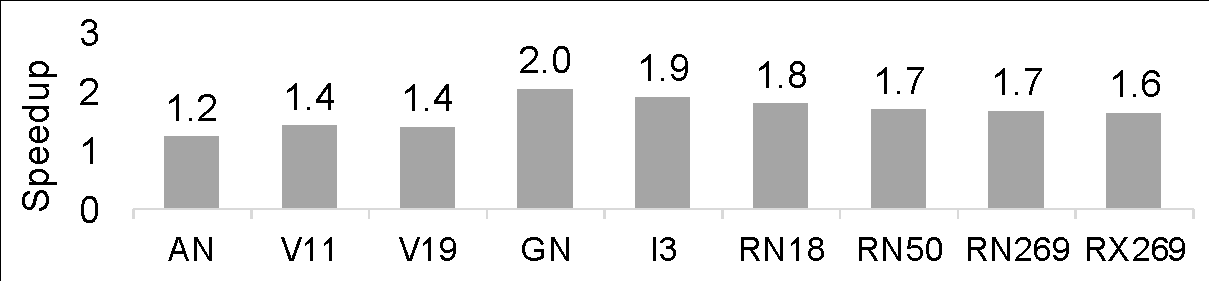
\includegraphics[width=.7\linewidth,trim=8 4 4 4,clip]{Figures/IBBenefits.pdf}
	\caption{Speedup from a faster data plane that supports zero copy.}
	\label{fig:IBBenefits}
\end{figure}

\subsubsection{Benefit of a Faster Data Plane}
Figure \ref{fig:IBBenefits} shows the performance of replacing the communication stack of the MxNet PS with a native InfiniBand implementation (MxNet) that had all optimizations enabled. This lets us see the benefit of switching to an optimized network stack without changing the PS architecture. %We believe similar speedup can be observed on a RoCE-based implementation, because the benefit comes mainly from zero copy. 
We used our \textit{enhanced baseline MxNet} in all the following evaluation.

\subsubsection{Other Software and Hardware Optimizations}
We now quantify further benefits from \phub{}'s software and hardware optimizations. 
We used CS MxNet in this comparison.
\pshard{} results were obtained by running \phub software on each worker as CS PSs. \pbox results represent running \phub software on our single \pbox machine as a NCC PS. We omit results for NCS and CC PSs for clarity. They performed similarly to \pbox results.




% placed here to be on same page as text
\begin{figure*}[t!]
	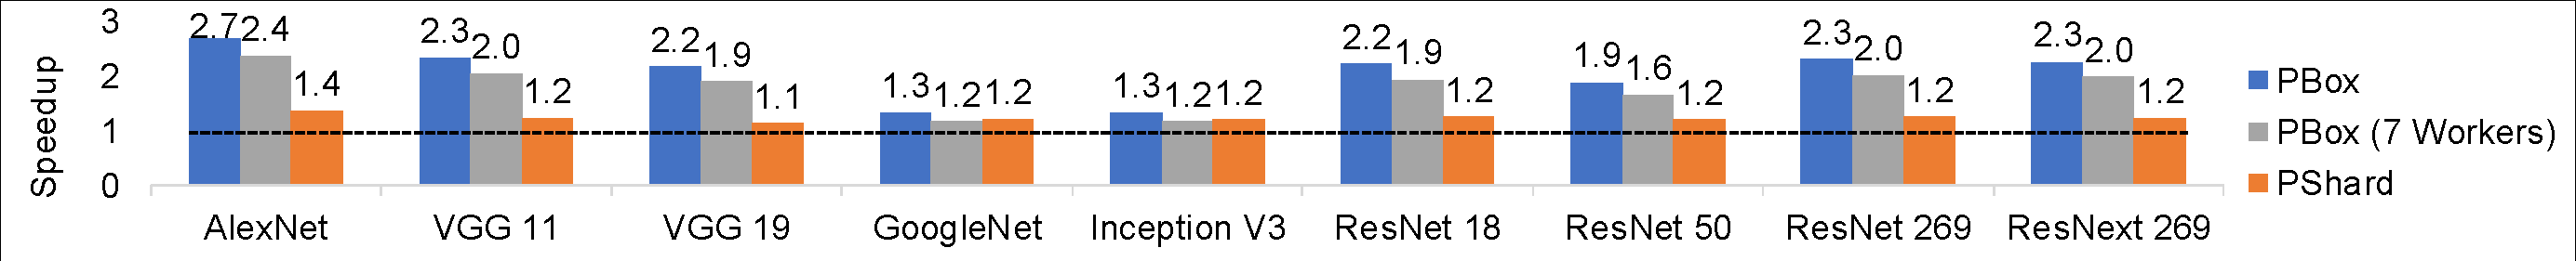
\includegraphics[width=\linewidth,trim=4 4 4 4,clip]{Figures/8GbpsRealTraining_SOCC.pdf}
	\caption{Training performance on a cloud-like 10 Gbps network. Results are normalized to sharded MxNet (\textit{enhanced baseline}).}
	\label{fig:real-8gb}
\end{figure*}

% placed here to be on same page as text
\begin{figure}[t!]
    \centering
	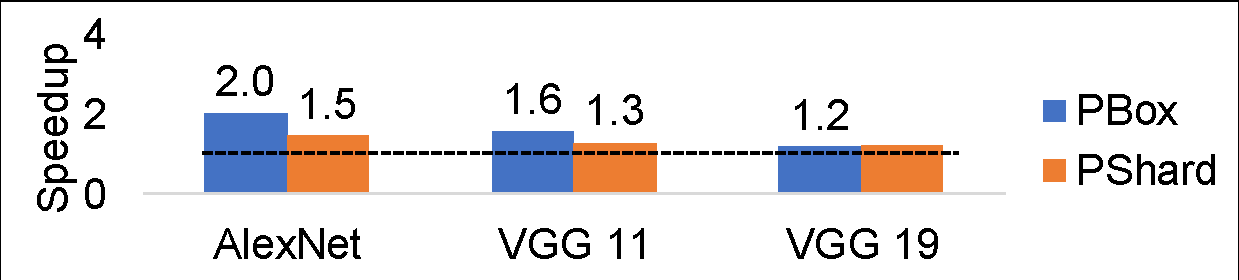
\includegraphics[width=.5\linewidth,trim=8 4 4 4,clip]{Figures/56GbpsRealTraining_SOCC.pdf}
	\caption{Training performance on a 56 Gbps network compared to MxNet (\textit{enhanced baseline}). Computation speed bottlenecked training throughput for all but AlexNet and VGG.}
	\label{fig:real-56gb}
\end{figure}

\begin{figure}
    \centering
	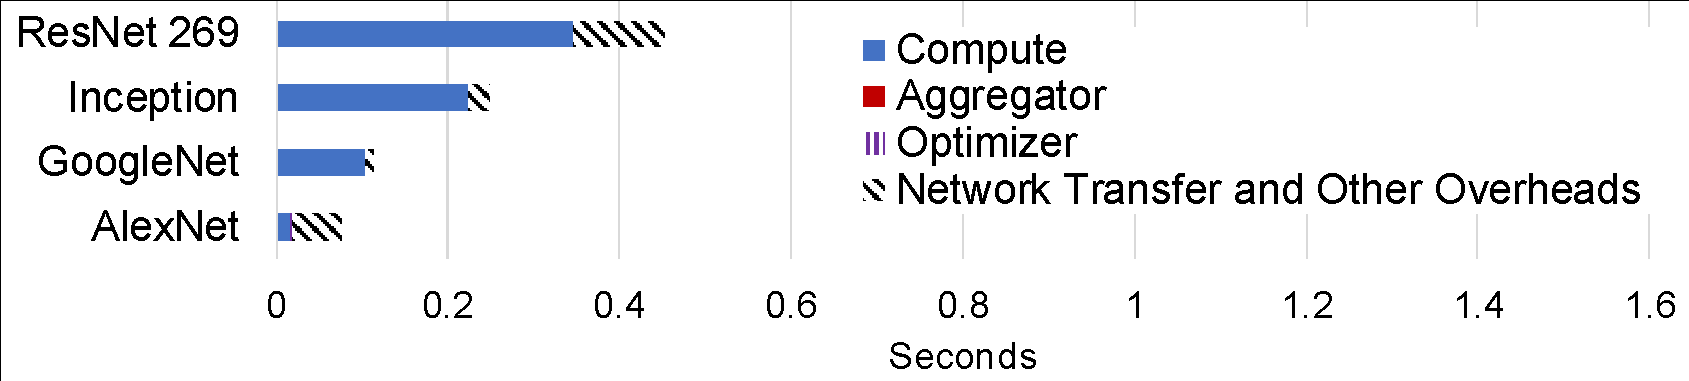
\includegraphics[width=.7\linewidth,trim=4 2 2 4,clip]{Figures/PHubOverheadBreakdown.pdf}
	\caption{Progressive overhead breakdown of \phub. Compared to Figure~\ref{fig:overheadBreakdown}, GPU compute time now dominates training time. Aggregator and optimizer have minimum overhead, and are barely visible.}
	\label{fig:phubOverheadBreakdown}
\end{figure}

Figure~\ref{fig:real-8gb} shows training performance on a cloud-like 10 Gbps network, obtained by down-clocking our IB links. In this configuration, the ratio of GPU batch execution time to network serialization delays is such that the reduced communication and faster aggregation of \pbox significantly affects runtime. In addition, we provide speedup when training with only 7 workers and \pbox, \textit{so that the total machine count in the system is equal to the baseline}.

Figure~\ref{fig:real-56gb} shows training performance on 56 Gbps InfiniBand.
%% In this setup, training throughput of networks such as GoogleNet, Inception, ResNet, and ResNext is limited by speed of forward and backward passes, the time to execute forward and backward passes exceeds that of parameter exchange; thus, raising network bandwidth only marginally affects the total throughput of \phub versus MxNet.
In this setup, for networks such as GoogleNet, Inception, ResNet, and ResNext, forward and backward pass execution time limits training throughput; thus, raising network bandwidth only marginally affects the total throughput of \pbox versus MxNet. Since \phub never slows down training, we omit results of these networks (1x speedup) for clarity. We expect larger speedups with newer, faster GPUs such as the NVidia V100, for these networks. Significant speedup is still achieved with models that have large communication-to-computation ratios, such as AlexNet and VGG; these models remained network-bound even on 56 Gbps links.

%In both cases, the gap between \pbox and \pshard highlights the benefits of non-colocated servers: \textit{they roughly halve the per link bandwidth usage, which makes a significant performance difference in the cloud}. 
The gap between \pshard and MxNet signifies the benefit of software optimizations. The gap between \pshard and \pbox highlights both the benefit of a non-colocated server that \textit{halves the per link bandwidth usage, yielding a significant performance difference}, and the benefit of the hardware optimizations.

%The gap between \pshard and MxNet shows the benefit of \phub software stack optimizations (\mysection\ref{sec:commonOptimizations}), and the gap between MxNet and the baseline reflects the effectiveness of an optimized communication stack (\mysection\ref{sec:IBOptimization}). %\TODO{more explanation}

%Figure~\ref{fig:real-2gb} shows an unbalanced condition where the provisioned compute resource is significantly faster than network bandwidth. We achieved this by reducing our network bandwidth to 2 Gbps; this lets us model the performance of 28x faster GPUs with our 56 Gbps network. Although the baseline parameter servers are more than capable of processing messages at this network speed, the workers' network bandwidth is highly contended by its colocated parameter server instance during parameter synchronization. \phub achieves up to 3x speedup over sharded PSLite-ZMQ by avoiding this worker/shard contention, and providing faster aggregation and optimization.

Figure \ref{fig:phubOverheadBreakdown} breaks down the overhead in different distributed training stages when running \phub in the same setup as Figure \ref{fig:overheadBreakdown}. Compared to Figure \ref{fig:overheadBreakdown}, \textit{\phub reduces overheads from data copy, aggregation, optimization, and synchronization, and fully overlaps these stages, shifting the training back to a compute-bound workload.}


\subsection{Performance with Infinitely Fast Compute}
We used a benchmark to assess the efficiency of \phub{}'s gradient processing pipeline to avoid being bottlenecked by our workers' GPUs. We implemented a special MxNet engine, called \code{ZeroComputeEngine}, based on the original \code{ThreadedEnginePerDevice}, which replaces training operators (such as convolution) with an empty routine. Only the synchronization operators (\code{WaitForVar}, \code{KVStoreDistPush} and \code{KVStoreDistPull}) are actually executed. This engine effectively simulates arbitrarily fast forward and backward passes on the worker side, pushing the limits of \phub.

We used ResNet 18 as the test network. We measured how fast each worker can run in this setup individually with the \pbox, then gradually added more workers to plot total system throughput.

%By spreading the communication equally on the 10 interfaces on the \pbox and utilizing all processors, a worker can perform 110 iterations per second, producing 10GB/s of bidirectional throughput. A single \phub core is enough to saturate a worker. Aggregation and optimization are disabled for this benchmark. We set our "training batch size" to 1 for this benchmark so we measure only the parameter exchange rate. 

Figure \ref{fig:FakeTrainingWithAggOpt} shows the results of running the benchmark with \pbox, \pshard and multiple baseline configurations. \pbox  provided linear scaling with 8 workers and outperformed the baseline by a large margin (up to 40x). \pbox had 2x the speedup of \pshard{} because each of its interfaces needed to move only about half the amount of data compared to colocated servers.

\begin{figure}[t!]
    \centering
	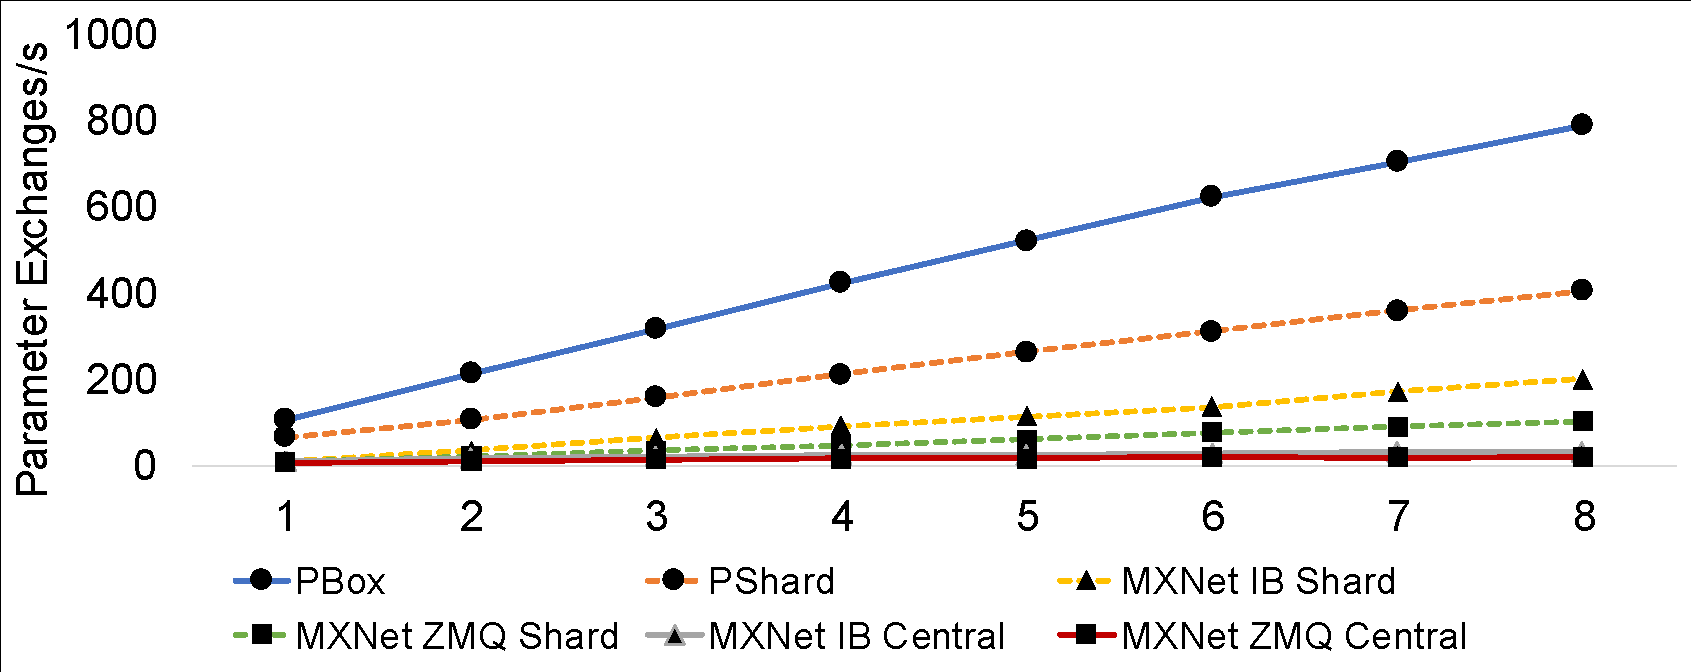
\includegraphics[width=.7\linewidth,trim=3 1 1 3,clip]{Figures/FakeTrainingWithAggOpt.pdf}
	\caption{\pbox provides linear scaling of throughput for 8 worker nodes with infinitely fast compute, training ResNet 18.}
	\label{fig:FakeTrainingWithAggOpt}
\end{figure}


\subsection{Exploiting Locality}
\label{sec:locality}
To postpone hitting the memory bandwidth limit, it is crucial to exploit locality in network interfaces and processor caches. This section evaluates the effectiveness of \phub{}'s key assignment scheme and tall aggregation/optimization in leveraging locality.

\vspace{0.05in}
\noindent \textbf{Key Affinity in \pbox:}
%\subsubsection{Key affinity in \pbox}
\label{sec:affinity}
We evaluate two schemes for connecting workers to \pbox to exploit locality and load balancing. In \textit{Key by Interface/Core mode}, workers partition their keys equally across different interfaces on the \pbox. This mode better utilizes cache by binding a key to a particular interface, core and a NUMA node. %, computation for that key can more effectively use cache. 
This mode also exploits locality in time as workers are likely to generate the same key close to each other in synchronous training.

In \textit{Worker by Interface mode}, each worker communicates with the server through a single interface. This lets \phub exploit locality within a single worker. It also provides naturally perfect load balancing across interfaces and cores at the cost of additional communication and synchronization for each key within the server because keys are scattered across all interfaces and sockets.

%We used the same \code{ZeroComputeEngine} to evaluate the aforementioned approaches. 
We found that Key by Interface/Core provided 1.43x (790 vs 552 exchanges/s) better performance than Worker by Interface mode with \code{ZeroComputeEngine}. The locality within each worker could not compensate for synchronization and memory movement costs.


\vspace{0.05in}
\noindent \textbf{Tall vs. Wide Parallelism:}
%\subsubsection{Tall vs. Wide Aggregation and Optimization}
%Figure \ref{fig:tallVSWide} compares throughput of \phub's tall approach to aggregation and optimization with MxNet's wide approach. 
We evaluated tall aggregation vs MxNet{}'s wide approach with ResNet 50. Tall outperformed wide by 20x in terms of performance  and provides near-perfect scaling to multiple cores. Tall aggregation benefited from increased overlap compared to wide, and wide was further hurt by the cost of synchronization.

%\begin{figure}[t!]
%	\includegraphics[width=\linewidth,trim=3 1 2 3,clip]{Figures/TallVSWide.pdf}
%	\caption{Tall aggregation/optimization was more efficient than wide aggregation/optimization.}
%	\label{fig:tallVSWide}
%\end{figure}

\vspace{0.05in}
\noindent \textbf{Caching Effectiveness in \phub:}
%\subsubsection{Caching effectiveness in \phub}
\label{eval:cache}
Caching benefits many \phub operations. For example, models can be sent directly from cache after being updated, and aggregation buffers can reside in cache near the cores doing aggregation for those keys. We now evaluate the effectiveness of caching in \phub by measuring memory bandwidth usage.

\begin{table}[t!]
	\centering
	\begin{tabular}{|c|c|c|}
		\hline 
		& Mem BW & Throughput\\
		\hline
		Opt/Agg Off & 77.5 & 72.08 \\
		\hline 
		Caching Opt/Agg & 83.5 & 71.6 \\
		\hline
		Cache-bypassed Opt/Agg & 119.7 & 40.48 \\
		\hline
	\end{tabular}
	\caption{Bidirectional memory bandwidth (GB/s) utilization in \phub when training VGG with 8 workers. The maximum memory bandwidth for the machine is 137 GB/s for read-only workloads and 120 GB/s for 1:1 read:write workloads as measured by LikWid and Intel MLC.}
	\label{table:cacheUtilizationAndAggregationOverhead}
\end{table}

Table \ref{table:cacheUtilizationAndAggregationOverhead} shows the memory bandwidth costs of communication, aggregation, and optimization on \pbox. We used 8 workers running a communication-only benchmark based on the VGG network, chosen because it had the largest model size. We first ran the benchmark with no aggregation or optimization, and we then added our two aggregation and optimization implementations.

Without aggregation and optimization, \pbox{}'s bidirectional memory bandwidth usage was stable at 77.5 GB/s. No cache was used in this case because \pbox did not touch the data (only the network interface did).

We found that the caching version of the aggregator and optimizer performed significantly better than the cache-bypassing version, which hit the maximum memory bandwidth available on the \phub machine when combined with the memory bandwidth of worker sends and receives. The caching version, on the other hand, added only 8\% to total memory bandwidth usage; aggregation and optimization added only 1\% of overhead to the overall throughput in this benchmark, fully overlapping gradient transfer. 

\begin{figure}[t!]
	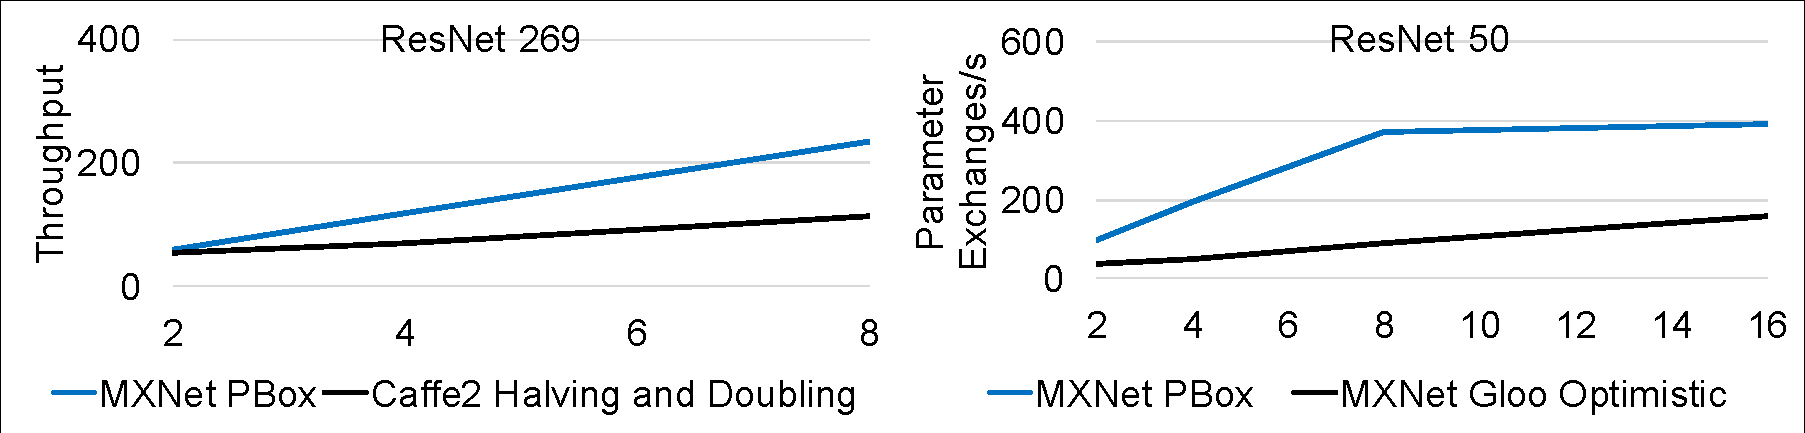
\includegraphics[width=.7\linewidth,trim=8 4 4 4,clip]{Figures/VSGloo.pdf}
	\caption{Left: Comparing Caffe2 + Gloo and MxNet + \pbox on an 10Gbps InfiniBand network. Right: Comparing MxNet + Gloo and MxNet + \pbox on a 56Gbps InfiniBand network with \code{ZeroComputeEngine}. }
	\label{fig:gloo}
\end{figure}

\vspace{0.05in}
\subsection{Comparison with Other Schemes}
%\subsection{Other Communication Schemes}
Parameter servers are not the only way to perform model updates. Frameworks such as CNTK and Caffe2 can use HPC-like approaches, such as collective communication operations~\cite{Thakur:2005:OCC:2747766.2747771, firecaffe}.

To understand how \phub compares to other communication schemes, we first ran Caffe2 and MxNet with \pbox. We used InfiniBand for both systems. We evaluated the fastest algorithm in Gloo: recursive halving and doubling, used in \cite{ImageNetIn1Hour}. Figure \ref{fig:gloo} (left) shows \pbox was nearly 2x faster. 
%This is expected because collectives, like colocated servers, cause roughly 2x traffic per link in the system, bottlenecking training performance in network bound environment.

We ported Gloo to MxNet to better assess both systems. Gloo implements blocking collective operations, but MxNet expects non-blocking operations. Therefore, we measured an optimistic upper bound by letting Gloo start aggregating the entire model as soon as the backward pass started, as if all gradients were available instantaneously. Since Gloo only does reduction, we ran our SGD/Nesterov optimizer on all nodes after reduction was complete. We used 56 Gbps IB and \code{ZeroComputeEngine} to compute bottlenecks. Figure \ref{fig:gloo} (right) shows %when given an infinitely fast compute engine and ample communication resources, 
\pbox sustained higher throughput and provided better scaling up to its limit. Two reasons account for this difference. First, collectives suffer from the same problem as colocated PSs: the interface on each participating node must process nearly 2x the data (Gloo's \code{allreduce} starts with a \code{reduce-scatter} followed by an \code{allgather}~\cite{Thakur:2005:OCC:2747766.2747771}). 
% illustrates the complexity of the scheme). 
Second, collectives frequently use multi-round communication schemes %uses multiple rounds of communication to perform reduction: 
%($logN$ rounds for $N$ workers in this case), 
whereas \pbox uses only 1 round. %, minimizing reduction latency.

% third,  \pbox moves the minimum amount of data in the network: $2MN$, where $M$ is the model size, and halving and doubling moves 

%One interesting point here is that only a fraction of the cores are required to saturate the memory bandwidth when doing aggregation and optimization. Our experiments showed that 4 cores per socket are sufficient to saturate bandwidth for these processors, but to avoid synchronization overhead in the network layer we use one core per interface (5 per socket; 10 total) for the rest of our evaluation.

%We now compare \phub's aggregator and optimizer performance with our baselines using a synthetic benchmark no-computation benchmark based on ResNet-18. Here, we add an additional baseline using MXNet with an allreduce implementation from the Gloo~\cite{Gloo,ImageNetIn1Hour} collectives library. 

%Gloo implements blocking collective operations, but MxNet expects non-blocking operations, so we provide an optimistic upper bound on aggregation performance with Gloo by allowing it to start aggregating the entire model as soon as the backward pass starts, as if the entire gradient is available instantaneously. We evaluate the two fastest algorithms in Gloo: recursive halving and doubling, which is used in \cite{ImageNetIn1Hour}, and chunked ring, which has low analytical complexity and is empirically fast in our measurement. Since Gloo only does reduction, we run our SGD/Nesterov optimizer on all nodes after reduction is complete. We include only a colocated configurations for the sharded baselines in this experiment.

%Figure \ref{fig:cacheUtilizationAndAggregationOverhead} shows the result. \phub beats sharded PSLite-ZMQ and PSLite-IB 7.6x and 3.9x, respectively,  demonstrating the efficient implementation aggregation and optimization in \phub.  \phub also beats Gloo's chunked ring and halving and doubling algorithms by 4.7x and 6.3x, respectively. This is expected since the \phub uses a single round of communication per key, per iteration, whereas for our 8 workers the collective algorithms use 7 and 3 rounds, respectively, and bandwidth is not a bottleneck in this test. We repeated this under a bandwidth limited environment (2Gbps), and found our speedup over these two collectives algorithms is 1.9x and 2.9x. In~\cite{ImageNetIn1Hour}, the halving and doubling algorithm was faster than the chunked ring, but we see the opposite result; we believe this is due to the higher implementation complexity of halving and doubling, and the lower number of workers in our cluster---too few to see the asymptotic complexity benefit. 

%Finally, \phub has a 2x advantage over PShard, which again is limited by network bandwidth due to colocation.


\subsection{Tradeoffs in Fine-Grained Key Chunking}
\label{sec:commParam}
We now examine tradeoffs in the communication layer concerning the size of key chunks and queue pair counts.

\begin{figure}[t!]
    \centering
	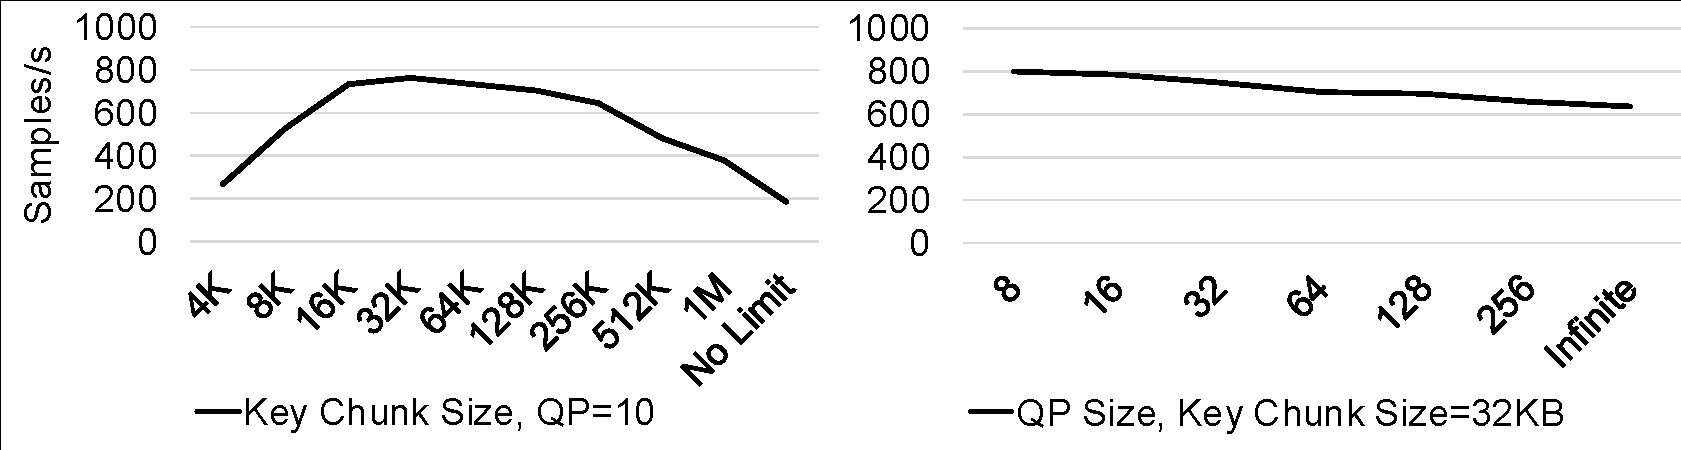
\includegraphics[width=.7\columnwidth,trim=4 8 2 4,clip,]{Figures/QPandKeyChunkSize.pdf}
	\caption{Effect of chunk size and queue pair count on throughput.}
	\label{fig:QPandKeyChunk}
\end{figure}

\vspace{0.05in}
\noindent \textbf{Size of key chunks:}
%\subsubsection{Size of key chunks}
\label{sec:keyChunking}
\phub leverages fine-grained key chunking to better balance load and overlap gradient reception and aggregation. Figure \ref{fig:QPandKeyChunk} (left) evaluates the effect of chunk size with \code{ZeroComputeEngine} on \pbox. Larger chunk sizes improved network utilization, while smaller sizes improved overlapping. We found 32KB chunk size to be optimum: this is likely due to our interfaces' maximum injection rate and aggregation pipeline latency.

\vspace{0.05in}
\noindent \textbf{Queue Pair Count:}
%\subsubsection{Queue Pair Count}
%\phub uses queue pairs to direct keys to cores. The card manages queue pairs; hence, 
A worker needs at least one queue pair per interface with which it communicates. Queue pairs have state, which is cached on the card. When that cache misses frequently, communication slows. For \pbox to use 10 interfaces, we need a minimum of 10 queue pairs per worker. More queue pairs could enable concurrent transmission from the same worker and reduce head of line blocking, but it increases the queue pair cache miss rate. Figure \ref{fig:QPandKeyChunk} (right) evaluates the tradeoff, showing that fewer queue pairs was optimal.





\subsection{Limits on Scalability}
\label{sec:scability} 
The scalability of \phub is inherently limited by available total memory, network or PCIe bandwidth. This section explores how close \phub gets to these limits. We use \pbox to answer these questions. \pbox achieves a 1:1 read:write memory bandwidth of 120 GB/s and a bidirectional network bandwidth of 140 GB/s. To determine how much bandwidth can be utilized,
%we configured varying numbers of worker machines running \code{ib\_write\_bw},
we added an additional IB interface to each of our 8 machines to emulate 16 workers and configured varying numbers of emulated workers running \code{ib\_write\_bw},
%, and configured varying numbers of worker machines running \code{ib\_write\_bw},
each with 10 QP connections to the \code{ib\_write\_bw} process on \pbox. These pairs of processes did repeated RDMA-writes to two 1 MB buffers on the other side. We set the PCIe read request size to 512 bytes. This configuration was chosen to mirror the setup of an actual training system while maximizing total system throughput. 
%We used \code{likwid} to measure the maximum system throughput in terms of memory bandwidth. 

To our surprise, we found that the peak memory bandwidth usage never exceeded more than 90 GB/s, far from the limit of both the aggregate network card and memory. This suggests that the bottleneck lies somewhere else. 

We then built a loopback microbenchmark that used the IB cards to copy data locally between RDMA buffers. This isolated the system from network bottlenecks and involved only the NIC's DMA controllers and the processor's PCIe-to-memory-system bridge. This microbenchmark also achieved only 90 GB/s. Based on this experiment, we believe that \textit{the limit of throughput in our current \phub system is the PCIe-to-memory-system bridge.}

\begin{figure}[t!]
    \centering
	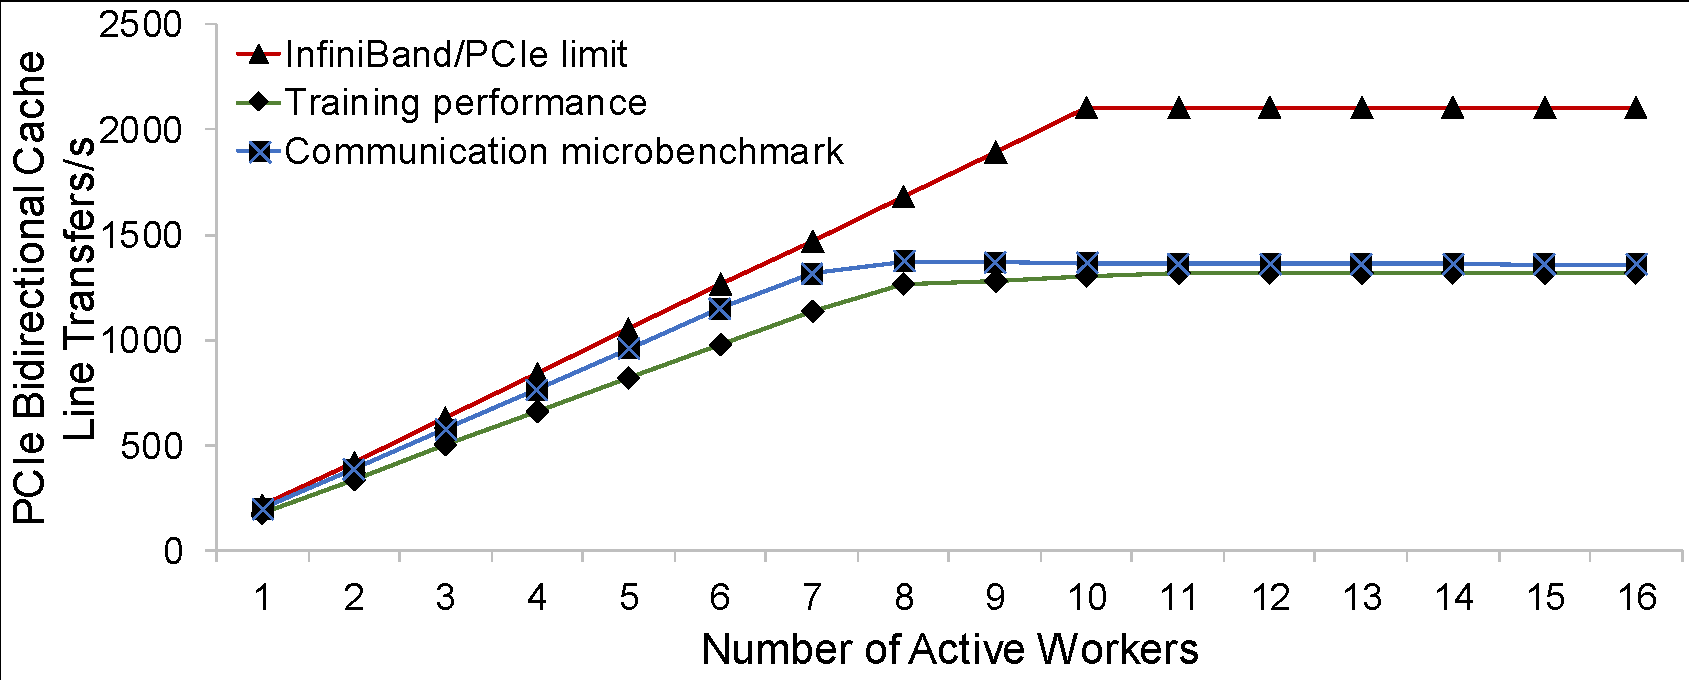
\includegraphics[width=.7\linewidth,trim=3 2 2 2,clip]{Figures/Scalability.pdf}
	\caption{\pbox{} scalability is limited by the throughput of the PCIe to the on-chip network bridge of the PBox processors. \phub{} can utilize 97\% of the measured peak PCIe bandwidth.}
	\label{fig:scalablity}
\end{figure}

Figure \ref{fig:scalablity} summarizes this experiment. The InfiniBand/PCIe limit line shows an ideal case where unlimited cache line transfers can be performed. However, this rate was not achievable even with a microbenchmark, which poses a hard upper bound on how fast \phub can run during training. We also see that, when training VGG with \code{ZeroComputeEngine}, as more workers are added, \pbox{}'s performance approached the microbenchmarks (97\%), demonstrating \phub{}'s ability to fully utilize system resources. The gap in the plot between \pbox and the microbenchmark %before they overlap 
is due to the overhead of scheduling operations in MxNet and straggler effects in workers. \pbox{} hit the limit at a sustained 80GB/s memory bandwidth.

In real training, however, \pbox{}'s scalability limit was difficult to reach. Recent work (\cite{keskar2016large, lecun1524efficient}) describes the difficulty of generalization with large batch sizes; it is not advantageous to blindly scale deep learning to a large number of workers without considering statistical efficiency~\cite{youspeeding, koliousiscrossbow}. One example \cite{ImageNetIn1Hour} reports that ResNet 50's statistical efficiency drops with aggregate batch sizes larger than 8192 on a system with 256 GPUs on 32 machines (with a mini-batch size of 32 per GPU). To assess whether \pbox could reach this scale, we measured the memory bandwidth usage for ResNet 50 with 8 workers using the same batch size. We found that \pbox required only 6GB/s memory bandwidth and an aggregated 4GB/s network bandwidth. This suggests that our \pbox prototype could scale to rack-level and support up to 120 worker machines training this network. In other words, our prototype could support sufficient scalability to handle cutting-edge training tasks.

On the other hand, the scalability bottleneck (PCIe controller) in our current prototype is specific to this particular platform, but it can change. For example, recently released AMD Epyc~\cite{AMDEpyc} processors provide nearly triple the Stream Triad performance
(290 GB/s)~\cite{EpycBenchmark} and 40\% more PCIe bandwidth than our
\pbox machine. We would expect Epyc to support 40\% more
throughput.
%Our test cluster does not have enough machines to saturate either of these, but we can project when scalability will stop based on these limits.


\subsection{Effectiveness of \pbox as a Rack-Scale Service}
\label{sec:hierarchicalEval}
We now evaluate effectiveness of \pbox as a rack-scale service with two typical scenarios in a 10 Gbps cloud-like environment: (1) when multiple jobs are training in parallel in a rack, sharing the same \pbox instance with different key namespaces and (2) when a training job crosses rack boundaries, and \phub performs hierarchical reduction.

\begin{figure}[t!]
    \centering
	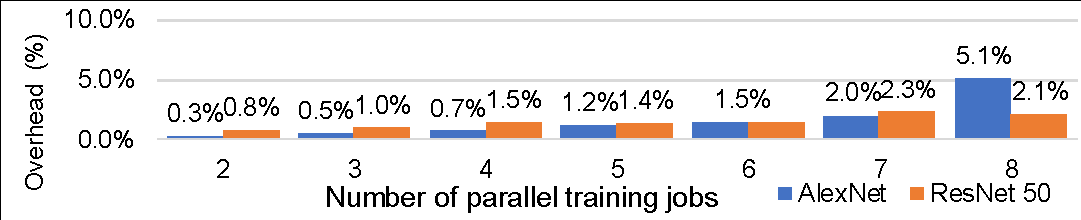
\includegraphics[width=.7\linewidth,trim=2 2 2 2,clip]{Figures/MultijobSim.pdf}
	\caption{Overhead of multiple parallel training jobs sharing the same \pbox instance.}
	\label{fig:multijobs}
\end{figure}

Figure \ref{fig:multijobs} shows the overhead of running multiple independent training jobs sharing a single \pbox. AlexNet saw a 5\% drop in per-job throughput when running 8 jobs, likely due to frequent invocation of optimizer and less effective caching; ResNet 50 saw a smaller impact as it is compute bound.

\begin{figure}[t!]
    \centering
	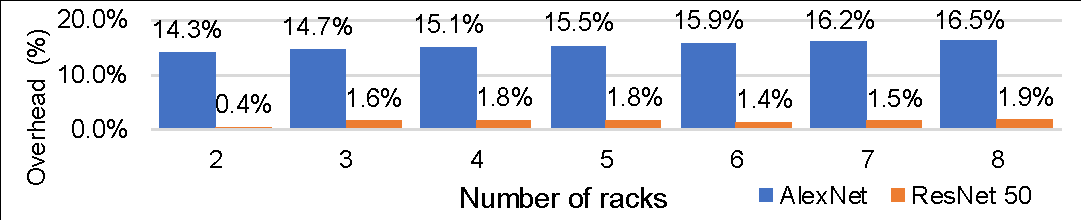
\includegraphics[width=.7\linewidth,trim=2 6 2 2,clip]{Figures/HierarchicalSim.pdf}
	\caption{Emulated overhead of hierarchical reduction with \pbox.}
	\label{fig:hierarchical}
\end{figure}

Figure \ref{fig:hierarchical} emulates a single cloud-based training job whose VMs span N racks, and each rack contains 8 workers and 1 \pbox. The \pbox uses a widely used ring reduction algorithm~\cite{baidures3:online,DBLP:journals/corr/abs-1802-05799} for inter-rack aggregation. 

Since we have only one \pbox machine, we model this ring reduction by sending and receiving N chunk-size messages sequentially, each performing one additional aggregation, for each of the keys, after local rack has finished aggregation. We assume each rack would finish its local aggregation at roughly the same time, as stragglers can exist regardless of rack assignment. Therefore, this faithfully estimates overhead of \phub{}'s hierarchical reduction.

AlexNet's throughput loss comes from added latency of multiple rounds of communication, but is compensated by drastically reduced cross-rack traffic, and thus we would expect speedup in real deployment. On the other hand, we again observed virtually no loss of throughput in ResNet 50.

\subsection{Rack-scale cost model}

Is a cluster built with PHubs and a slow network more cost effective than one with sharded PSs and a fast network? This section explores this question using a simple cost model. We consider the cost of three cluster components: worker nodes, PHub nodes, and network gear. We use advertised prices from the Internet; while a datacenter operator might pay less, the ratios between component prices should still be similar. The baseline is a cluster running MXNet IB with colocated sharded PSs; we compare this to a PHub deployment in terms of throughput per dollar.

The model works by computing the cost of a worker node, and adding to it the amortized cost of its network usage; for the PHub deployment, it also includes the amortized cost of the worker's PHub usage. This allows us to compare the cost of worker nodes in deployments with different numbers of workers per rack, switch, or PHub. We capture only the most significant cost, and include only capital cost, since operational costs are dominated by GPU power usage and thus differences would be small.

We model a standard three-layer datacenter network with some simplifying assumptions: racks hold as many machines as may be connected to a single switch, all switches and cables are identical, and oversubscription happens only at ToR switches. We model network costs by charging each worker the NIC per-port cost $N$, the amortized cost of one ToR switch port $S$ and cable $C$, and fractional costs of ToR/aggregation/core switch ports and cables depending on the oversubscription factor $F$. Thus, the amortized cost of the network per machine is $A=(N+S+C)+F(4S+2C)$. Since our goal is to model costs for future deployments, we make two changes from our experimental setup. Instead of 10Gb IB, we use 25 Gb Ethernet. Instead of NVIDIA 1080 Ti's, we assume a future GPU with similar cost $G$, but that performs like today's V100. This keeps the compute/communication ratio similar to that of our experiments. We use ResNet-50 for comparison; we use our 10Gb IB results for the PHub setting and downclocked 40Gb IB for the MXNet IB baseline. We include 2\% overhead in the PHub numbers to account for aggregation between racks.

%We use similar worker and PHub nodes as in our experiments. The cost $W$ is 

%% For the baseline, we use the same SuperMicro 1028GQ-TR worker nodes as in our evaluation, but with 4 GPUs. The advertised cost $W$ is \$4117~\cite{worker-price} without GPUs; we use the price of the NVIDIA GeForce 1080 Ti (\$699~\cite{nvidia-1080ti}) for the GPU price $G$. We use the Mellanox ConnectX-4 EN for 100Gb Ethernet (\$795~\cite{mellanox-eth}); the cost of a 2 meter cable is \$94~\cite{mellanox-cable}. The PHub worker nodes have the same configuration but with Mellanox ConnectX-4 Lx EN cards for 25Gb Ethernet (\$260~\cite{mellanox-eth}); the cable cost is \$31.25 using 4-to-1 breakout cables~\cite{mellanox-cable}. The PHub node is the same SuperMicro 6038R-TXR as in the evaluation; its cost $H$ is \$8407~\cite{phub-price}, and it uses 10 dual-port 25Gb Mellanox ConnectX-4 Lx EN cards (\$325~\cite{mellanox-eth}, or \$162.5 per port). We use the Arista 7060CX-32S 32-port 100Gb Ethernet switch (\$21077~\cite{}) in both configurations, with breakout cables to connect the 25Gb hosts. This means that with no oversubscription, a single switch can support 16 100Gb baseline workers, or a PHub and 44 25Gb workers. We assume 1 PHub per switch to allow for oversubscription; with 2:1 oversubscription each switch could support 65 25Gb workers; with 3:1 oversubscription, 76. The cost of each baseline worker is $W+N+4G+A$, and the cost of a PHub worker is $W+N+4G+A+KP$, where $KP$ is the amortized cost of the PHub ($P=W+20N$ and $K$ is the worker-to-phub ratio).

Workers are the same as in our evaluation, but with 4 GPUs. The cost $W$ is \$4117~\cite{worker-price} without GPUs; the GPU price $G$ is (\$699~\cite{nvidia-1080ti}). The 100Gb baseline uses Mellanox ConnectX-4 EN cards (\$795~\cite{mellanox-eth}) and 2m cables (\$94~\cite{mellanox-cable}). The 25Gb PHub workers use Mellanox ConnectX-4 Lx EN cards (\$260~\cite{mellanox-eth}) and 4-to-1 breakout cables (\$31.25 per port~\cite{mellanox-cable}).
The PHub node (also same as evaluation) cost $H$ is \$8407~\cite{phub-price}, plus 10 dual-port 25Gb Mellanox ConnectX-4 Lx EN cards (\$162.5 per port~\cite{mellanox-eth}). The cost of each baseline worker is $W+N+4G+A$, and the cost of a PHub worker is $W+N+4G+A+KP$, where $KP$ is the amortized PHub cost ($P=W+20N+20A$; $K$ is the worker to \phub ratio).

We use the Arista 7060CX-32S 32-port 100Gb Ethernet switch (\$21077~\cite{arista-price}) in both configurations, with breakout cables to connect 25Gb hosts.
With no oversubscription, each switch supports 16 100Gb baseline workers, or a PHub and 44 25Gb workers. With 2:1 oversubscription each switch could support a \phub and 65 25Gb workers; with 3:1, the number of supported workers is 76. 




%% \begin{table}[tb!]
%%   \centering
%%   \small
%%   \begin{tabular}{|r|c|c|c|}
%%     \hline
%%                   & Baseline         & PHub worker                & PHub \\
%%     \hline
%%     $W$ & \$4117~\cite{worker-price} & \$4117~\cite{worker-price} & \$8407~\cite{phub-price} \\
%%     $G$ & \$699~\cite{nvidia-1080ti} & \$699                      & \\
%%     $N$ & \$795~\cite{mellanox-eth}  & \$260                      & \$162.5/port \\
%%     $S$ & \$795~\cite{mellanox-eth}  & \$260                      & \$162.5/port \\
%%     \hline
%%   \end{tabular}
%%   \caption{Cost model parameters}
%%   \label{table:costModelParam}
%% \end{table}

\begin{table}[tb!]
  \centering
  \begin{tabular}{|r|c|c|c|}
    \hline
    & \multicolumn{3}{c|}{Throughput/\$1000} \\
    
                                 & Future GPUs & Spendy & Cheap \\
    \hline
    100Gb Sharded 1:1 &             46.11 &          14.57 &      60.41\\
    \hline 
    25Gb PHub     1:1 &             55.19 &          15.30 &      77.21\\
    \hline 
    25Gb PHub     2:1 &             57.71 &          15.49 &      82.24\\
    \hline 
    25Gb PHub     3:1 &             59.03 &          15.58 &      84.95\\
    \hline
  \end{tabular}
  \caption{Datacenter cost model comparing 25GbE PHub deployments with 100GbE MXNet IB on ResNet-50. Higher is better. The Future GPU PHub deployment with 2:1 oversubscription provides 25\% better throughput per dollar.}
  \label{table:costModel}
\end{table}

%% Table~\ref{table:costModel} compares a full-bisection-bandwidth 100GbE sharded MXNet IB deployment with 25GbE PHub deployments with varying oversubscription. With 2:1 oversubscription, the PHub deployment provides 26\% better throughput per dollar. We consider two other configurations. First, one using today's expensive V100s, where the 2:1 PHub deployment provides only 6\% better throughput per dollar: future GPUs this expensive are likely to be faster than this, so this configuration essentially provides a lower bound to improvement. Second, one using cheap (E5-2603 v4) in workers, providing 38\% better throughput per dollar: since the majority of training is done on the GPUs, CPU performance may not be important.

Table~\ref{table:costModel} compares a full-bisection-bandwidth 100GbE sharded MXNet IB deployment with 25GbE PHub deployments with varying oversubscription. With 2:1 oversubscription, the PHub deployment provides 26\% better throughput per dollar. We consider two other configurations: a ``lower bound'' using today's expensive V100's, where the 2:1 PHub deployment provides only 6\% improvement; and a ``GPU-focused'' one using cheap CPUs (E5-2603 v4) in workers, providing 36\% improvement.






\section{Effectiveness of \plink}
We continue to evaluate \plink in public cloud environments. 

Our evaluation goals are as follows: (1) Measure \plink{}'s impact on end-to-end training.  (2) Demonstrate the efficiency of \ha. (3) Quantify the benefit of hierarchical aggregation and topology-awareness. (4) Evaluate the accuracy of \marcopolo{}'s inference of physical affinity. (5) Assess how well \autoplink reacts to network changes. 

\subsection{Environment Setup}
\label{sec:commBackend}
We perform our experiments on both \azure and \ectwo, in the same region or availability zone. Each VM runs Linux kernel 4.18 with SoftiWarp support~\cite{zrliosof32:online}, Cuda 9.2, CuDNN 7, and network enhancements~\cite{Createan37:online, Enablean80:online} if possible. All VMs are provided with at least 10~Gbps network throughput, using DCTCP~\cite{data-center-tcp-dctcp} as SoftRoCE and SoftiWarp do not yield better performance. \ha uses a chunk size tuned to its best performance, usually 16 to 64KB. All experiments use 64 nodes unless otherwise specified. Some experiments involve comparing results generated with uncertainty. In those cases, we report speedup in terms of mean and percentile metrics together with performance distribution of 50 runs. Each sample represents mean performance of 20 iterations using a potentially different cluster assignment generated by the underlying mechanism. %, and each sample collected is the mean performance of 20 iterations. %We also interleave runs of different approaches to further reduce the interference from the environment, as suggested in~\cite{perfVariance}.

%To find the fastest transport layer for \ha, we use a benchmark that measures the median latency of 50 reduction runs of 512MB of data (sufficiently large for throughput measurement), on C5 and Standard D VMs on EC2 and Azure. We found our TCP implementation to be 1.07x and 5.94x faster than SoftiWarp and SoftRoCE implementations. We also found no significant performance differences among various TCP variants. In the following performance experiments, we use DCTCP~\cite{data-center-tcp-dctcp} as it keeps queueing delays low within a datacenter. To ensure our baselines get the best performance, we enforce all VMs to be in the same availability zone on EC2 and the same datacenter on Azure. \textsection\ref{sec:related} discusses the potential of \plink to accelerate cross-datacenter, cross-region training. In accuracy measurements, we allow VMs to span more hierarchy for a wider coverage.

%Some experiments report aggregation-only performance, and the setup will be specified individually. Some report end to end training performance of training popular neural network models in terms of throughput speedup. We omit accuracy result, as \plink optimizations do not change this. We found no big difference in throughput when training with Pytorch/Caffe2 or MxNet. Thus we report only Pytorch/Caffe2 performance. 
%We fit 8 samples/GPU. We did not use large batch optimizations in order to stress the communication part of the training pipeline without oversaturating the GPUs. See \ref{sec:related} for a discussion.

\begin{figure}[t!]
	\centering
	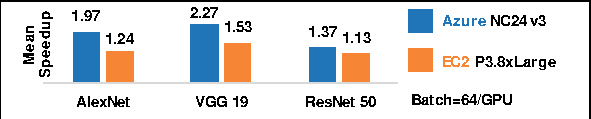
\includegraphics[width=.7\linewidth, trim=2 1 1 3,clip]{Figures/end2end.pdf}
	\caption{\plink{}'s collective optimizations achieve up to 2.27x speedup on  public clouds training popular neural network models, compared to original Pytorch/Caffe2.}
	\label{fig:end2end}
\end{figure}


\subsection{End to end training performance}
We start our evaluation with the impact of \plink{}'s collective optimizations on the end-to-end training performance of popular neural networks. Then we breakdown the effect of each optimization in the following sections. We compare \plink{} to original Pytorch/Caffe2 performance by replacing Gloo. We represent training speedup as mean speedup in throughput of 50 iterations to save experimental cost. This directly translates to a reduction in end-to-end training time as \plink{}'s optimization does not change convergence because it keeps the computation intact. %We use a batch size of 64/GPU on 64 P3.8xLarge nodes on \ectwo and Standard NC24v3 nodes on \azure, each with a V100 GPU. We simply generate 8 clusters with balance elasticity set to 2.

Figure~\ref{fig:end2end} shows the speedup of \plink, which ranges from 1.37-2.27x on \azure, and 1.13x-1.53x on \ectwo\footnote{While we report only data-parallel results for its dominance in distributed training, \plink optimizations are paradigm-agnostic, as all the scheduling of transfers is done by the framework.} when training popular vision models. We expect larger speedups for neural networks with higher communication to computation ratios (such as AlexNet and VGG) on VMs with faster networks, as we observe near line-rate network utilization when training them with \plink. For models with smaller communication to computation ratios (such as ResNet-50), \plink{}'s speedup comes from its reduced reduction latency.

\subsection{Efficiency of \ha}
\label{sec:baseline}
This section evaluates the performance of \ha itself, disabling \marcopolo{} and \autoplink{}. %. In particular we examine the performance gains achieved by \ha{} from efficient execution of aggregation schedules. % while \ref{sec:2lhaRandom} reveals the additional speedup from a \strongrandom-powered hierarchical scheme.
%\noindent\textbf{Comparison to other systems.}
For clarity, we first set up our baseline with communication libraries used in major training frameworks, including MxNet PS-Lite, Nvidia NCCL 2.4, and Facebook Gloo, covering ring (Gloo, NCCL), tree (NCCL), halving-doubling (Gloo) and parameter server (PS-Lite). %(\textsection\ref{sec:differentReductionAlgorithms}).
We use each library's benchmark program to measure its performance. On both \azure and \ectwo, we use instances with V100 GPUs and test end-to-end reduction performance
%~\cite{dmlcpsli50:online}
involving copying from/to a GPU. % The rest of experiment setup is same as in \textsection\ref{sec:commBackend}.

\begin{figure}[t!]
	\centering
	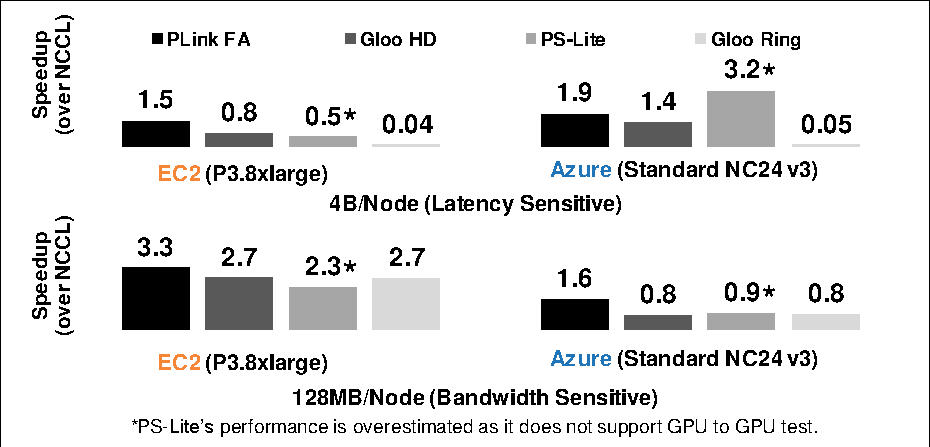
\includegraphics[width=.7\linewidth, trim=2 3 3 3,clip]{Figures/baseline.pdf}
	\caption{GPU to GPU aggregation speedup of various systems on \azure and \ectwo in terms of mean latency for large and small buffers, normalized to NCCL's performance. }
	\label{fig:baseline}
\end{figure}

\begin{figure}[t!]
	\centering
	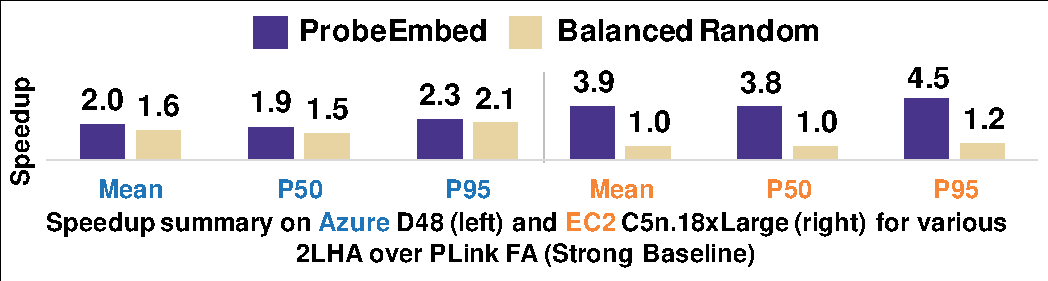
\includegraphics[width=.7\linewidth, trim=2 3 3 3,clip]{Figures/perfSummary.pdf}
	\caption{Mean, P50, and P95 additional speedup of \mlha using different approaches over FA (\strongbaseline). Run on 64 \azure D64 series and \ectwo C5n.18xLarge instances, with a constant VM topology throughout this experiment.}% See detailed analysis for each series in corresponding sections. ResNet-50 buffer sizes and distributions is used.}
	\label{fig:perfSummary}
\end{figure}

Figure \ref{fig:baseline} shows the speedup in terms of mean (20 iterations) GPU to GPU reduction latency normalized to NCCL's result of aggregating a large (128MB) and a small (4B) buffer. To provide a fair comparison, we limit \ha to use a single connection per peer (in a typical scenario, multiple connections are used). Overall, \ha{}'s flat aggregation (FA) leads the pack and is thus used as a \strongbaseline.

%\begin{table}
%        \centering
%        \footnotesize
%	\begin{tabular}{|c|c|c|c|c|c|c|}
%		\hline
%		Time (ms)   & 2 nodes & 4 & 8 & 16 & 32 & 64 \\
%		\hline
%		EC2  & 535   & 680   & 923  &  951 & 1270 & 1247  \\
%		\hline
%		Azure & 937 & 961 & 967 & 989 & 934 & 1031 \\
%		\hline
%	\end{tabular}
%	\caption{Reduction latency (512MB/node) vs number of nodes.}
%	\label{table:scalability}
%\end{table}

%\noindent\textbf{Scalability.}
%\label{sec:scalability} We also evaluated \ha{}'s scalability by varying the number of participating nodes on Azure, with a buffer size of 512MB. \ha achieves a 91\% scaling ratio from 2 to 64 nodes. This is because \ha{}'s chunking (\textsection\ref{sec:generatingAggregationPlan}) capability keeps per-node workload constant.

%The bumps of latency on EC2 as we add nodes is likely due to nodes are more spread as they are added in, as the latency of each iteration is determined by the bottleneck link in the full connection mesh. 
%so ideally, the reduction latency should not increase if each node can achieve full bandwidth goodput when communicating with rest of the nodes. Second, we notice the bumps of latency from 4 to 8 and 16 to 36 nodes on EC2, likely due to nodes are more spread as more are added in.

%\begin{table}
%        \centering
%        \footnotesize
%	\begin{tabular}{|c|c|c|c|}
%		\hline
%		Speedup   & \strongrandom  & Groundtruth & \marcopolo{}  \\
%		\hline
%		EC2  & 2.47   &  N/A   & 3.09   \\
%		\hline
%		Azure & 1.20 & 1.16 & 1.32\\
%		\hline
%	\end{tabular}
%	\caption{Aggregated relative speedup over FA (\strongbaseline) achieved on 64 Azure F16 series and EC2 C5n.18xlarge instances, with a constant VM topology throughout this experiment. See detailed analysis for each column in corresponding sections.}
%	\label{table:perfSummary}
%\end{table}

\subsection{Effectiveness of Hierarchical Aggregation}
\label{sec:2lhaRandom} 
We continue with a detailed comparison between \plink FA and \mlha, reducing a real-world model (ResNet-50, varying buffer sizes totalling~$\approx$100MB). We use 4 connections per peer to fully utilize VM bandwidth. We separately tuned chunk sizes to ensure baseline perform well in both clouds. We present the speedup summary in Figure~\ref{fig:perfSummary}; then, each subsection details the benefits associated with the individual technique. Performance distribution is found in Figure~\ref{fig:probeembedvsrandomvsflat}.  %Overall, \plink{} is able to achieve up to 4x mean and 4.5x P95 (95th percentile) speedup on \ectwo, and 2x mean and 2.3x P95 speedup on \azure compared to FA. 

%\subsubsection{\strongrandom-guided \mlha versus FA}
%\mlha can provide a performance benefit over FA without takig network locality into account by using \textit{\strongrandom}~(\textsection\ref{sec:marcopolo}) to generate schedules.  Figure \ref{fig:probeembedvsrandomvsflat} shows that, empirically, \strongrandom HA can achieve a mean speedup of 1.6x on \azure over FA, and is on par with FA's mean performance with shorter tail on \ectwo, whereas FA performance is highly volatile due to its sensitivity to network conditions as nodes communicate in an all-to-all pattern. %HA performance varies due to variability in the specific clusters generated for each run. Nonetheless, HA achieves both a lower expected reduction latency and a lower tail latency due to more localized communication.

%To improve our coverage, we ran the same experiments in additional configurations on Azure and EC2 (e.g., using the F, NC and E instances on Azure as well as G3 and P3 instances on EC2) and observed similar benefits. %Across all our experiments, on Azure, random \mlha performance beats FA by up to 1.7x; on EC2, the speedup is up to 3.9x. 
% Only in few cases do we fail to see a meaningful speedup of \mlha over FA.
%The speedup of random \mlha over FA comes from the traffic localization property of HA: only one copy of the buffer is transferred intercluster.
%While it is impractical to sample random performance across all physical configurations and clustering, we summarize our empirical finding on 64 Azure Standard F, Standard DS and Standard NC series VMs, as well as G3, C5 and P3 instances on EC2: 


\begin{figure}
	\centering
	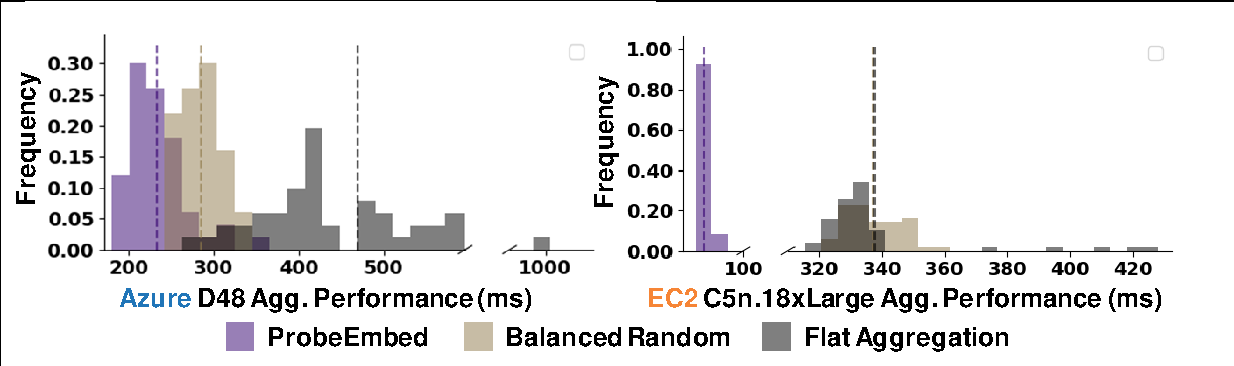
\includegraphics[width=.7\linewidth, trim=2 5 20 20,clip]{Figures/probeembedvsrandomvsflat.pdf}
	\caption{Empirical reduction latency distribution of \marcopolo-, \strongrandom- guided \mlha and FA on \azure and \ectwo.}
	\label{fig:probeembedvsrandomvsflat}
\end{figure}

%\subsubsection{\marcopolo{}'s Impact on \mlha Performance} This section highlights the benefit and necessity of \marcopolo{}, by comparing \marcopolo{}-guided \mlha with schedules crafted using ground-truth and \strongrandom.

\noindent\textbf{Comparing with ground-truth-guided \mlha.}
% \footnote{We did not obtain ground-truth information from EC2. However, we did experiments on EC2 that focused on inferring availability zone difference. Our high performance results in these experiments are unremarkable because cross availability zone communication has drastically higher latency.}, and focus our evaluation on Azure in this section.
Cloud providers can expose topology information to assist in locality-aware scheduling and communication. We obtain ground-truth topology information from \azure. We look at the effectiveness of using physical topology on \azure to form a reduction schedule for \mlha, grouping VM nodes based on their physical locality. % they are located in. %\arvind{are we saying that we don't group VMs inside a cluster for instance?  is the point that the cloud provider is providing only rack-level topo info?}


%We cluster nodes based on their physical residence (racks in this experiment). We used 64 Azure F instances for this experiment. In each run, the groundtruth-based clustering is fixed, while \marcopolo{} may generate different clusters. Thus we present speedup in terms of a measured performance distribution. The rest of the setup is kept the same as \ref{sec:2lhaRandom}.

%\begin{figure}
%	\centering
%	\includegraphics[width=\linewidth, trim=10 5 10 20,clip]{Figures/vsgroundtruth.pdf}
%	\caption{Empirical reduction performance distribution with \marcopolo{}-based clustering and groundtruth based clustering on two different spawns of 64 Azure F instances. \marcopolo{} leads groundtruth performance by 1.9x and 2x, and has lower performance variance.}
%	\label{fig:vsgroundtruth}
%\end{figure}

%We respawn the VMs multiple times to obtain different topologies in order to understand how they affect \mlha performance. For the runs shown in Figure~\ref{fig:perfSummary}, \marcopolo-guided \mlha beats ground-truth-guided \mlha by 7.1x for Azure (which is the setting where we were able to obtain ground-truth data). % and these 64 VMs are spread across 22 racks, with the largest rack containing 8 VM nodes while the smallest containing only 1. In two other occasions, these 64 VMs landed in 17 racks and 40 racks respectively, and \marcopolo{} achieves 1.9x and 2.0x speedup over ground-truth-guided approach.

Our experiment shows that \marcopolo-guided \mlha beats ground-truth-guided \mlha by 1.15x on average. The performance of ground-truth-guided \mlha relies on a ``luck'' factor related to the physical topology of the VM nodes: the more compactly the VMs are allocated, and the more balanced the allocation in each rack is, the better performance of ground-truth-guided \mlha should be. But VM spawn location is in total control of the scheduler, and sometimes it is impossible to guarantee a compact allocation due to current VM occupancy. It is difficult to splice/split undersized/oversized racks for a more balanced \mlha without probing for network properties, which \marcopolo{} does.


%\ref{fig:vsgroundtruth} illustrates this: a more compact allocation (64 VM nodes in 17 racks) does generate better performance and less variation than a more scattered allocation (64 VM nodes in 40 racks). But in both cases \marcopolo{}-guided \mlha beats groundtruth-guided \mlha by 1.9x and 2x respectively. Our further scrutiny shows the reason are (1) more compact allocation does not mean more balanced allocation, and without running network probes, it is difficult to splice or split undersized or oversized clusters to form a balanced \mlha plan, and (2) groundtruth-based approaches ignores completely the dynamic property of the network, which shifts how VM clusters are generated.

\noindent\textbf{Comparing with \strongrandom-guided \mlha.}
%marcopolo{}'s goals are to determine the number of clusters to generate, and returns clustered nodes. 
We observe an additional 1.3x and 3.9x expected performance gain of the clusters generated by \marcopolo{} over those of \strongrandom{} on \azure and \ectwo. \marcopolo{} leads to  better and more stable performance by generating cohesive, locality-preserving group assignments. On the other hand, \strongrandom can include VMs that are far away in the same group, creating a bottleneck in the system. %Our experience also indicates larger VM instances often have larger speedups with \marcopolo{}, perhaps because they are less likely to be packed into the same physical host, resulting in a low inherent locality. %, which is harder for \strongrandom to capture. %is likely to generate groups whose intra-group distance is similar to the diameter of the ring, by picking equally-spaced VM nodes on the circumference of the ring, which may result in lower variance but with less-than-ideal performance.

%One interesting observation is the three peaks in C5n's distribution. This may be due to the stochastic process of kmeans: for example, the lonely VM nodse on the upper-left can be partitioned into multiple clusters, resulting in different performance. Different initializations for the embedding process can also contribute to landing in different local minima in the optimization manifold.

%Across all experiments, we found \marcopolo{}-guided \mlha has a speedup range of 1.04x to 1.5x and 1.02 to 1.25x over random-guided \mlha on Azure and EC2, respectively. While \strongrandom can generate all possible clusters, \marcopolo{} effectively ''cherrypicks`` a smaller portion of the partitioning space that better preserves locality, leading to higher performance in expectation. Our experience also indicates larger VM instances often lead \marcopolo{} to have larger speedup gains, likely because they are less likely to be packed into the same physical host, causing VMs to spread across more physical hosts, resulting in less inherent locality, making it harder for \strongrandom to capture incidentally. % which \strongrandom is less likely to capture incidentally. %We also find larger instances usually lead to larger speedup, and this is likely due to the fact that smaller instances can be ''packed`` into a physical host, allowing more chance for \strongrandom to capture locality. In general, our observation indicates \marcopolo{}'s performance distribution has lower standard deviation compared to that of \strongrandom{}'s in general.


\begin{figure}
	\centering
	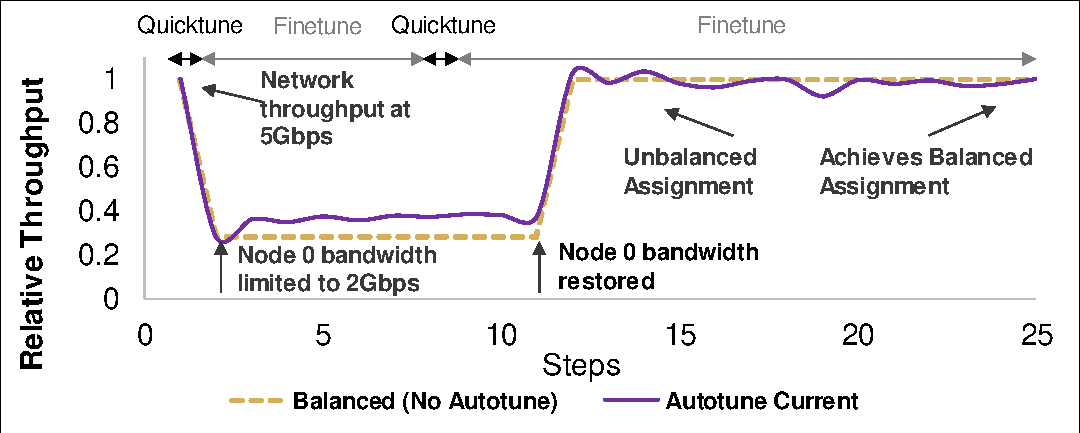
\includegraphics[width=.7\linewidth, trim=2 1 3 3,clip]{Figures/autotunebw.pdf}
	\caption{\autoplink adapts to bandwidth changes by assigning LMs based on current metrics of \ha. Dotted lines: averaged throughput. Solid lines: snapshot throughput.}
	\label{fig:autotunebw}
\end{figure}


%Surprisingly, we found \plink sustains a stable speedup of 1.5x on both Azure and EC2 with V100 GPUs, up to a batch size of 64 (at which point no more samples can be filled in). This suggests that with a fast modern GPU, memory becomes a bottleneck before computation, and thus \plink{}'s communication acceleration is valuable even with a large batch size. 



\subsection{Accuracy of \marcopolo{}}
\label{sec:accuracy}
Effective exploitation of locality requires capturing both static and dynamic aspects of the network (which is directly captured by the probes). %\marcopolo explicitly measures dynamic network properties and uses this information to infer static network topology. 
In this section, we evaluate \marcopolo{}'s ability to discover the network topology in terms of \textit{physical affinity}.
%from three angles: (1) the accuracy of different types of network probes; (2) the ability of \marcopolo{} to accurately infer VM physical affinity; and (3) the effectiveness of using embedding as a denoising technique.%(1) the accuracy of network probes used by \marcopolo{}; (2) the ability to accurately infer VM physical affinity and (3) the effectiveness of using embedding as a de-noising technique.

%\subsubsection{Physical Affinity Inference Accuracy (PAIA)}
\noindent\textbf{Physical Affinity Inference Accuracy (PAIA).}
We define \textit{affinity score} as an intuitive metric to quatify how well \marcopolo{} captures network topology: for any two VM nodes $(a,b)$ that have comparable distance to an observer $c$, let $T(a,c), T(b,c)$ be the ground-truth distance (in terms of hops) from $a$ to $c$ and $b$ to $c$, and let $M(a,c), M(b,c)$ be the \marcopolo{} measured distance. We define an affinity score $A(a,b,c)$ for triplet $(a,b,c)$ as:
%
\begin{align*}
\small
  A(a,b,c) = 
   \left\lbrace
  \begin{array}{l@{}l}
    1 \textbf{ if $M(a,c) < M(b,c)$ and $T(a,c) < T(b,c)$}\\
    \textbf{\quad or $M(a,c) > M(b,c)$ and $T(a,c) > T(b,c)$} \\
    0 \text{ otherwise}
  \end{array}
  \right.
\end{align*}

For a given $c$, $A(a,b,c)$ captures whether \marcopolo{}'s measurement agrees with the actual hop distance between $a$ and $b$. $A(a,b,c)$ is only defined for \textit{comparable} nodes $a$ and $b$ to $c$: each node's position is encoded as a tuple of format %\code{region:datacenter:cluster:row:rack:host}. 
(region, datacenter, cluster, row, rack, host).
$a$ and $b$ are comparable to $c$ if they have different longest common prefix to $c$. Longer common prefix means higher affinity. We now define PAIA as the total sum of all $A(a,b,c)$ over the count of all defined $A(a,b,c)$s. A higher PAIA means a better comprehension of the datacenter network.


%\subsubsection{Quality of Various \marcopolo{} Probes}
\noindent\textbf{Quality of Various \marcopolo{} Probes.}
We evaluate base affinity accuracy achieved by running latency and bandwidth probes, without the embedding process, on 64 VMs, in 2 datacenters, 7 clusters, 15 rows and 61 racks in the US West 2 region with a total of 81.3K triplets to infer. Latency-based measurements better reflect underlying topology, with the DPDK Echo probe yielding a PAIA score of 95.6\% compared to 77.4\% with iperf, likely because bandwidth is not necessarily determined by distance. % Particularly, %. %Thus, our performance evaluations are all DPDK Echo-based.

%To evaluate with different VM allocations and topologies, we repeat the process of VM reallocation and reprobe, with DPDK's base affinity score ranging from 0.39 to 1.0.

%In general, we find 

%We repeat the process of deallocation and reallocation of VM multiple times, and each time involves a reprobing process. We report the best accuracy score achieved by each probe\footnote{For probes that measure affinity, such as iperf and NTTTCP, we convert affinity to distance using $D = 1. / (P / max(P))$, where $D$ and $P$ are the distance and probing matrix.}.

%\begin{table}[!htb]
%	\begin{minipage}{.45\columnwidth}
%		\centering
%	    \scriptsize	
%		\begin{tabular}{|c|c|}
%			\hline
%			DPDK Echo & iperf \\
%			\hline
%			98.1\% & 61.8\% \\
%			\hline
%		\end{tabular}
%		\caption{PAIA of various probes for 89 VMs in 2 datacenters, 6 clusters, 7 rows and 43 racks on \azure. Total triplets: 215K. }
%		\label{table:rawaffinityscore1}
%	\end{minipage}\quad
%	\begin{minipage}{.45\columnwidth}
%		\centering
%	    \scriptsize	
%			\begin{tabular}{|c|c|}
%				\hline
%				DPDK Echo & iperf \\
%				\hline
%				98.1\% & 61.8\% \\
%				\hline
%			\end{tabular}
%			\caption{PAIA of various probes for 89 VMs in 2 datacenters, 6 clusters, 7 rows and 43 racks on \azure. Total triplets: 215K. }
%			\label{table:alphaembedding}
%	\end{minipage}
%\end{table}


% across the order of 50k affinity triplets. % In many cases, we even find DPDK echo scoring all $A(a,b,c)$ instances correct.

%\subsubsection{Embedding's Effect on Affinity Inference}
\noindent\textbf{Embedding's Effect on Affinity Inference.}
\marcopolo{}'s probe readings can be affected by measurement noise. We now show how the embedding boosts \marcopolo{}'s inference accuracy, in a case with 64 VMs in a single datacenter with 75.2K triplets. This effectively shrinks the latency distribution and makes it more difficult to infer topology. DPDK Echo probes without embedding yield a PAIA score of 81.3\%. We apply embeddings with different $\alpha$ values to this dataset and found an average PAIA improvement of 5.0\% with $\alpha=1$, and 8.1\%  with $\alpha=2$.%, a 10\% improvement over the result without embedding.

%shown in Table~\ref{table:rawaffinityscore}. We observe non-trivial boosts in accuracy across all probes, demonstrating \marcopolo{}'s denoising effects. Across our experiments, we found 1\%-23\% boost in accuracy when embedding is helpful. However, embedding is not a panacea, and it does not help when the base accuracy is too low or already high. % Our performance evaluation used DPDK Echo measurements for clustering for its high accuracy.% We also found that the correlation between bandwidth readings and network topology is weak. We verified this by observing that probes achieve full line-rate transfers across the datacenter in Azure, albeit at a higher latency. We omit their ``boosted'' results in the table. 



%\begin{table}
%        \centering
%        \footnotesize
%	\begin{tabular}{|c|c|c|c|}
%		\hline
%		 & 16 nodes & 32 nodes & 64 nodes      \\
%		\hline
%		Azure D       & 0.78 + 0.07 (970)  & 0.85 + 0.04 (12894) & 0.72 + 0.23 (50602)    \\
%		\hline
%		Azure F       & 0.97 + 0 (1050)  & 0.88 + 0.04 (7818)  & 0.80 + 0.14 (61808)    \\
%		\hline
%	\end{tabular}
%	\caption{Embedding (dimension 2) helps boost affinity inference accuracy in noisy environment. Cell format: base accuracy + boost accuracy (total number of defined affinity triplets).  }
%	\label{table:embeddingBoost}
%\end{table}

%We continue to work on Azure D and F nodes, and vary the number of nodes to have a better coverage of both large and small number observations of distance are present. The result is summarized in Table~\ref{table:embeddingBoost}. We observe significant boost of accuracy in  occasions where base accuracy is slightly less than ideal. However, embedding is not panacea. We also found embedding less helpful when the base accuracy is too low or very high. 



\subsection{Effectiveness of \autoplink}
We conclude our evaluation with the real-world impact of \autoplink on training ResNet-50 with Pytorch/Caffe2 on 8 nodes with FA. We report \autoplink's effects in terms of end-to-end training performance. We run \autoplink continuously, ignoring the stop condition, and assess how \autoplink adapts to bandwidth changes and discovers a balanced LM assignment. We start by imposing no limits on bandwidth; then we limit the bandwidth of node 0, and eventually restore it. This shows how instantaneous training throughput changes as we apply \autoplink decisions.

Figure \ref{fig:autotunebw} shows this process. We perform a step of \autoplink every 10 iterations and report the snapshot reading of current throughput after the schedule change. %\footnote{We ignore the small overhead of changing plan in this experiment as it drastically exaggerates the frequency of \autoplink operations.}. 
At step=0, node 0's network throughput is $\approx$5~Gbps. At step=1, we limit its bandwidth to 2~Gbps. This causes an immediate drop in training performance and triggers \autoplink at step=3. Quicktune moves LMs away from node 0. The training throughput then bumps up immediately, and \autoplink enters fine-tuning mode through step=11. During this period, \autoplink continues to move LM assignments away from 0. When 0 is out of LMs, Finetune moves LMs among the rest of the nodes based on their blame score. At step=11, node 0's bandwidth is restored, causing an immediate jump in training performance, but this time node 0 is underloaded. At step=12, this is partially corrected by Quicktune. \autoplink continues to monitor and rebalance workloads throughout, arriving at a balanced assignment at t=25, with $\frac{max_n\sum_{i}{D(n,i)}}{min_n\sum_{i}{D(n,i)}} < 1.05$. Compared to using this near optimally balanced LM assignment alone, \autoplink delivers 1.27x speedup when node 0 is the bottleneck, and can quickly recover when node 0's limit is lifted. 


%The detection sensitivity for loss of performance of \autoplink depends on how bandwidth demanding the neural network is. We found \autoplink benefits more for models with larger communication sizes, such as AlexNet or VGG.






% With each model, we vary the batch size of each GPU to understand how the communication to computation ratio affects \plink{}'s effectiveness. Figure~\ref{fig:end2end} shows the speedup of \plink, ranging from 1.45x-3.04x on Azure, and 1.04x-1.75x on EC2. Unsurprisingly, \plink shows much larger speedups on models with higher communication to computation ratios than ones with lower ratios. In particular, training ResNet-50 on 64 VM nodes requires no more than 7~Gbps bandwidth, and speedup for \plink in this case comes from its reduced reduction latency. We also observe, surprisingly, that \plink{}'s effect is not very sensitive to the batch size chosen. %, and thus can deliver (albeit smaller) speedup even when the GPU memory is entirely full. We believe the difference in terms of speedup from the clouds come partially from how GPU clusters is organized, and partially from the fact that the relative speedup of \ha over halving doubling also differs across clouds (Figure~\ref{fig:baseline}).



\section{Effectiveness of PLink Collectives}
We evaluate the effectiveness of \cmpi with a series of microbenchmarks from various communication backends and real-world applications that uses \collectives algorithms, in public clouds. We represent speedup by comparing the performance we get from the best rank ordering and worst rank ordering. We opt to avoid comparing with the original rank ordering because it is random, and has a wide performance distribution (Figure~\ref{fig:azringperformance}).

\subsection{Experimental Setup}
Our experiments are conducted on two public clouds, \azure and \ectwo. We enable network acceleration on both clouds, and set TCP congestion control protocol to DCTCP. We include microbenchmarks that exercise ring, having doubling, double binary tree and bcube algorithms.  All experiments run on Ubuntu 19 with kernel 5. We mainly focus our evaluation on one of the most important \collectives tasks, \textit{allreduce} for its popularity and generality. %We use unmodified Facebook Gloo~\cite{glooalgo70:online}, OSU MPI microbenchmark~\cite{10.1007/978-3-642-33518-1_16} and Nvidia NCCL~\cite{NVIDIACo76:online} with OpenMPI 4. We use lightgbm~\cite{Ke2017LightGBMAH} to evaluate the real-world impact of \cmpi. 

\subsection{Prediction Accuracy of Cost Model}
While the goal of the cost model is not to predict the actual performance, but rather, it should preserve the relative order of performance, i.e., $p_{pred}(\mathbb{R}_1) < p_{pred}(\mathbb{R}_2) \implies p_{real}(\mathbb{R}_1) < p_{real}(\mathbb{R}_2)$ should hold true for as many pairs of $(R_i, R_j)$s as possible. Because our optimization goal is a lower cost value. We demonstrate this for ring based \mpi algorithms by generating 10 different rank orders, with the $i$-th order approximately corresponds to the $10i$-th percentile in the range of costs found by the solver. We obtain performance data for Facebook Gloo and OpenMPI running OSU Benchmark on 64 F16 nodes on \azure and 64 C5 nodes on \ectwo. We then compute Spearman~\cite{spearman} correlation coefficient between the predicted performance and the actual performance for each setup~(Table~\ref{table:correlation}). 

\begin{table}[t!]
	\centering
	\footnotesize
	\begin{tabular}{|c|c|c|}
		\hline 
	    Setup & Azure & EC2  \\
		\hline
		Gloo Ring 100MB      & 0.58 & 0.78  \\
		\hline
		OpenMPI Ring 100MB      & 0.81 & 0.94 \\
		\hline
	\end{tabular}
	\caption{Spearman correlation coefficient between predicted performance from cost model and actual performance.}
	\label{table:correlation}
\end{table}

%Figure~\ref{fig:azringperformance} shows where the predicted best (purple dotted line) and worst performance (black dotted line) using the cost model landed in the performance distribution from 500 random ordering: the $\mathbb{R}$ that is predicted to achieve worst/best performance falls in the 99th/1st percentile of the total observed distribution. While not perfect, we believe this is acceptable due to the imperfection of the cost model and limitation of solvers. 

\subsection{Microbenchmark Performance}
We now evaluate \cmpi{}'s efficacy with microbenchmarks of \mpi algorithms introduced earlier. We report mean speedup of 20 iterations. We run all benchmarks with 512 F16 nodes on \azure, except for NCCL, which runs on 64 P3.8xLarge GPU nodes on \ectwo. Particularly, we set $B=4$ for BCube; for NCCL, we use a single binary tree reduction for small buffers, and ring for large buffers. In all benchmarks we reduce a buffer of 100MB, except for Nvidia NCCL, where we reduce a small buffer of 4B to trigger the tree algorithm.


\begin{figure}[t!]
	\centering
	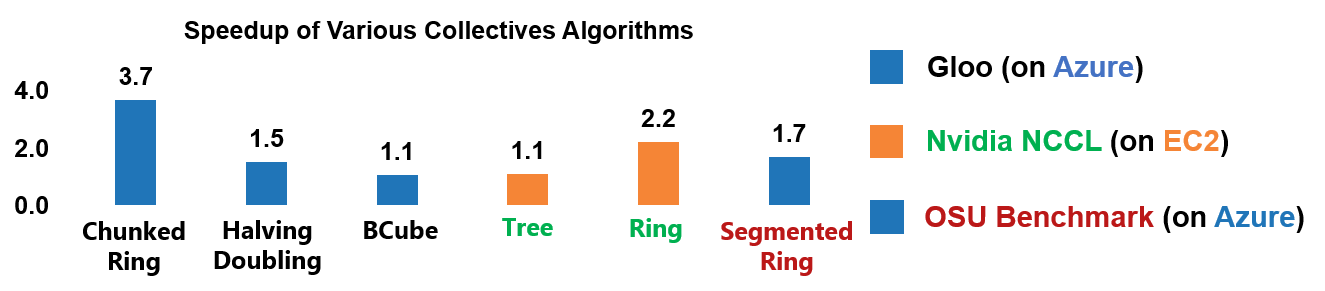
\includegraphics[width=.6\linewidth]{Figures/collectivesperformance.png}
	\caption{Speedups achieved by just using the rank ordering produced by our tool in various \collectives algorithms across multiple distributed communication backends at a large scale.}
	\label{fig:collectivesPerformance}
\end{figure}

Figure~\ref{fig:collectivesPerformance} shows a summary of speedups achieved using \cmpi on these benchmarks, ranging from 1.1x-3.7x, with the ring-family algorithms benefiting the most. We speculate the reason for the effectiveness is that they have a much wider performance distribution, as each permutation of the order can potentially generate a different performance (cost of each hop is on the critical path); they also have simpler cost model, allowing the solvers to quickly navigate the objective landscape. On the other hand, halving doubling, BCube and tree algorithms have complex objectives -- sum of maximums, resulting in a narrower performance distribution because mutation of the ordering may not change the cost at all if the mutation does not cause critical path to change. %This adds to difficulty of minimizing the objectives, because the solver itself relies on efficiently generating new cost values to proceed. 

\subsection{End-to-end Performance Impact on Real-world Applications}
\noindent \textbf{Speedup Distributed Gradient Boosted Decision Tree Training}. We evaluate \cmpi{}'s impact on LightGBM~\cite{Ke2017LightGBMAH}, a gradient boosted decision tree training system. We use data parallelism to run \textit{lambdarank} with metric \textit{ndcg}. Communication-wise, this workload runs two \collectives tasks: \textit{allreduce} and \textit{reducescatter}. %Each call to \textit{allreduce} reduces 24B of data, and approximately 1KB for \textit{reducescatter}. 
These two tasks are called sequentially when considering all tree leaves for split in each iteration, resulting in very frequent invocations. At our scale of 512 nodes, LightGBM automatically chooses to use halving and doubling for both \textit{reducescatter} and \textit{allreduce}. We use a typical dataset that represents an actual workload in our organization with 5K columns and a total size of 10GB for each node. We train 1000 trees, each with 120 leaves. We exclude the time it takes to load data from disk to memory, and report average speedup of 1000 iterations. \cmpi generated rank ordering speeds up training by 1.3x.

\noindent \textbf{Speedup Distributed Deep Neural Network Training}. We show \cmpi{}'s effectiveness on distributed training of DNNs with Caffe2/Pytorch, on 64 EC2 p3.8xLarge nodes with data parallelism and batch size of 64/GPU. We train AlexNet on ImageNet dataset. Since our \cmpi{} does not change computation and only improves communication efficiency of the \textit{allreduce} operation at iteration boundary, we report speedup of training in terms of images/second, averaged across 50 iterations. We use the ring chunked algorithm which achieves the best baseline performance, and the \cmpi{}-optimized rank ordering of VM nodes achieves a speedup of 1.2x.


\chapter{Conclusion}
The surge of data volume and accelerator throughput demand new optimizations in communication to accelerate distributed learning. This paper argues deficiency in communication comes from hardware, software and the network infrastructure itself. Through co-designing of software and hardware and careful probing and exploiting of locality in the physical network, we demonstrate significant end-to-end training speedup can be obtained.

\bibliographystyle{plain}
\bibliography{uwthesis}

\end{document}
